\documentclass[12pt]{extarticle}
\usepackage[paperwidth=15in,paperheight=7.2in]{geometry}
\usepackage{amsmath}
\usepackage{hyperref}
\usepackage{multirow}
\usepackage{pdfpages}
\usepackage[utf8]{inputenc}
\title{Kaon mixing: chiral and continuum extrapolations}
\author{R Mukherjee}
\date{\today}
\begin{document}
\maketitle
\tableofcontents
\clearpage
\section{$B_1$}
\begin{table}[h!]
\begin{center}
\begin{tabular}{|c|c|c|c|c|c|}
\hline
$\mu$ (GeV) & $a^2$, $m_\pi^2$& $a^2$, $m_\pi^2$ (no C)& $a^2$, $a^4$, $m_\pi^2$& $a^2$, $m_\pi^2$, $m_\pi^4$& $a^2$, $m_\pi^2$, $\log(m_\pi^2/\Lambda^2)$\\
\hline
2.4& \hyperlink{VVpAA/a2m2_24.pdf.1}{\textbf{0.5213(10)}: 2.342 (0.039)} & \hyperlink{VVpAA/a2m2noC_24.pdf.1}{\textbf{0.5271(46)}: 1.22 (0.295)} & \hyperlink{VVpAA/a2a4m2_24.pdf.1}{\textbf{0.5294(79)}: 2.664 (0.031)} & \hyperlink{VVpAA/a2m2m4_24.pdf.1}{\textbf{0.5233(12)}: 0.993 (0.41)} & \hyperlink{VVpAA/a2m2logm2_24.pdf.1}{\textbf{0.51075(99)}: 9.014 (0.0)}\\
2.0& \hyperlink{VVpAA/a2m2_20.pdf.1}{\textbf{0.5264(11)}: 1.838 (0.102)} & \hyperlink{VVpAA/a2m2noC_20.pdf.1}{\textbf{0.5310(48)}: 0.864 (0.421)} & \hyperlink{VVpAA/a2a4m2_20.pdf.1}{\textbf{0.5326(82)}: 2.159 (0.071)} & \hyperlink{VVpAA/a2m2m4_20.pdf.1}{\textbf{0.5282(12)}: 0.639 (0.635)} & \hyperlink{VVpAA/a2m2logm2_20.pdf.1}{\textbf{0.5157(10)}: 8.193 (0.0)}\\
1.8& \hyperlink{VVpAA/a2m2_18.pdf.1}{\textbf{0.5293(14)}: 1.315 (0.254)} & \hyperlink{VVpAA/a2m2noC_18.pdf.1}{\textbf{0.5328(53)}: 0.478 (0.62)} & \hyperlink{VVpAA/a2a4m2_18.pdf.1}{\textbf{0.5335(91)}: 1.6 (0.171)} & \hyperlink{VVpAA/a2m2m4_18.pdf.1}{\textbf{0.5310(14)}: 0.307 (0.873)} & \hyperlink{VVpAA/a2m2logm2_18.pdf.1}{\textbf{0.5188(13)}: 6.778 (0.0)}\\
1.5& \hyperlink{VVpAA/a2m2_15.pdf.1}{\textbf{0.5338(19)}: 0.734 (0.598)} & \hyperlink{VVpAA/a2m2noC_15.pdf.1}{\textbf{0.5356(64)}: 0.159 (0.853)} & \hyperlink{VVpAA/a2a4m2_15.pdf.1}{\textbf{0.536(11)}: 0.909 (0.457)} & \hyperlink{VVpAA/a2m2m4_15.pdf.1}{\textbf{0.5352(18)}: 0.099 (0.983)} & \hyperlink{VVpAA/a2m2logm2_15.pdf.1}{\textbf{0.5237(19)}: 4.464 (0.0)}\\
\hline
\end{tabular}
\caption{Physical point value from chiral and continuum extrapolation at renormalisation scale $\mu$. Entries are \textbf{value(error)}: $\chi^2/\text{DOF}$ ($p$-value).}
\end{center}
\end{table}
\begin{table}[h!]
\begin{center}
\begin{tabular}{|c c|c|c|c|c|c|}
\hline
$\mu$ (GeV) &  & $a^2$, $m_\pi^2$& $a^2$, $m_\pi^2$ (no C)& $a^2$, $a^4$, $m_\pi^2$& $a^2$, $m_\pi^2$, $m_\pi^4$& $a^2$, $m_\pi^2$, $\log(m_\pi^2/\Lambda^2)$\\
\hline
\multirow{2}{0.5in}{2.4} & $\alpha$ & 0.1001(70)& 0.040(52)& -0.043& 0.0864(83)& 0.1218(71)\\
 & $\beta$ & 0.00264(14)& 0.00221(27)& 0.00268(15)& 0.00016(89)& -0.0019(15)\\
\hline
\multirow{2}{0.5in}{2.0} & $\alpha$ & 0.0939(73)& 0.047(53)& -0.015& 0.0813(84)& 0.1150(74)\\
 & $\beta$ & 0.00262(14)& 0.00223(28)& 0.00265(15)& 0.00030(90)& -0.0020(15)\\
\hline
\multirow{2}{0.5in}{1.8} & $\alpha$ & 0.0894(84)& 0.055(57)& 0.016& 0.0781(89)& 0.1088(85)\\
 & $\beta$ & 0.00262(15)& 0.00225(29)& 0.00264(15)& 0.00039(94)& -0.0020(15)\\
\hline
\multirow{2}{0.5in}{1.5} & $\alpha$ & 0.081(10)& 0.066(65)& 0.036& 0.0722(99)& 0.098(10)\\
 & $\beta$ & 0.00261(15)& 0.00230(34)& 0.00261(16)& 0.001& -0.0020(15)\\
\hline
\end{tabular}
\caption{Fit values of coefficients in $B = B_0(1 + \mathbf{\alpha} a^2 + \mathbf{\beta} \frac{m_\pi^2}{f_\pi^2} + \ldots)$.}
\end{center}
\end{table}
\begin{figure}
\centering
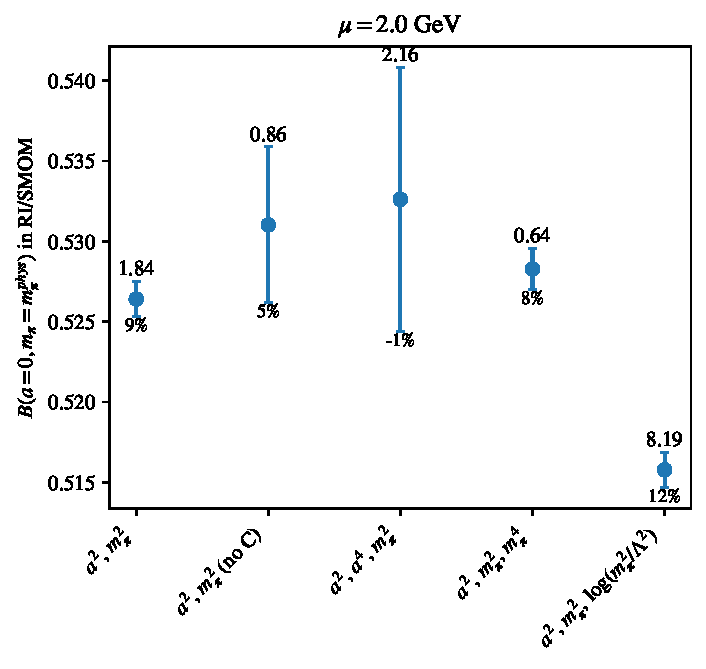
\includegraphics[page=1, width=1.1\textwidth]{plots/VVpAA_fit_summary.pdf}
\caption{\\(left) $B_{phys}$ in RI/SMOM scheme from fit variations (fits with $p$-value $<0.05$ marked with ``$\times$"). \\(right) $B_{phys}$ in $\overline{MS}$ computed using $B^{\overline{MS}} = R^{\overline{MS}\leftarrow SMOM}(3.0)\sigma_{npt}^{F1M}(3.0, 2.0) B^{SMOM}$.}
\end{figure}
\clearpage
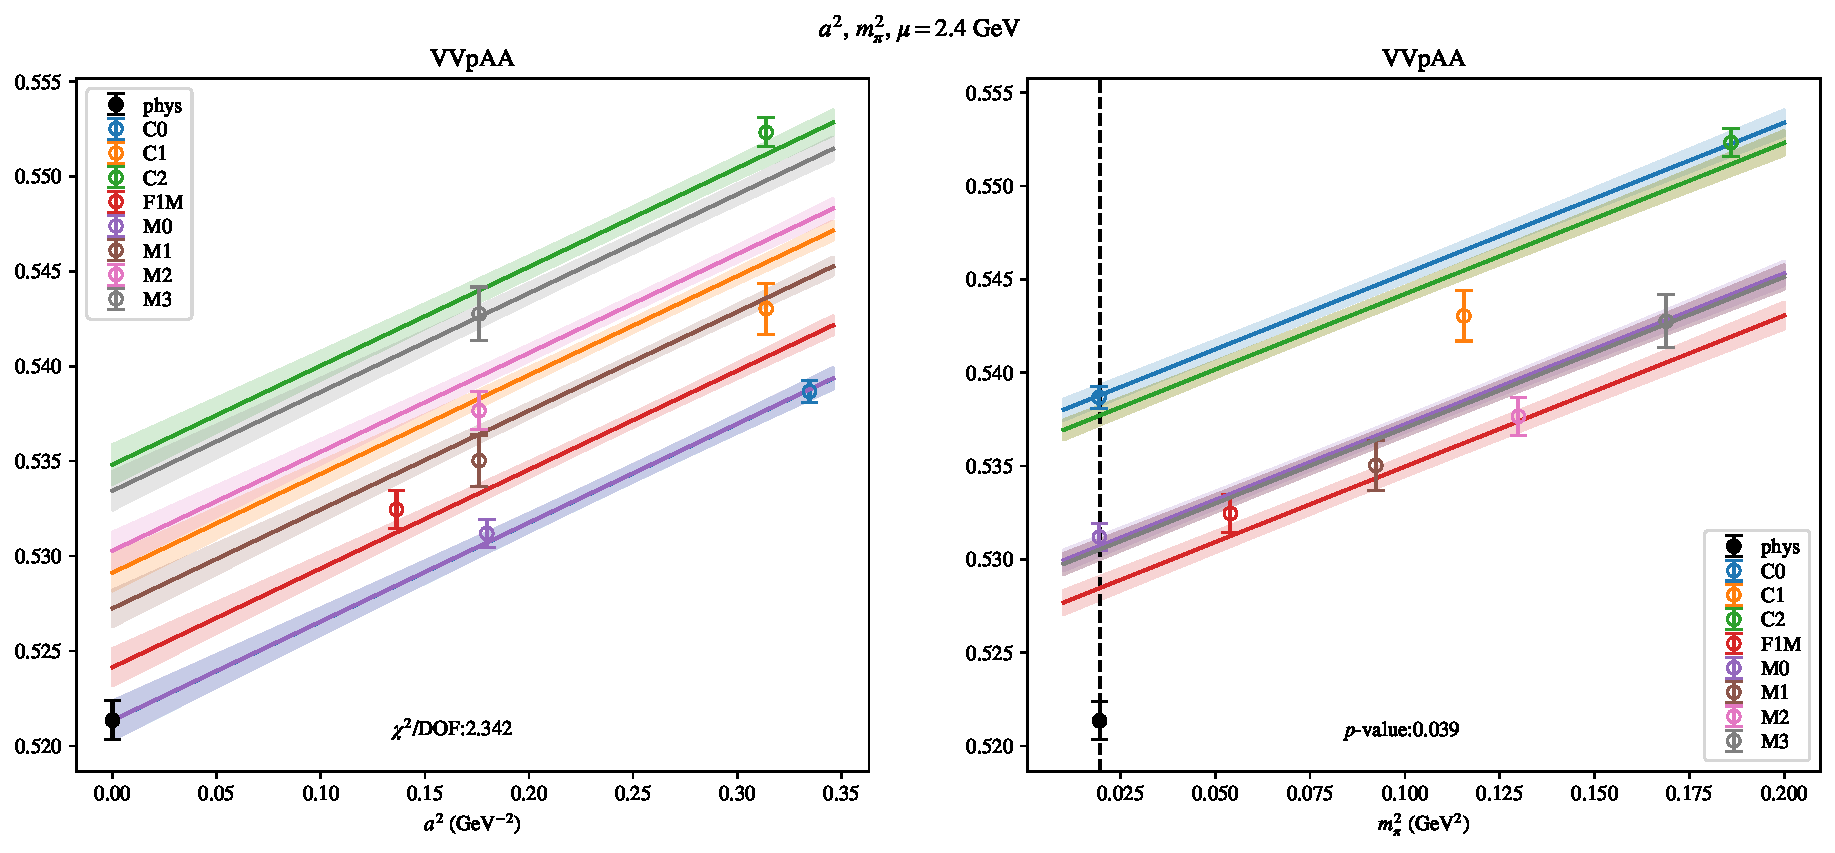
\includepdf[link, pages=-]{VVpAA/a2m2_24.pdf}
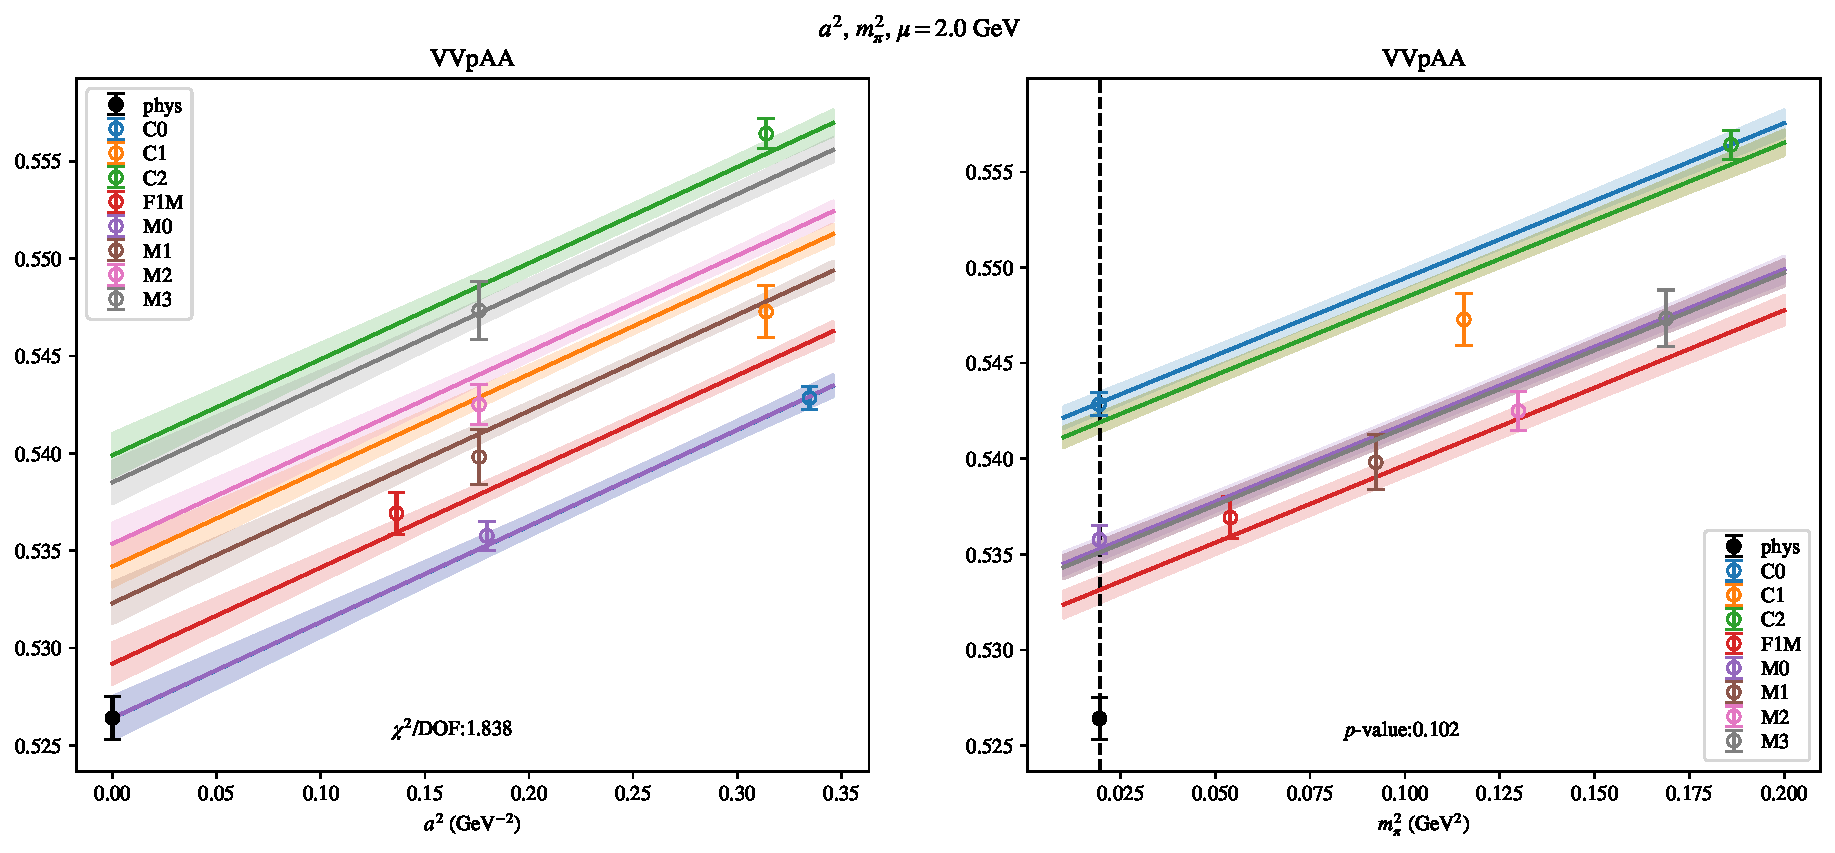
\includepdf[link, pages=-]{VVpAA/a2m2_20.pdf}
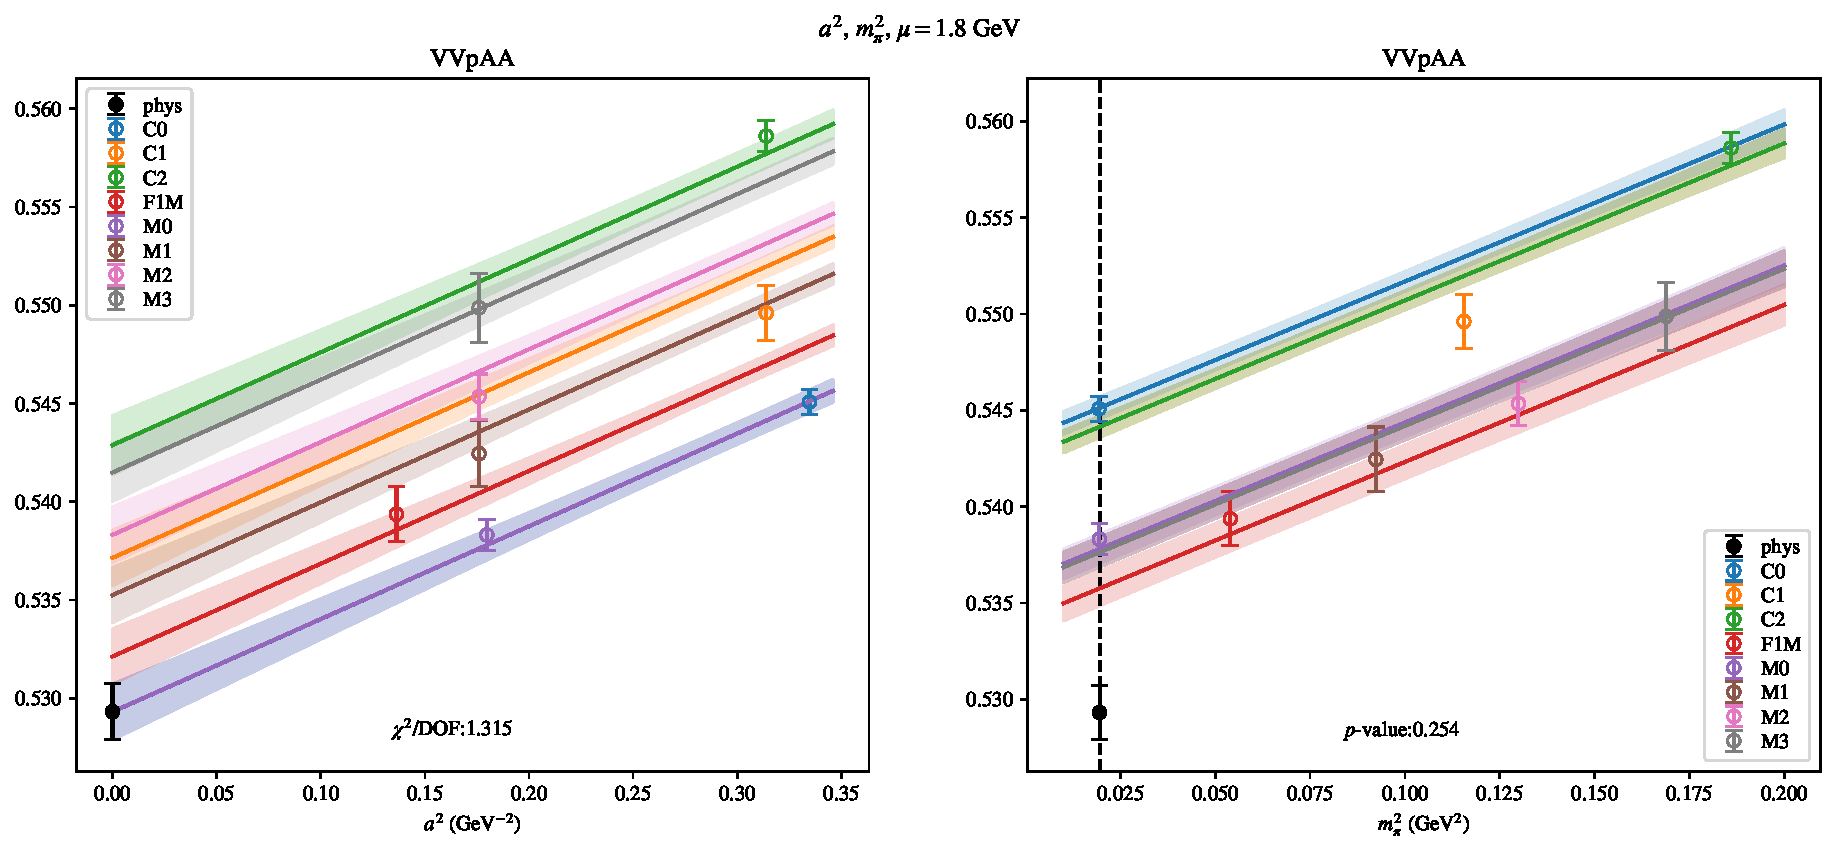
\includepdf[link, pages=-]{VVpAA/a2m2_18.pdf}
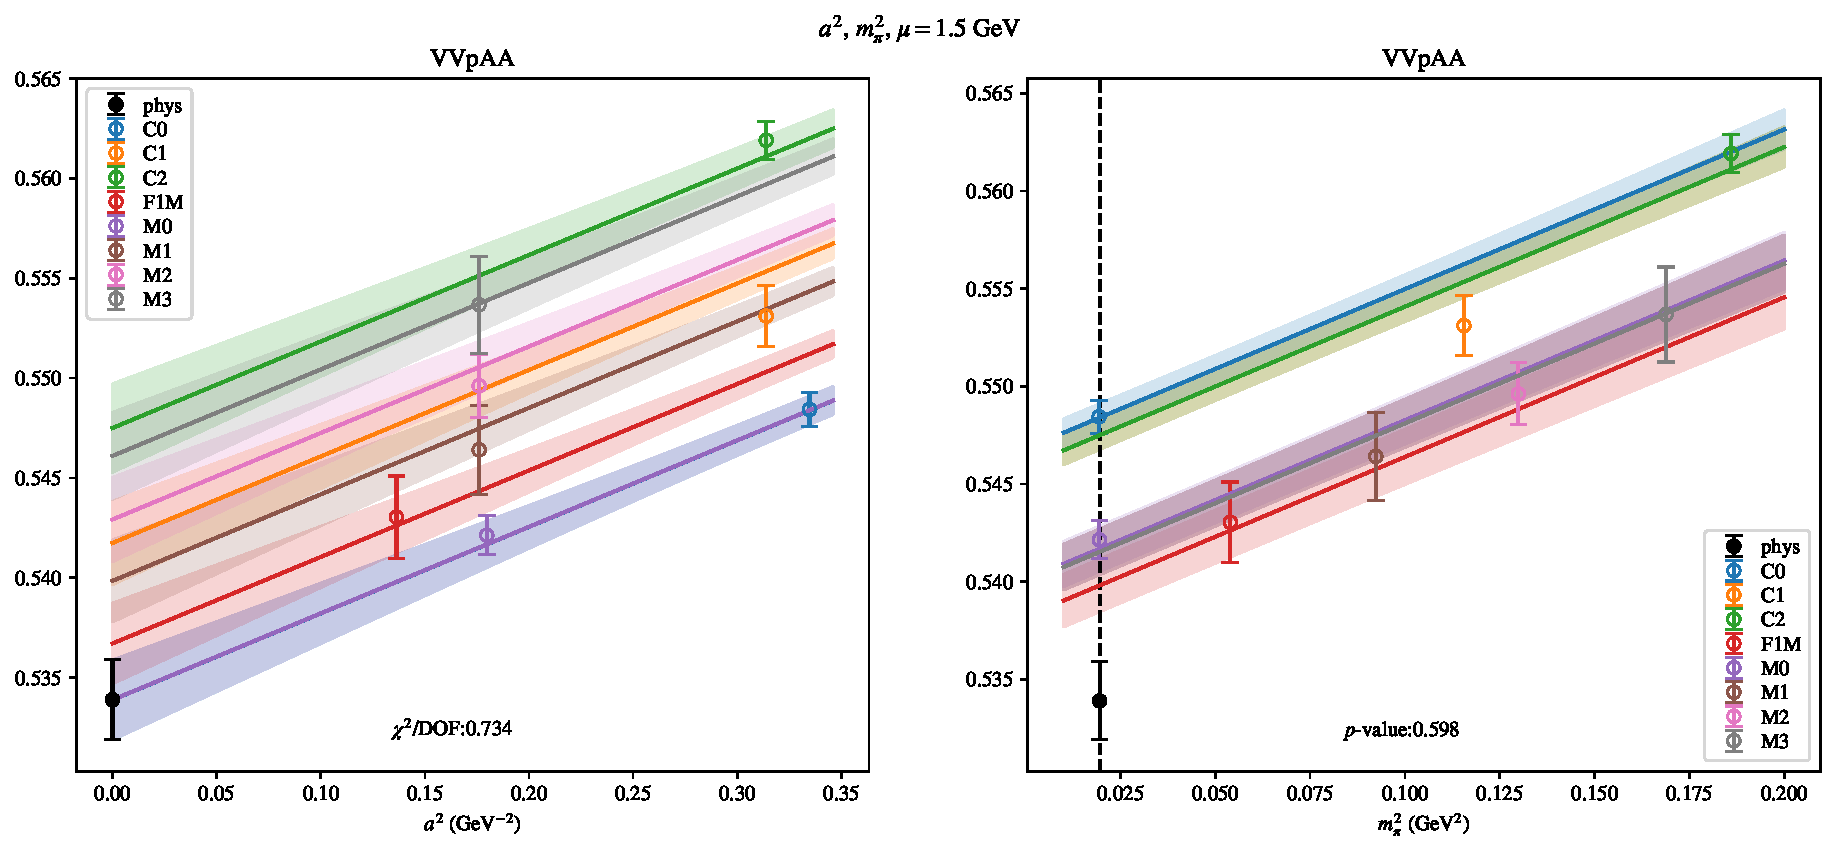
\includepdf[link, pages=-]{VVpAA/a2m2_15.pdf}
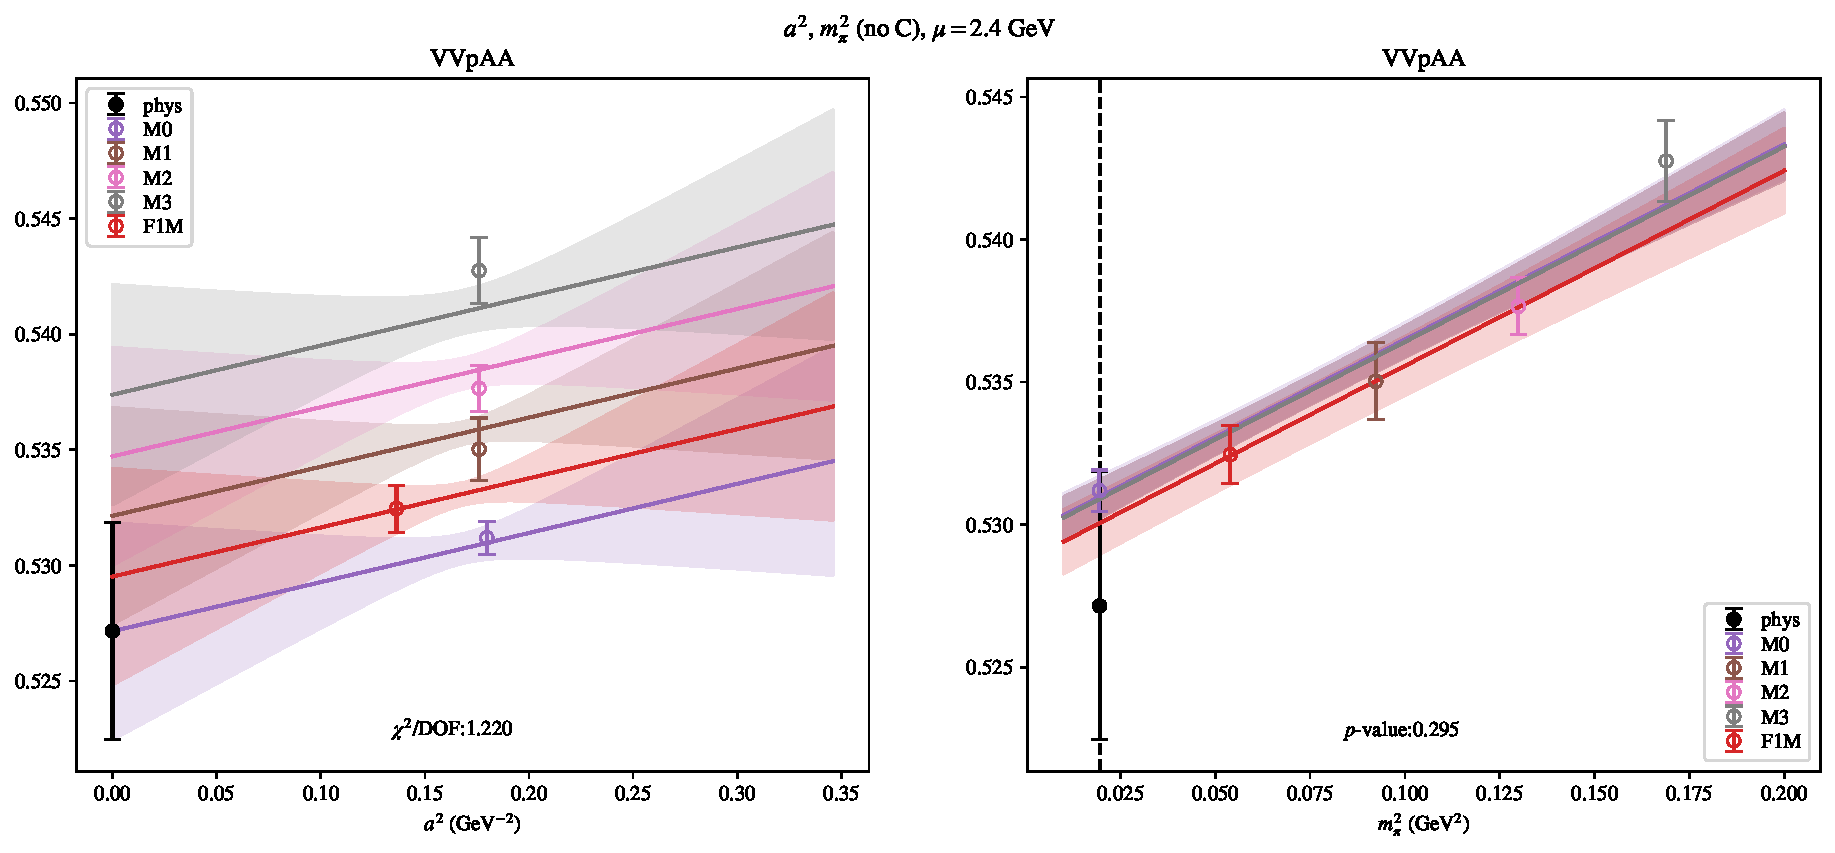
\includepdf[link, pages=-]{VVpAA/a2m2noC_24.pdf}
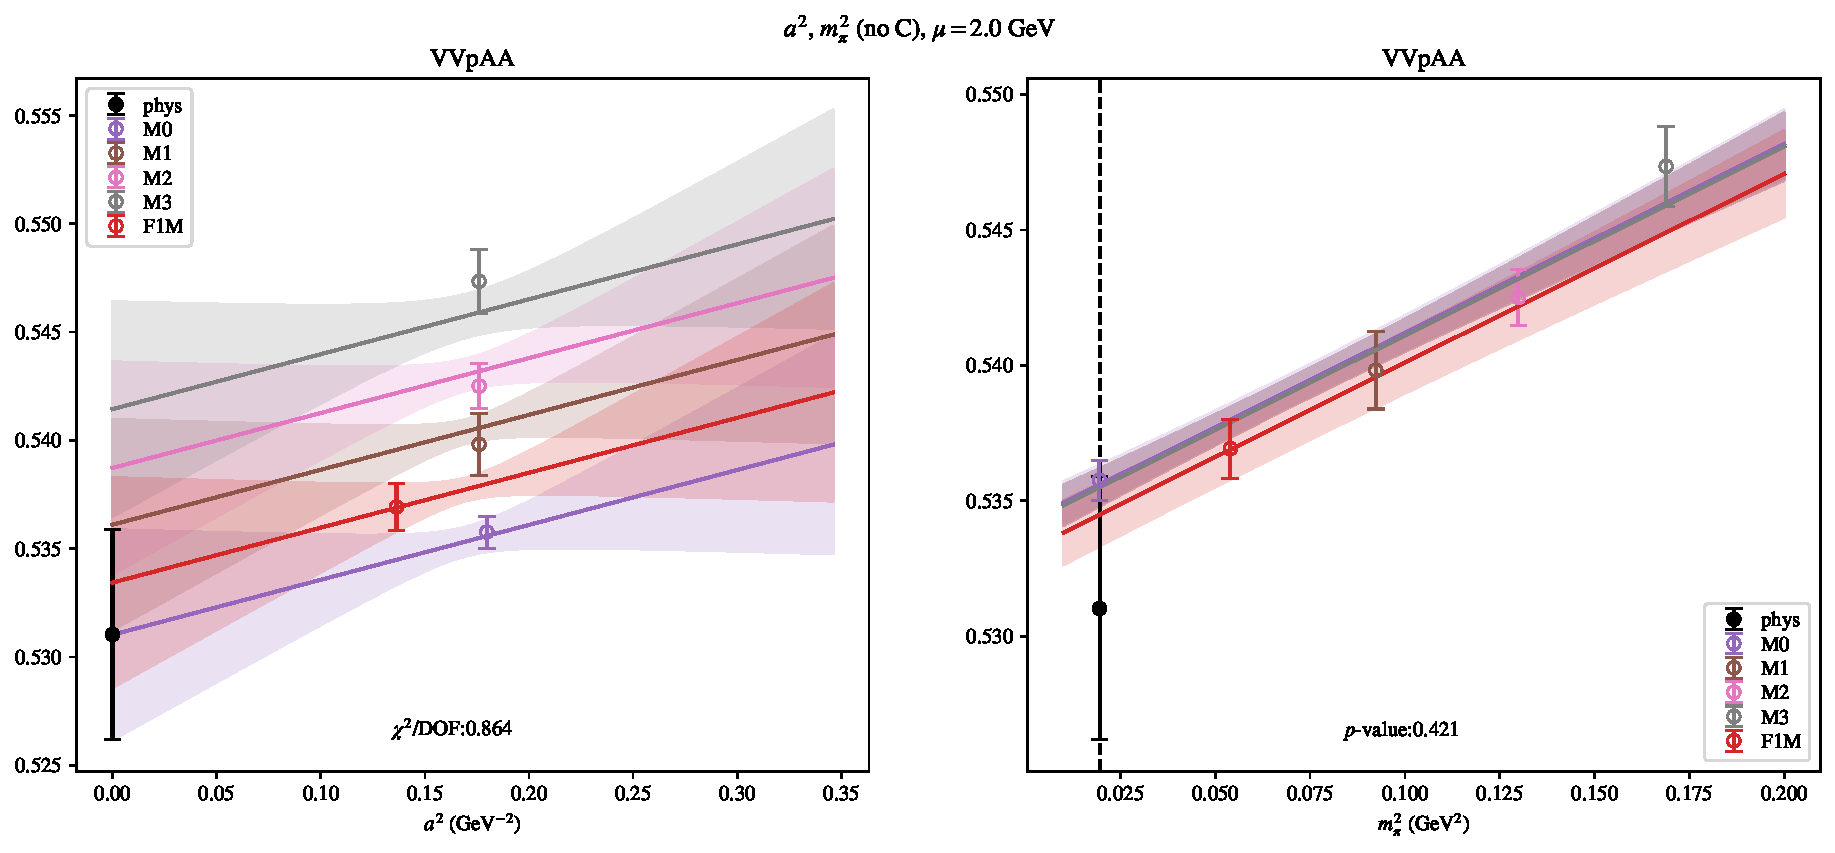
\includepdf[link, pages=-]{VVpAA/a2m2noC_20.pdf}
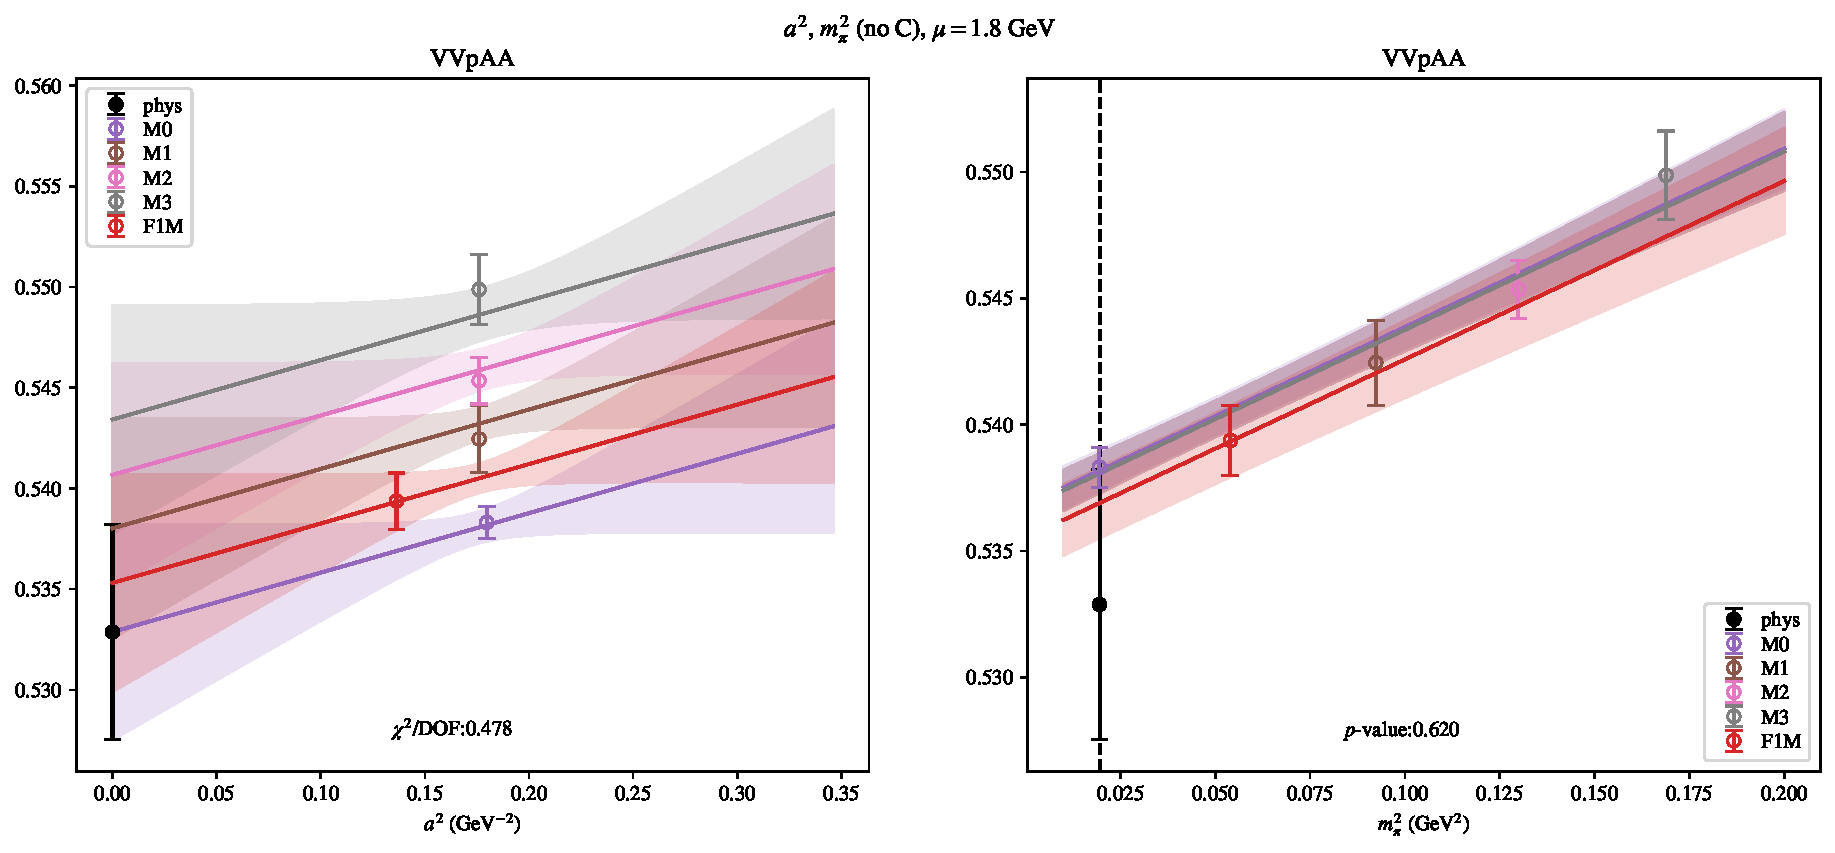
\includepdf[link, pages=-]{VVpAA/a2m2noC_18.pdf}
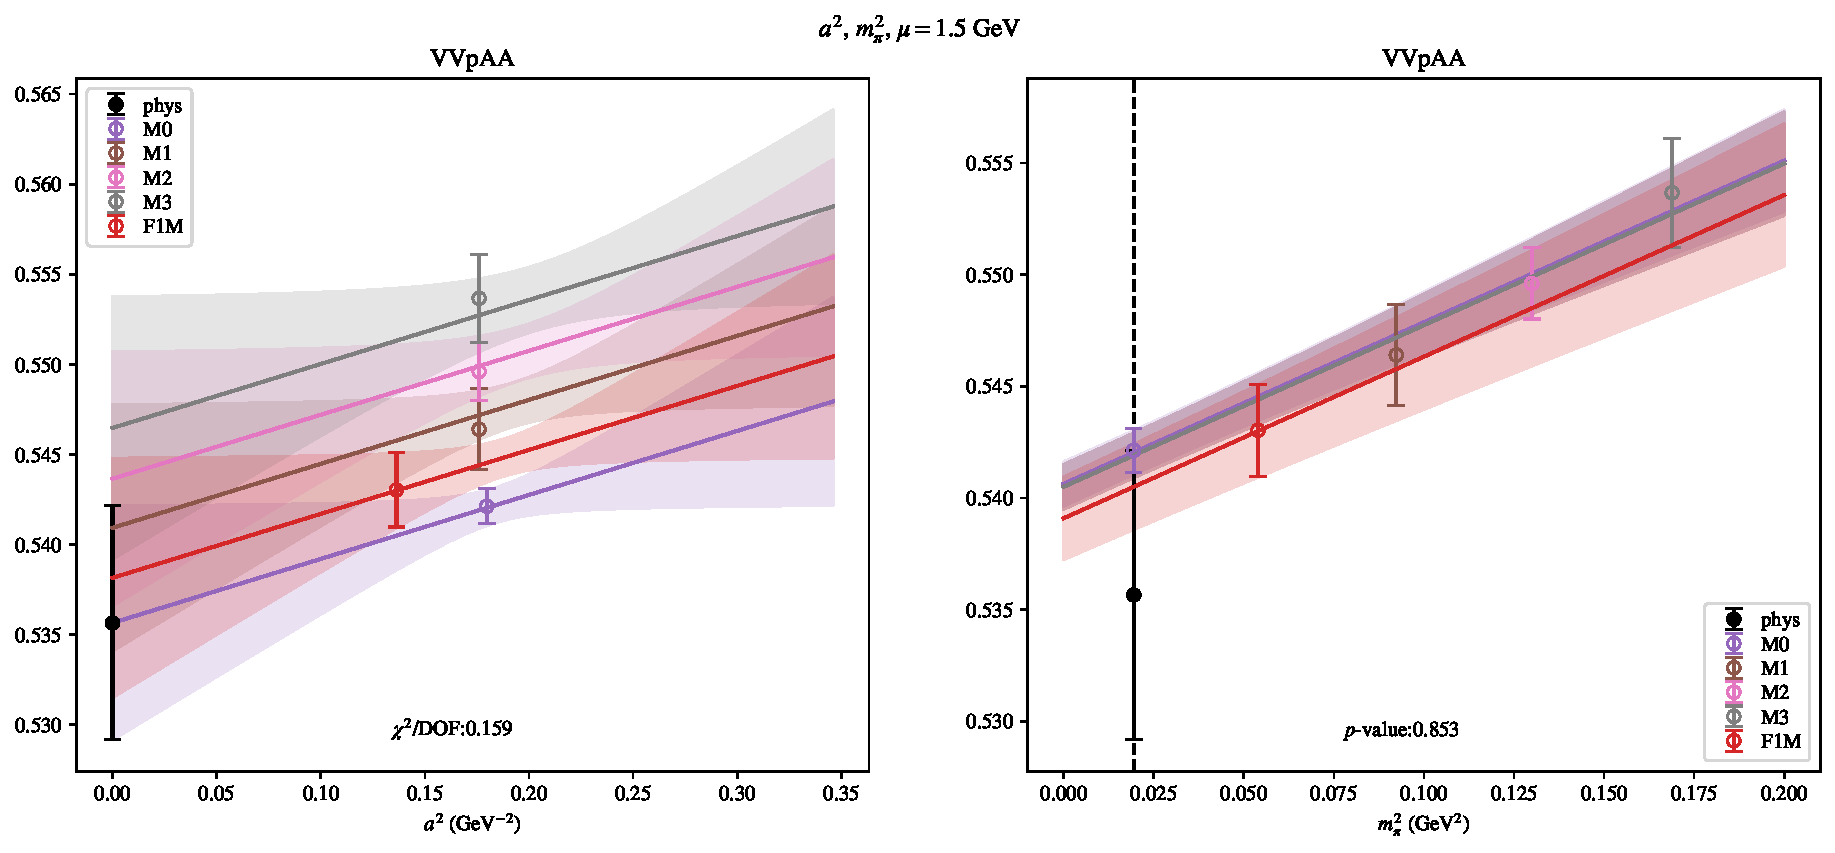
\includepdf[link, pages=-]{VVpAA/a2m2noC_15.pdf}
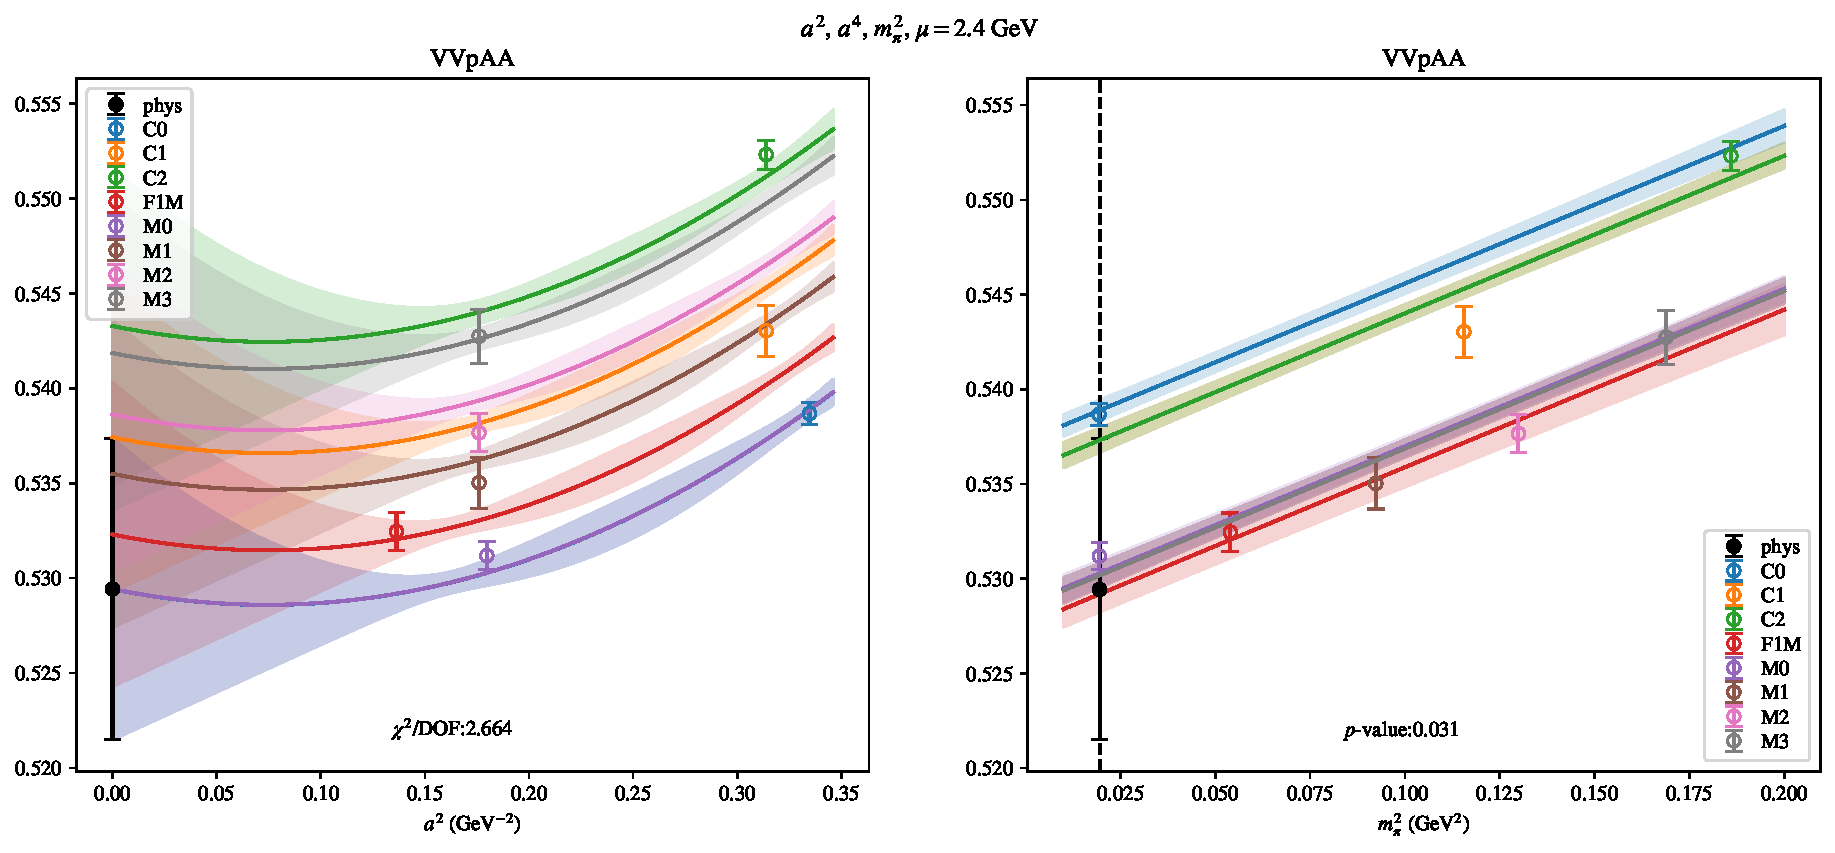
\includepdf[link, pages=-]{VVpAA/a2a4m2_24.pdf}
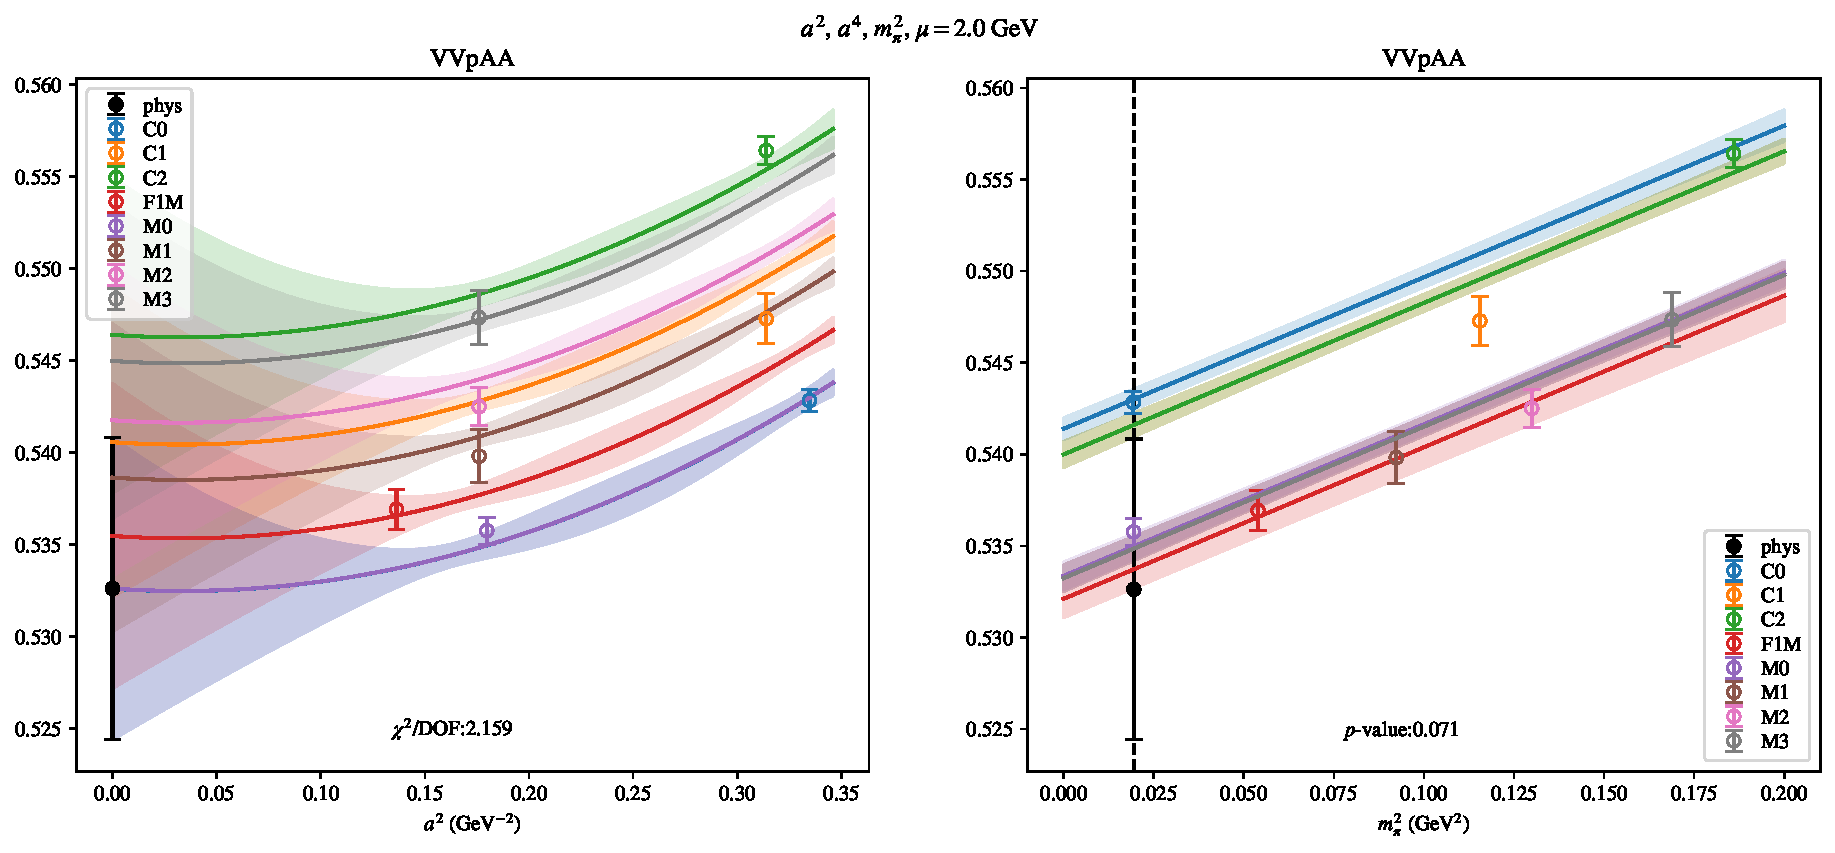
\includepdf[link, pages=-]{VVpAA/a2a4m2_20.pdf}
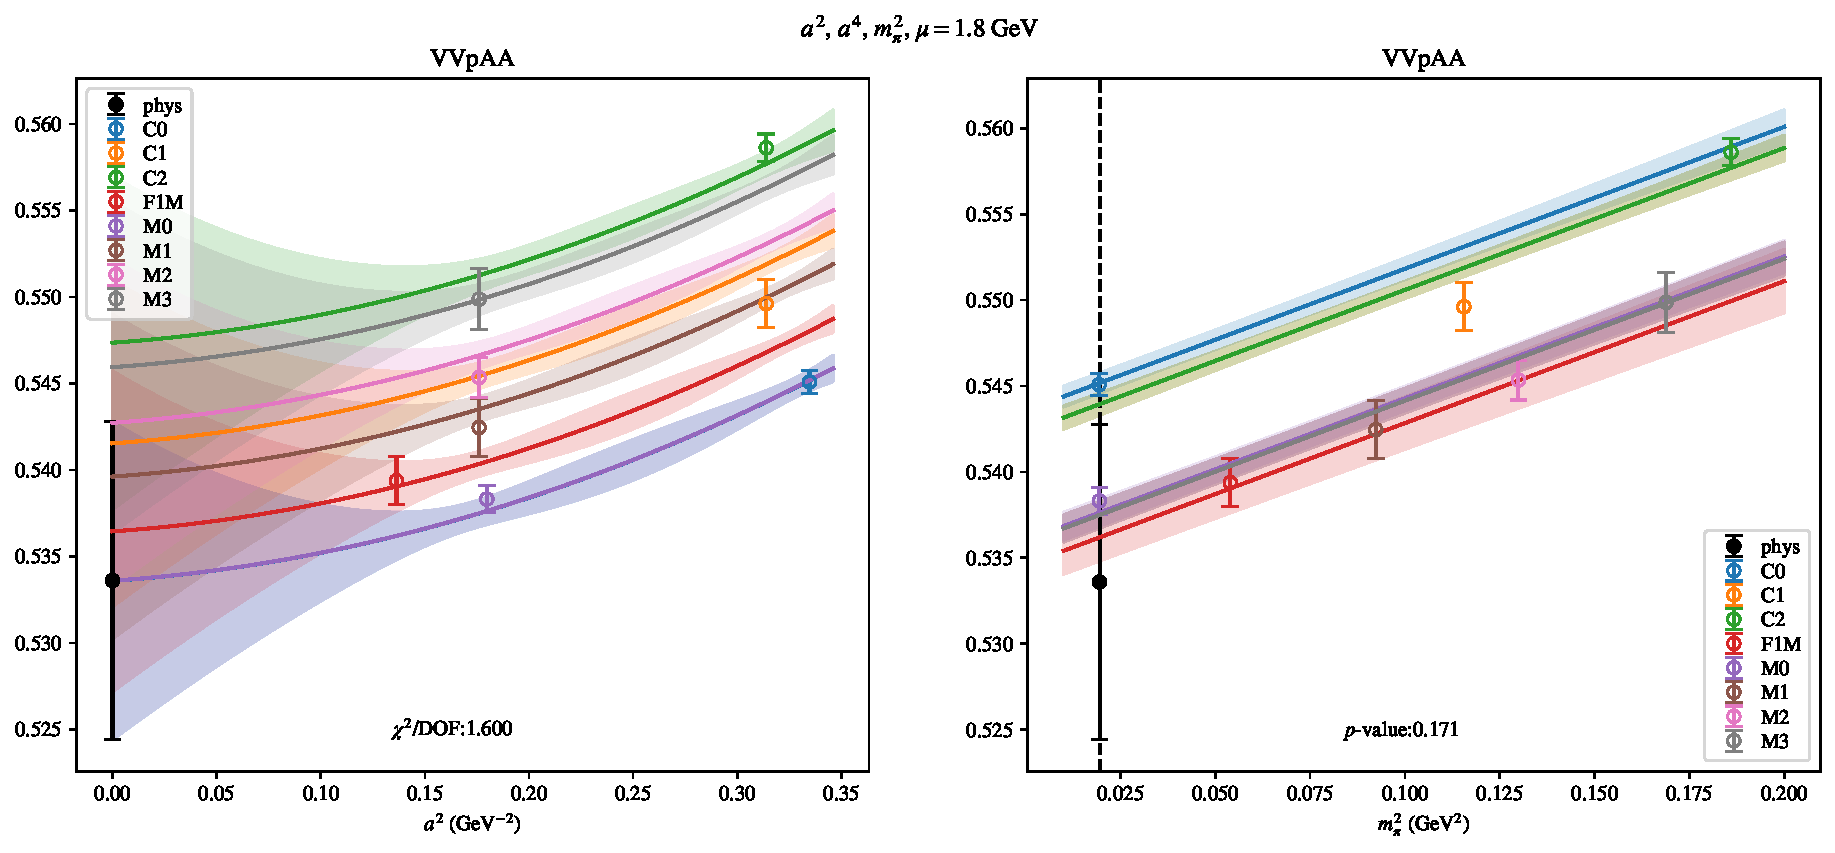
\includepdf[link, pages=-]{VVpAA/a2a4m2_18.pdf}
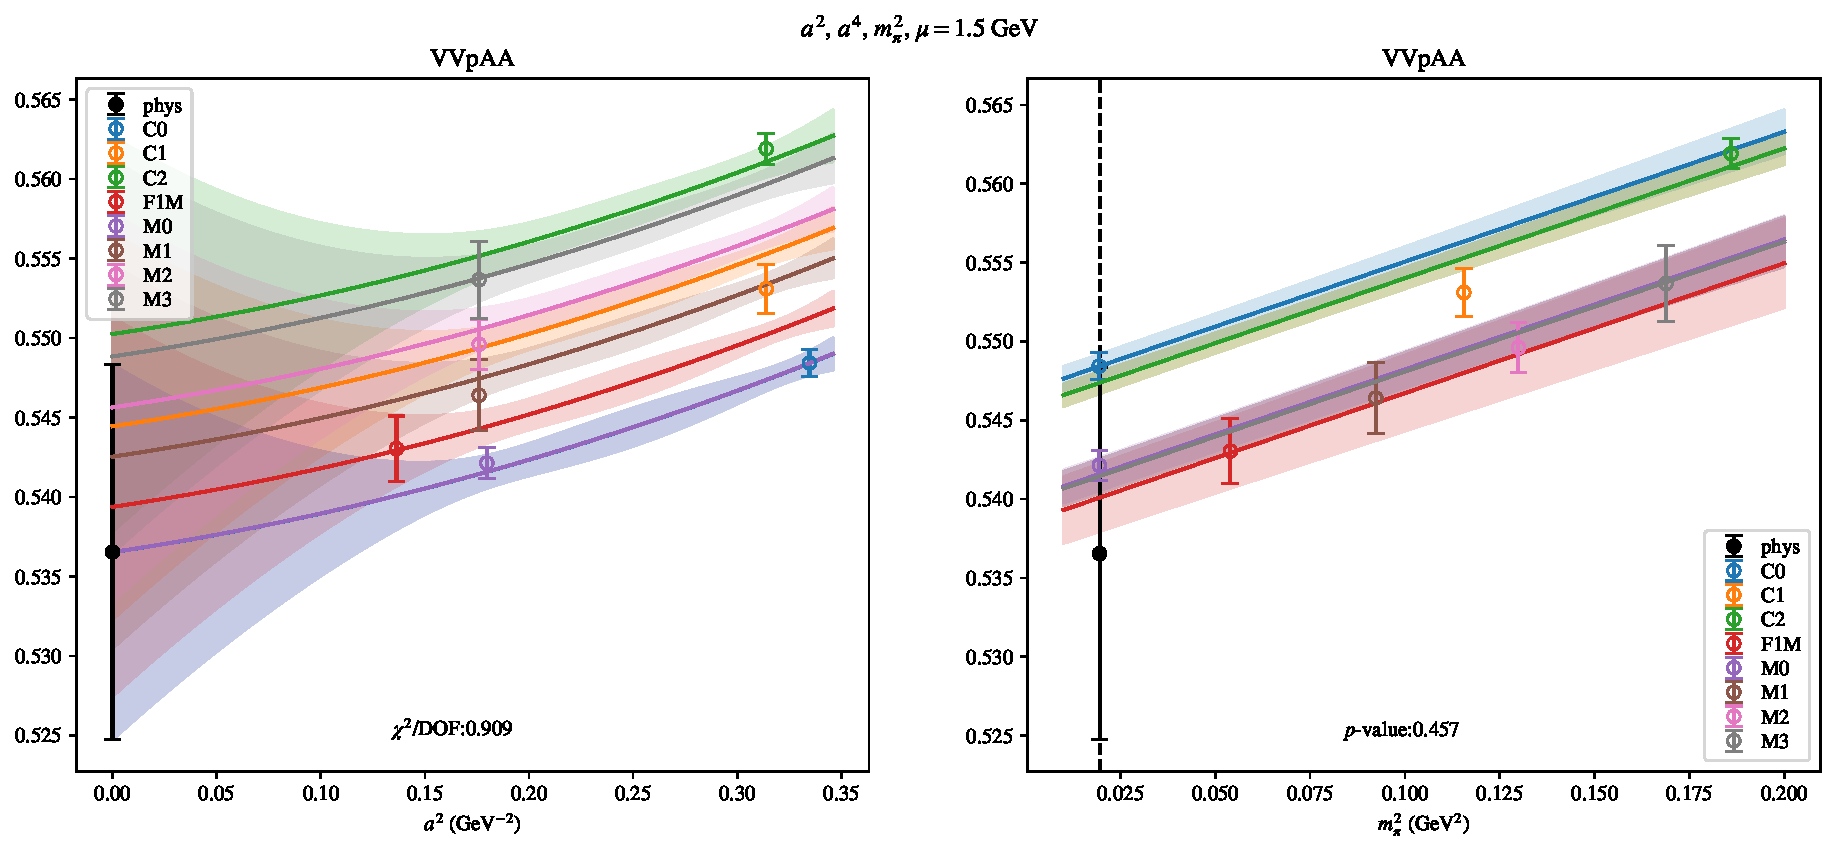
\includepdf[link, pages=-]{VVpAA/a2a4m2_15.pdf}
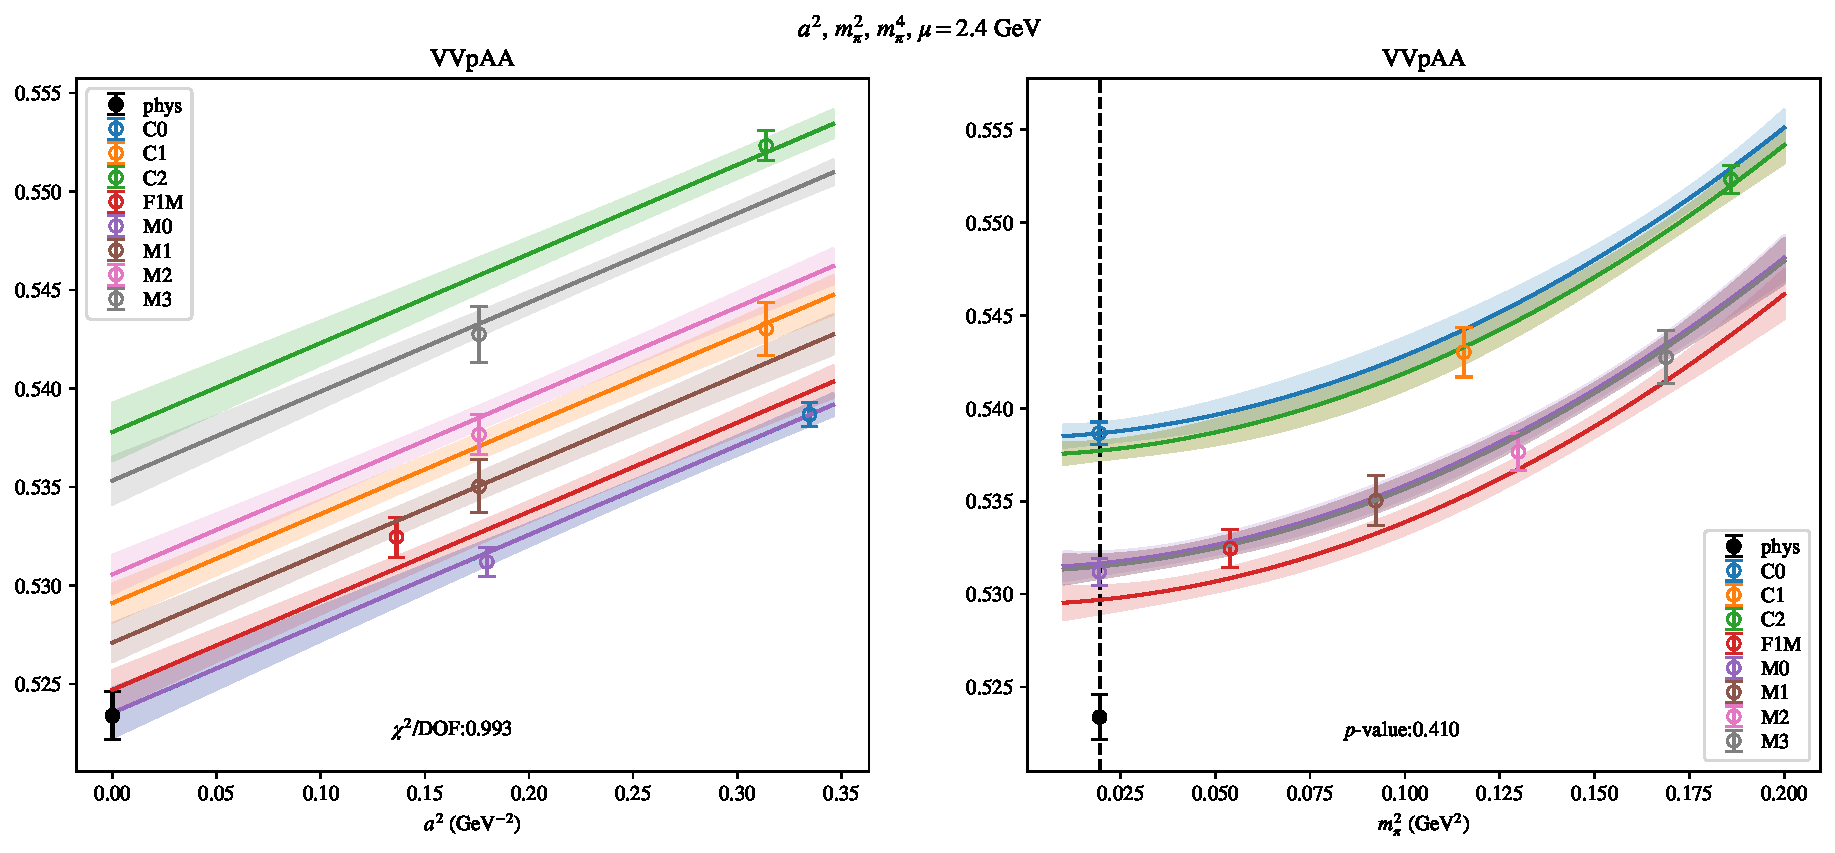
\includepdf[link, pages=-]{VVpAA/a2m2m4_24.pdf}
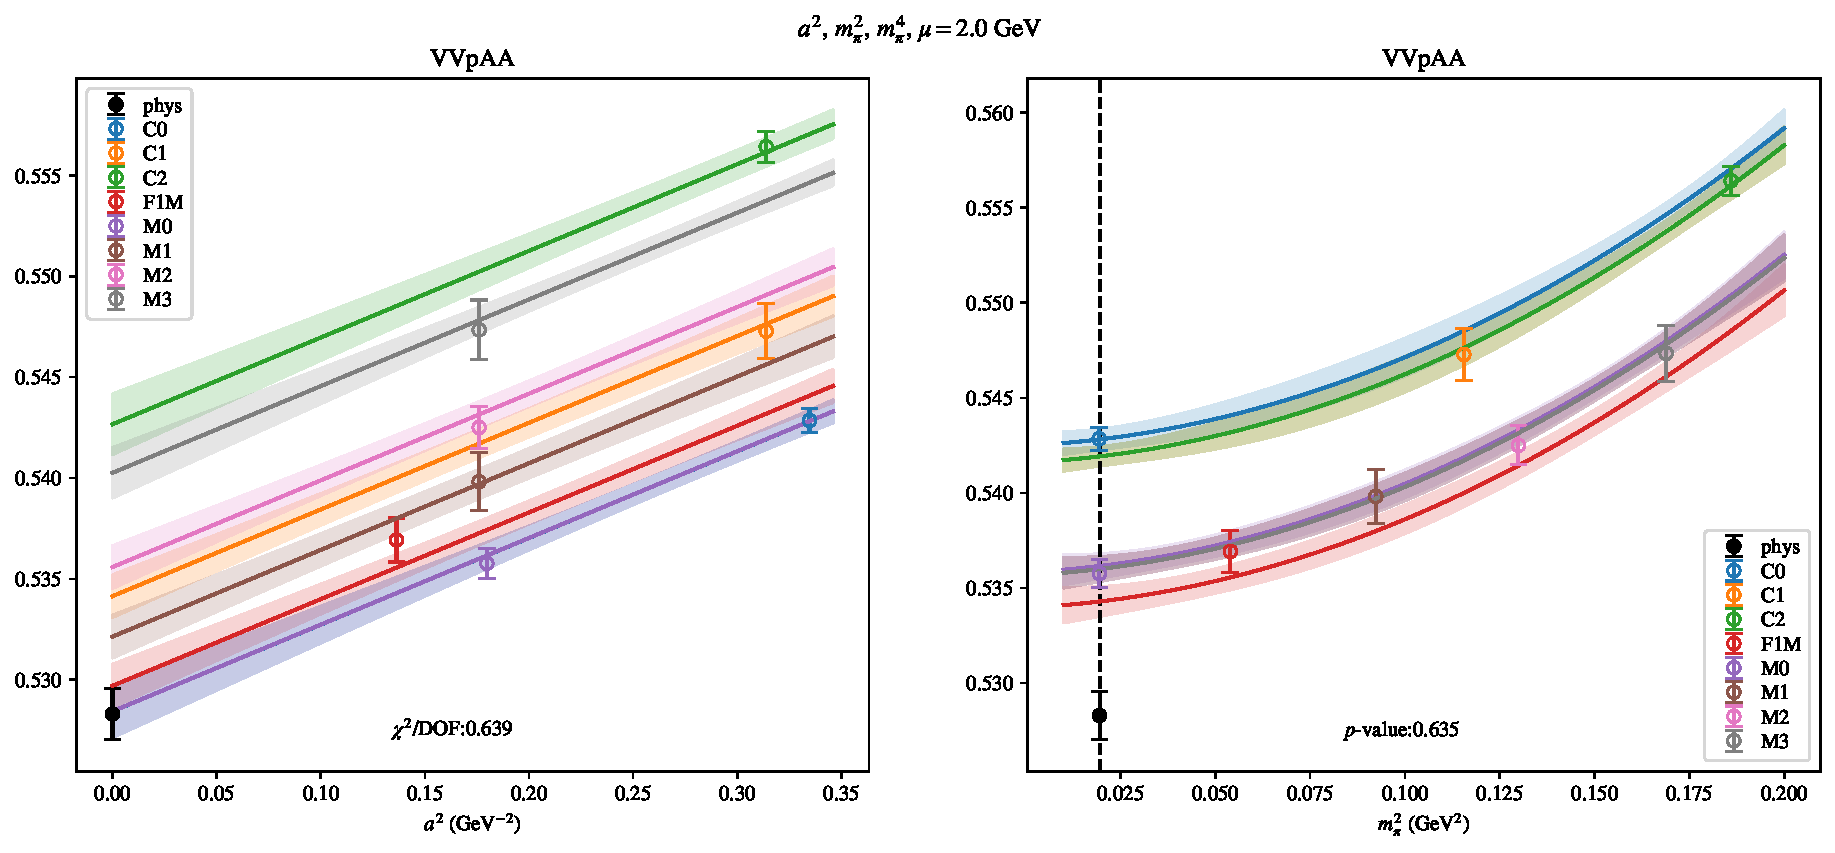
\includepdf[link, pages=-]{VVpAA/a2m2m4_20.pdf}
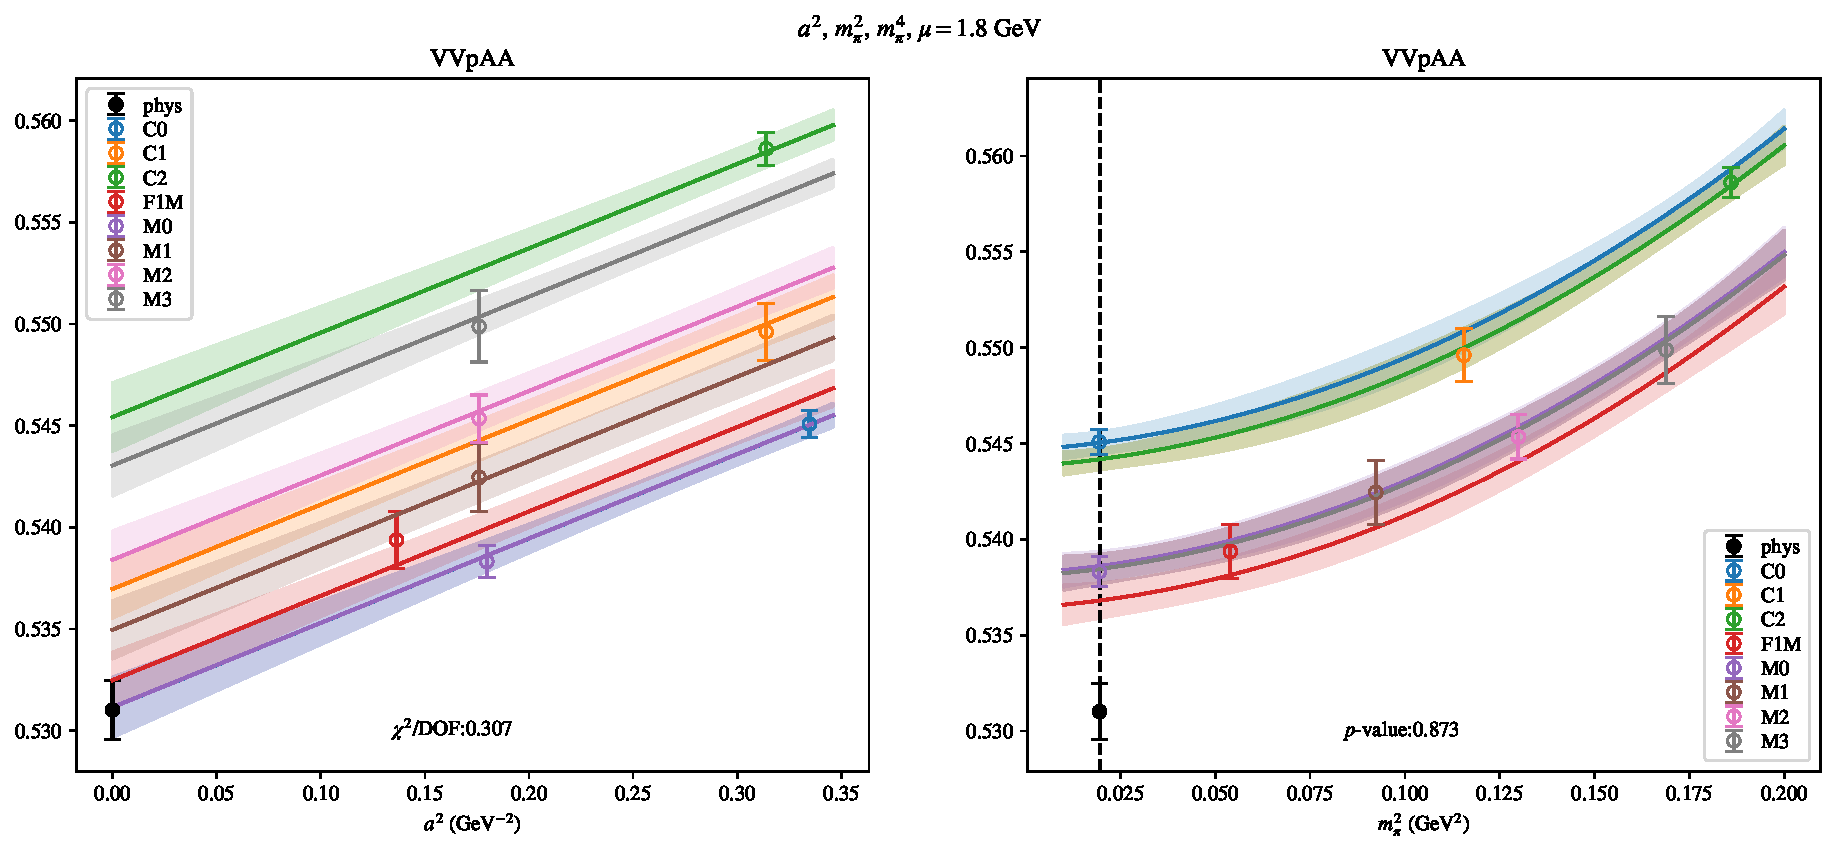
\includepdf[link, pages=-]{VVpAA/a2m2m4_18.pdf}
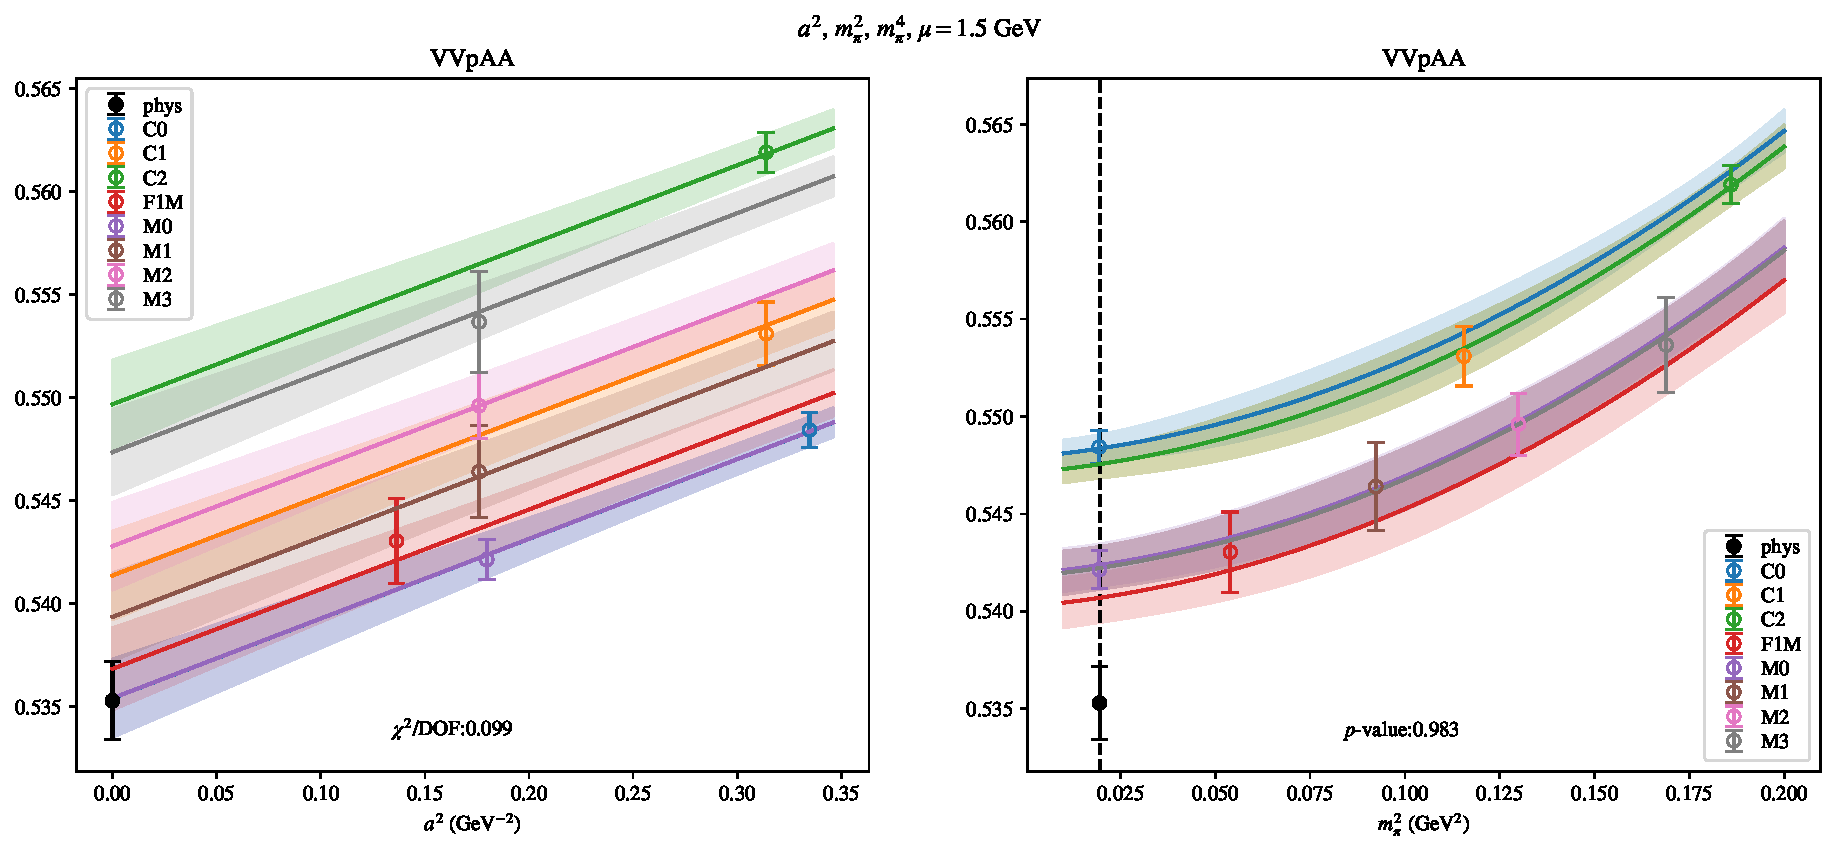
\includepdf[link, pages=-]{VVpAA/a2m2m4_15.pdf}
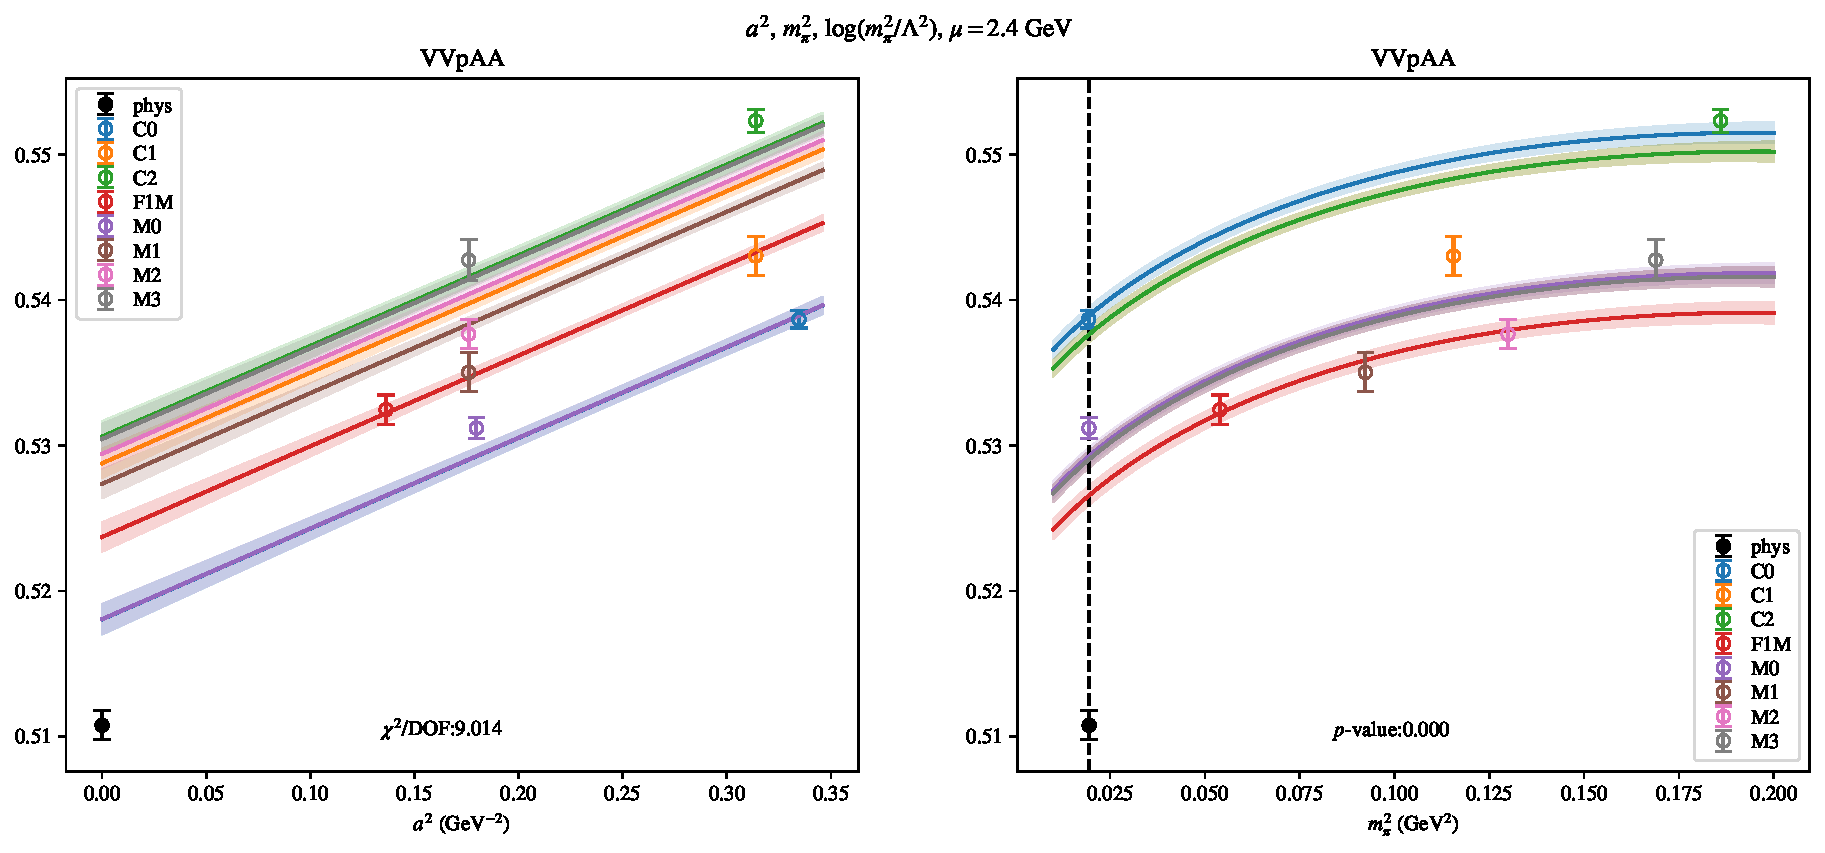
\includepdf[link, pages=-]{VVpAA/a2m2logm2_24.pdf}
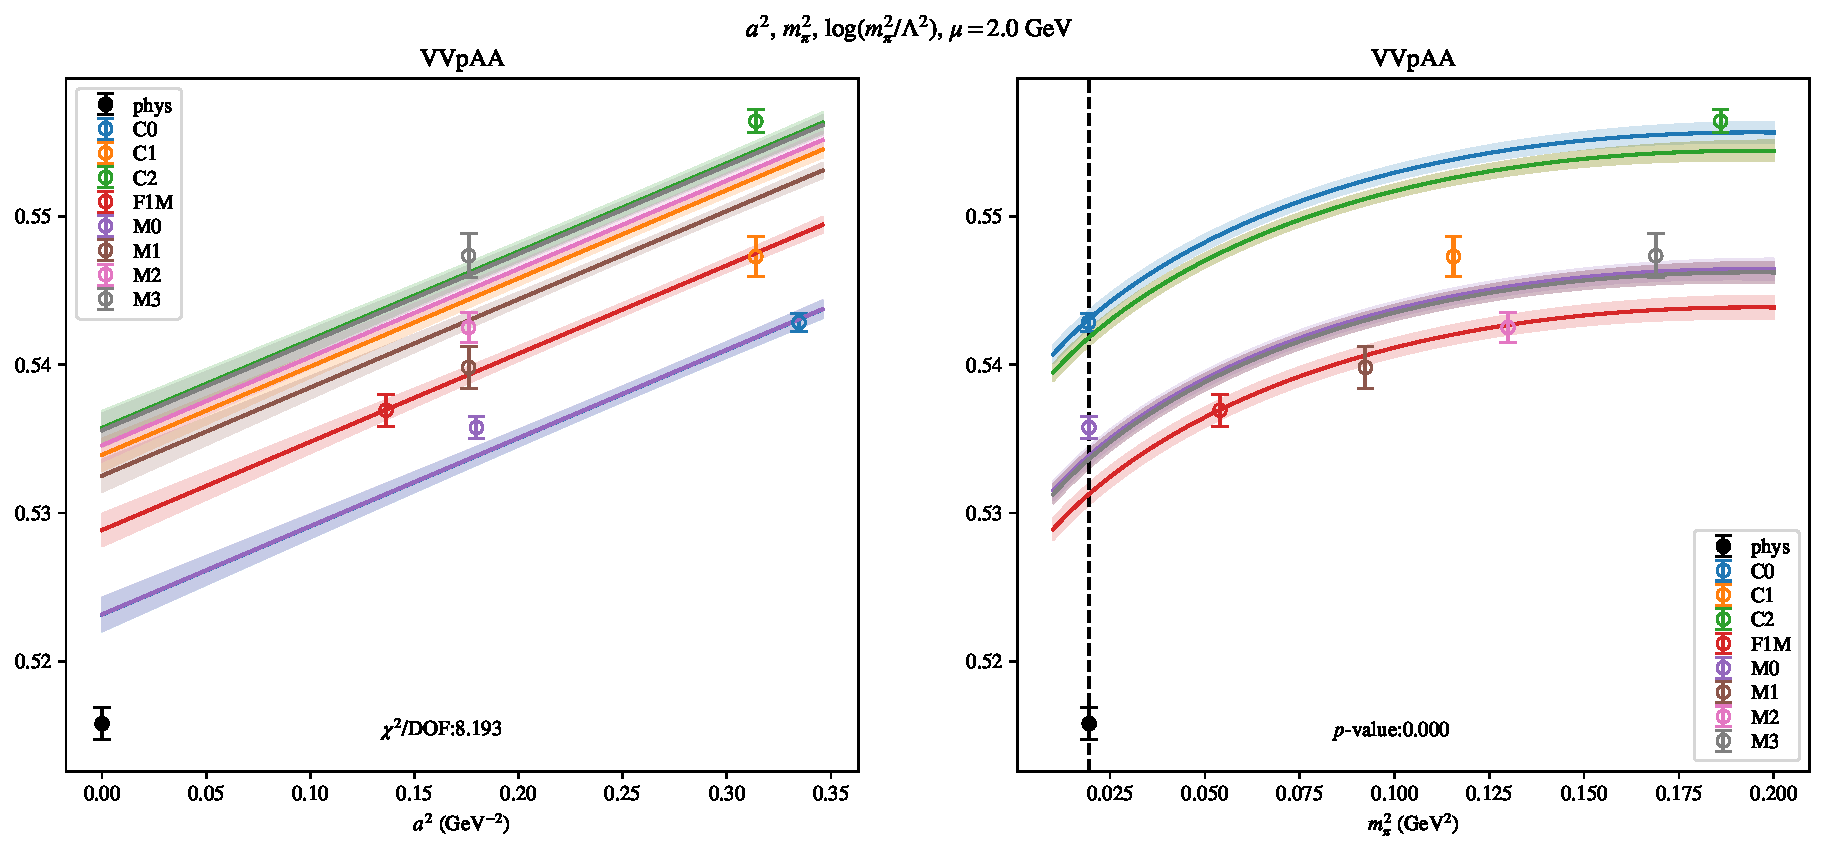
\includepdf[link, pages=-]{VVpAA/a2m2logm2_20.pdf}
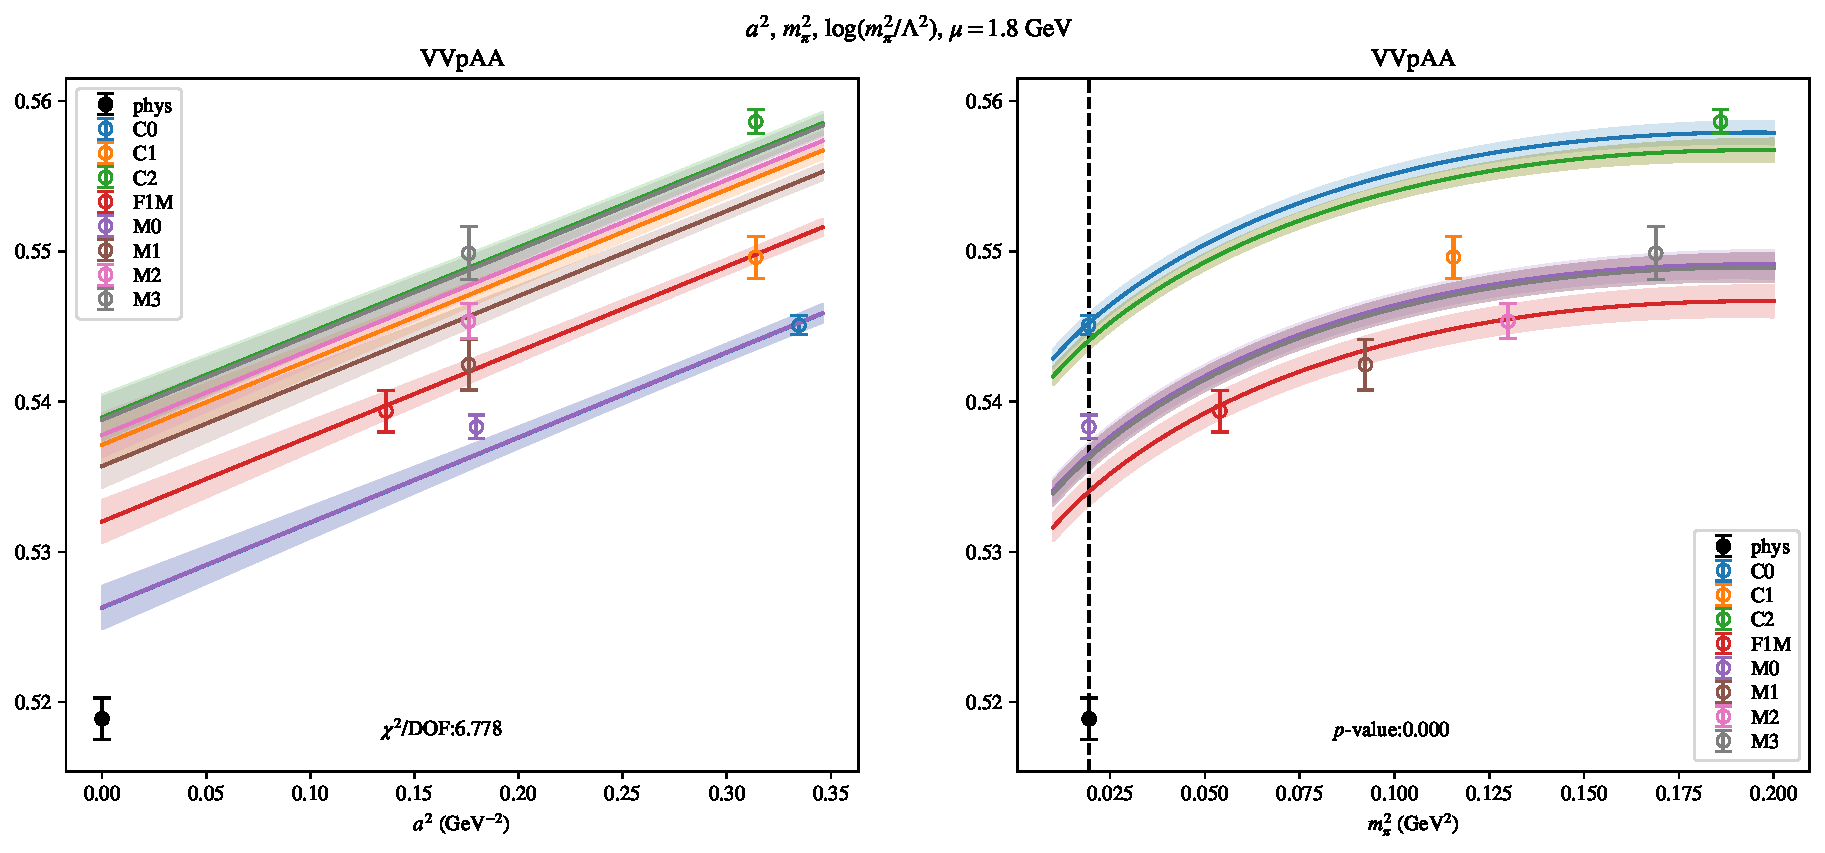
\includepdf[link, pages=-]{VVpAA/a2m2logm2_18.pdf}
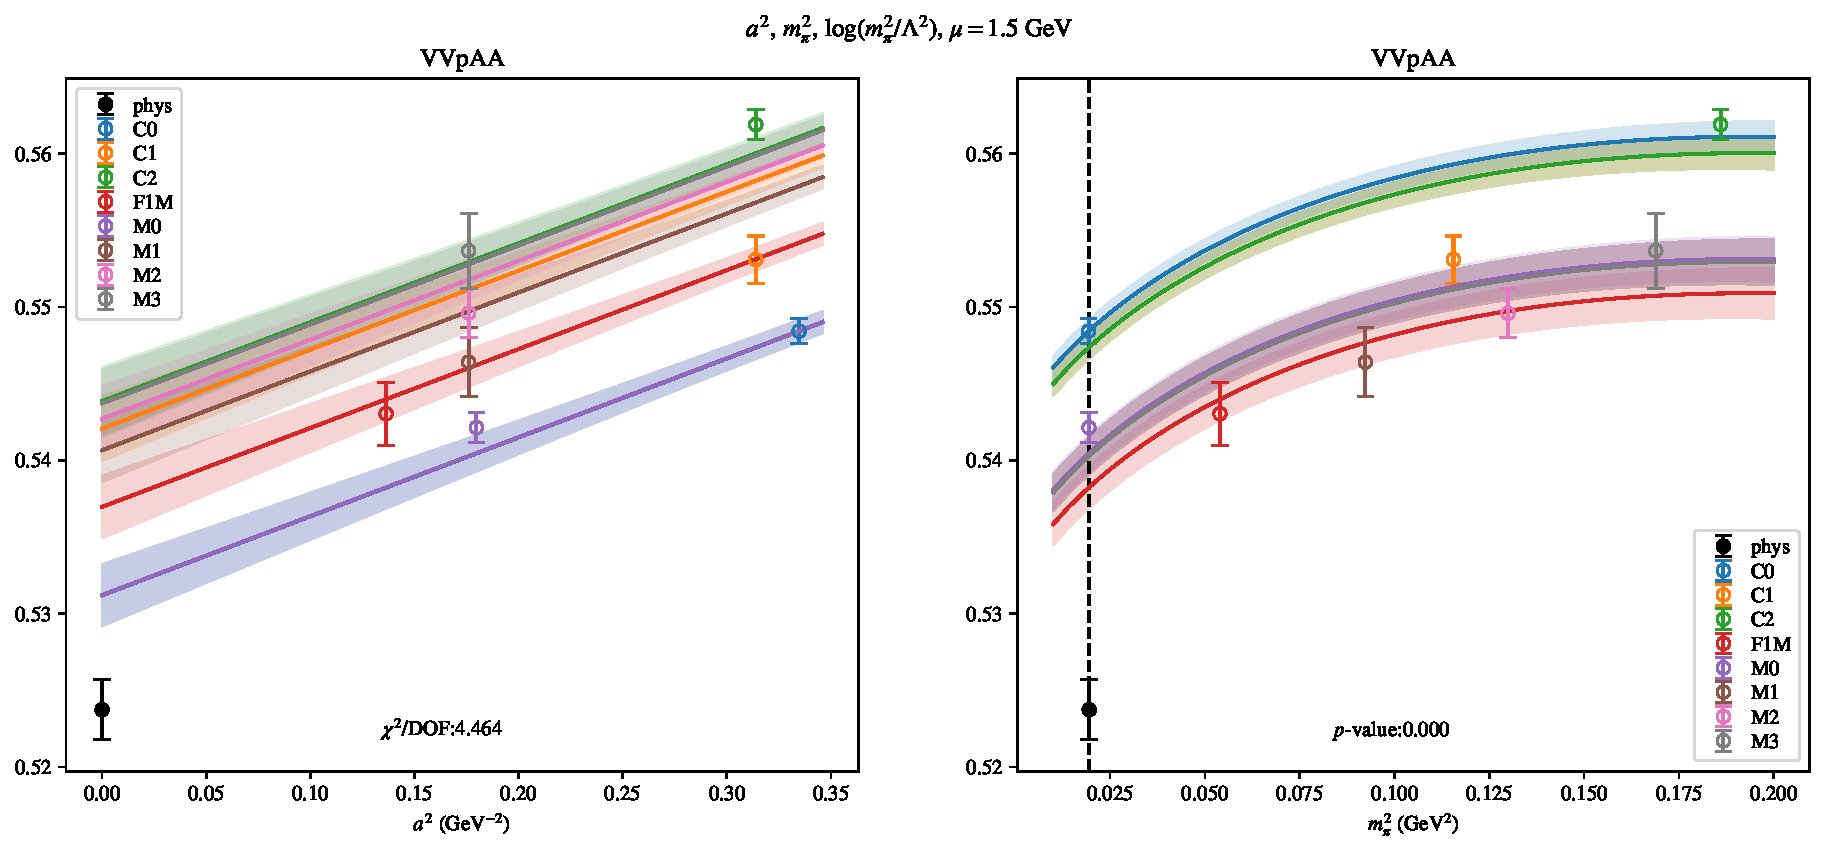
\includepdf[link, pages=-]{VVpAA/a2m2logm2_15.pdf}
\clearpage
\section{$B_2$}
\begin{table}[h!]
\begin{center}
\begin{tabular}{|c|c|c|c|c|c|}
\hline
$\mu$ (GeV) & $a^2$, $m_\pi^2$& $a^2$, $m_\pi^2$ (no C)& $a^2$, $a^4$, $m_\pi^2$& $a^2$, $m_\pi^2$, $m_\pi^4$& $a^2$, $m_\pi^2$, $\log(m_\pi^2/\Lambda^2)$\\
\hline
2.4& \hyperlink{VVmAA/a2m2_24.pdf.1}{\textbf{0.53833(89)}: 5.538 (0.0)} & \hyperlink{VVmAA/a2m2noC_24.pdf.1}{\textbf{0.5585(52)}: 1.377 (0.252)} & \hyperlink{VVmAA/a2a4m2_24.pdf.1}{\textbf{0.5565(86)}: 5.756 (0.0)} & \hyperlink{VVmAA/a2m2m4_24.pdf.1}{\textbf{0.53751(95)}: 5.517 (0.0)} & \hyperlink{VVmAA/a2m2logm2_24.pdf.1}{\textbf{0.52896(88)}: 4.379 (0.001)}\\
2.0& \hyperlink{VVmAA/a2m2_20.pdf.1}{\textbf{0.56754(98)}: 4.716 (0.0)} & \hyperlink{VVmAA/a2m2noC_20.pdf.1}{\textbf{0.5922(55)}: 0.797 (0.451)} & \hyperlink{VVmAA/a2a4m2_20.pdf.1}{\textbf{0.5969(91)}: 3.427 (0.008)} & \hyperlink{VVmAA/a2m2m4_20.pdf.1}{\textbf{0.5666(10)}: 4.48 (0.001)} & \hyperlink{VVmAA/a2m2logm2_20.pdf.1}{\textbf{0.55783(96)}: 3.258 (0.006)}\\
1.8& \hyperlink{VVmAA/a2m2_18.pdf.1}{\textbf{0.5840(12)}: 3.149 (0.008)} & \hyperlink{VVmAA/a2m2noC_18.pdf.1}{\textbf{0.6114(59)}: 0.41 (0.664)} & \hyperlink{VVmAA/a2a4m2_18.pdf.1}{\textbf{0.6210(99)}: 1.37 (0.242)} & \hyperlink{VVmAA/a2m2m4_18.pdf.1}{\textbf{0.5832(11)}: 3.371 (0.009)} & \hyperlink{VVmAA/a2m2logm2_18.pdf.1}{\textbf{0.5738(11)}: 2.714 (0.019)}\\
1.5& \hyperlink{VVmAA/a2m2_15.pdf.1}{\textbf{0.6089(17)}: 1.887 (0.093)} & \hyperlink{VVmAA/a2m2noC_15.pdf.1}{\textbf{0.6400(71)}: 0.233 (0.792)} & \hyperlink{VVmAA/a2a4m2_15.pdf.1}{\textbf{0.657(12)}: 0.272 (0.896)} & \hyperlink{VVmAA/a2m2m4_15.pdf.1}{\textbf{0.6084(15)}: 2.247 (0.061)} & \hyperlink{VVmAA/a2m2logm2_15.pdf.1}{\textbf{0.5981(17)}: 2.076 (0.065)}\\
\hline
\end{tabular}
\caption{Physical point value from chiral and continuum extrapolation at renormalisation scale $\mu$. Entries are \textbf{value(error)}: $\chi^2/\text{DOF}$ ($p$-value).}
\end{center}
\end{table}
\begin{table}[h!]
\begin{center}
\begin{tabular}{|c c|c|c|c|c|c|}
\hline
$\mu$ (GeV) &  & $a^2$, $m_\pi^2$& $a^2$, $m_\pi^2$ (no C)& $a^2$, $a^4$, $m_\pi^2$& $a^2$, $m_\pi^2$, $m_\pi^4$& $a^2$, $m_\pi^2$, $\log(m_\pi^2/\Lambda^2)$\\
\hline
\multirow{2}{0.5in}{2.4} & $\alpha$ & 0.4261(69)& 0.205(56)& 0.11(14)& 0.4334(77)& 0.4427(69)\\
 & $\beta$ & 0.00765(14)& 0.00685(23)& 0.00751(15)& 0.00953(77)& 0.00297(14)\\
\hline
\multirow{2}{0.5in}{2.0} & $\alpha$ & 0.3507(67)& 0.096(54)& -0.1(13)& 0.3581(75)& 0.3654(68)\\
 & $\beta$ & 0.00799(18)& 0.00723(30)& 0.00774(17)& 0.01010(85)& 0.00327(18)\\
\hline
\multirow{2}{0.5in}{1.8} & $\alpha$ & 0.3254(70)& 0.052(56)& -0.2(13)& 0.3312(75)& 0.3409(70)\\
 & $\beta$ & 0.00812(19)& 0.00748(31)& 0.00782(18)& 0.00967(87)& 0.00338(19)\\
\hline
\multirow{2}{0.5in}{1.5} & $\alpha$ & 0.2889(77)& -0.008& -0.3(15)& 0.2926(76)& 0.3050(78)\\
 & $\beta$ & 0.00829(22)& 0.00784(37)& 0.00792(18)& 0.0092(10)& 0.00355(22)\\
\hline
\end{tabular}
\caption{Fit values of coefficients in $B = B_0(1 + \mathbf{\alpha} a^2 + \mathbf{\beta} \frac{m_\pi^2}{f_\pi^2} + \ldots)$.}
\end{center}
\end{table}
\begin{figure}
\centering
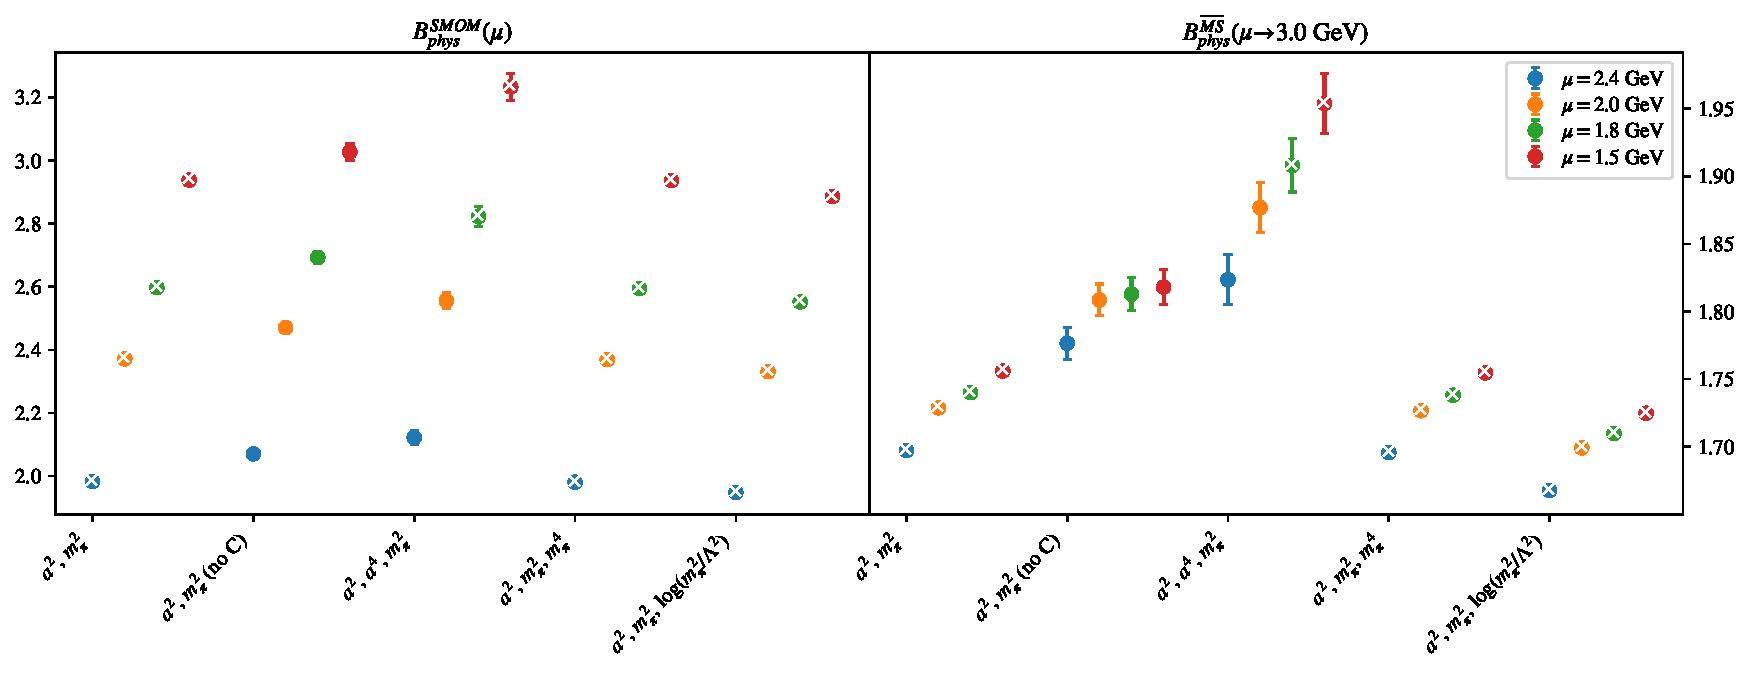
\includegraphics[page=1, width=1.1\textwidth]{plots/VVmAA_fit_summary.pdf}
\caption{\\(left) $B_{phys}$ in RI/SMOM scheme from fit variations (fits with $p$-value $<0.05$ marked with ``$\times$"). \\(right) $B_{phys}$ in $\overline{MS}$ computed using $B^{\overline{MS}} = R^{\overline{MS}\leftarrow SMOM}(3.0)\sigma_{npt}^{F1M}(3.0, 2.0) B^{SMOM}$.}
\end{figure}
\clearpage
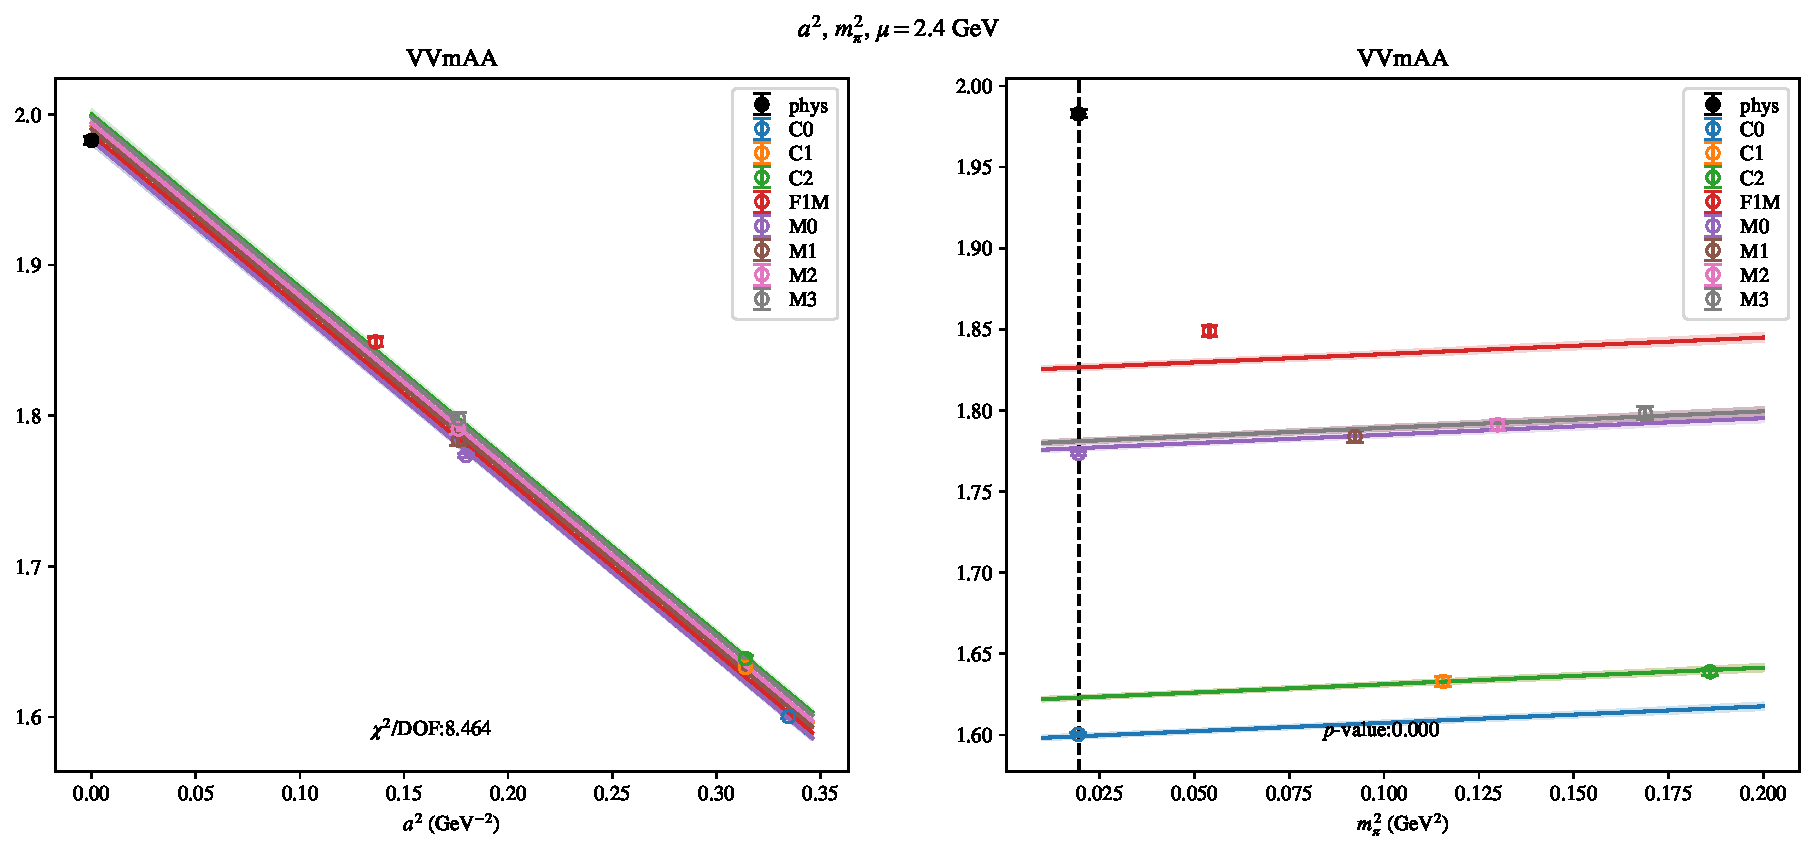
\includepdf[link, pages=-]{VVmAA/a2m2_24.pdf}
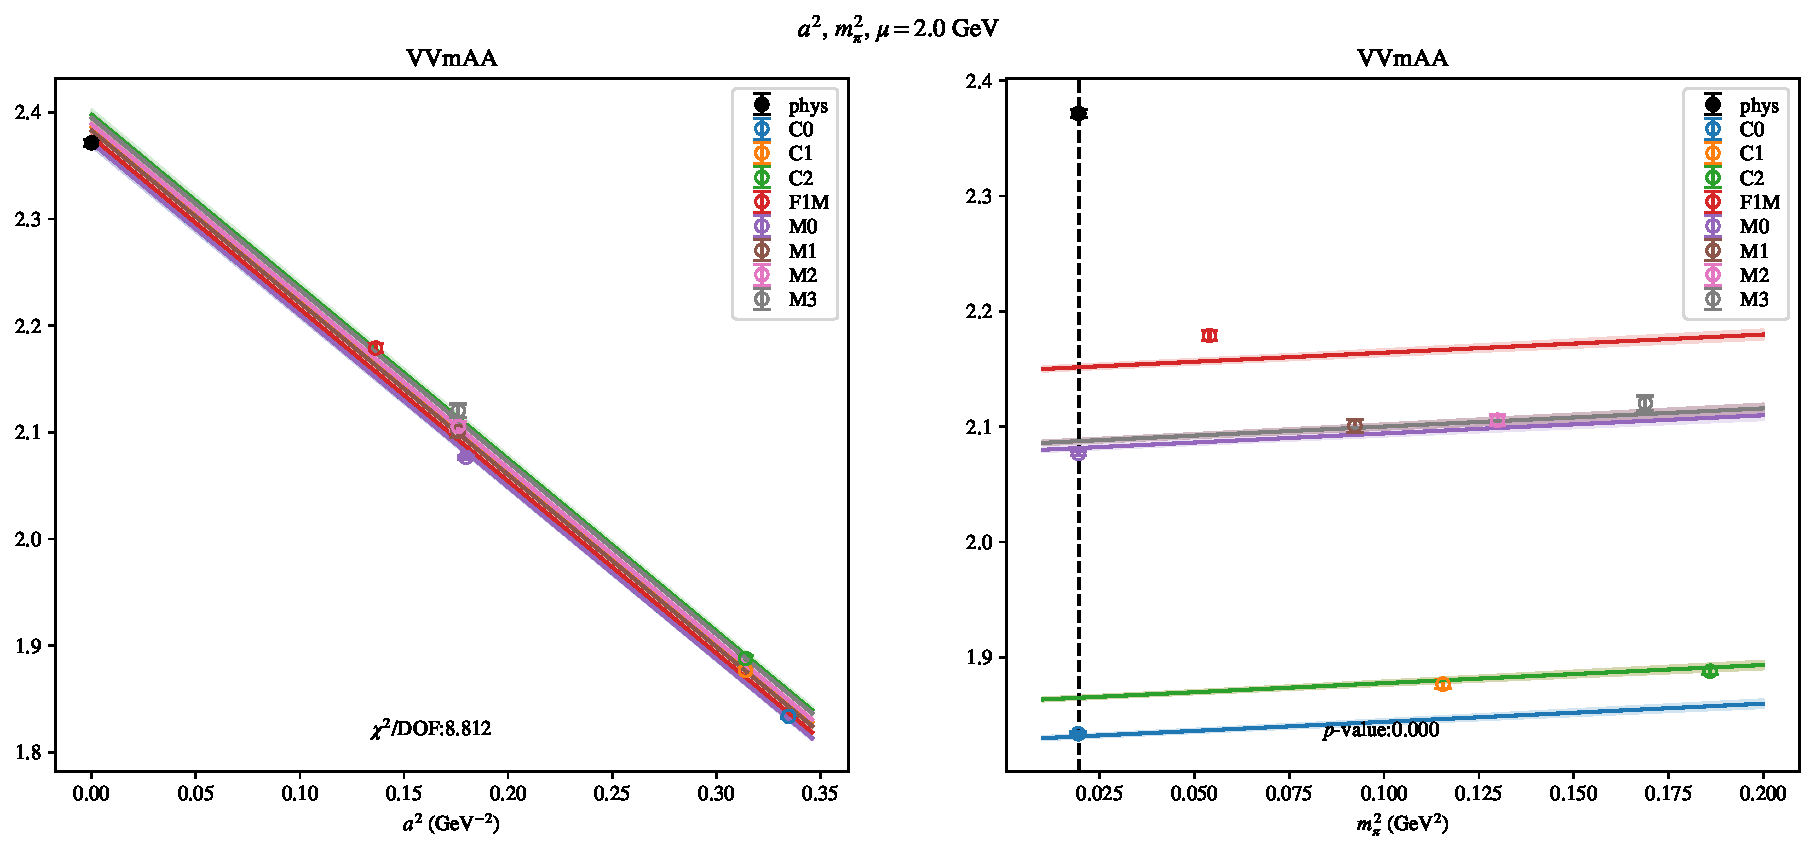
\includepdf[link, pages=-]{VVmAA/a2m2_20.pdf}
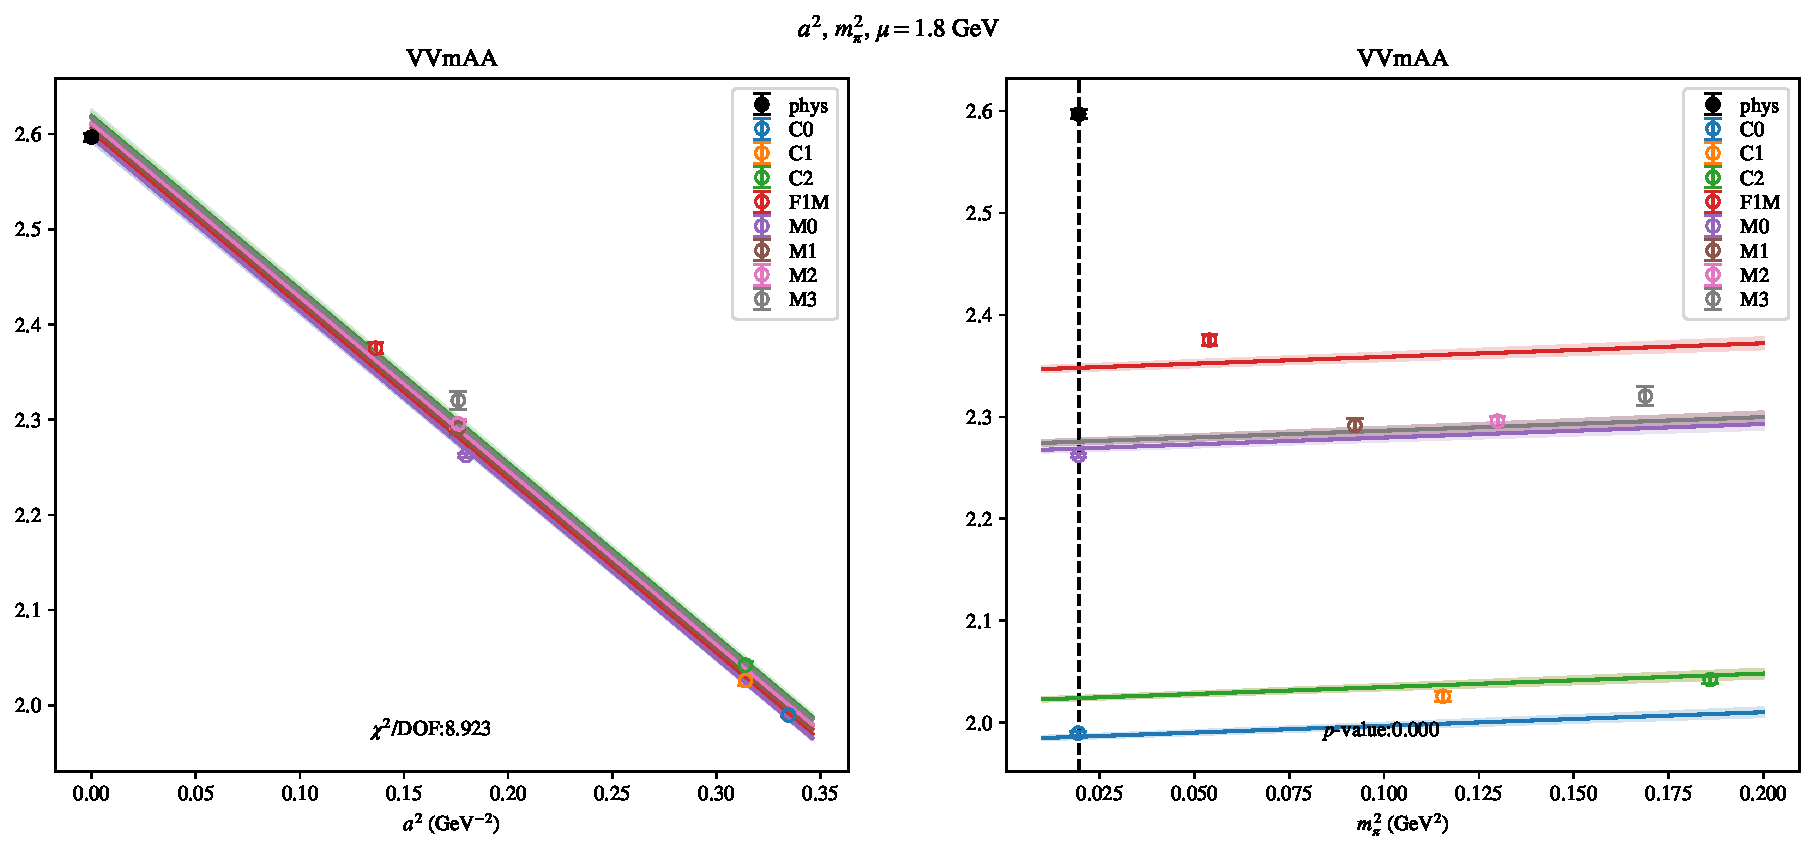
\includepdf[link, pages=-]{VVmAA/a2m2_18.pdf}
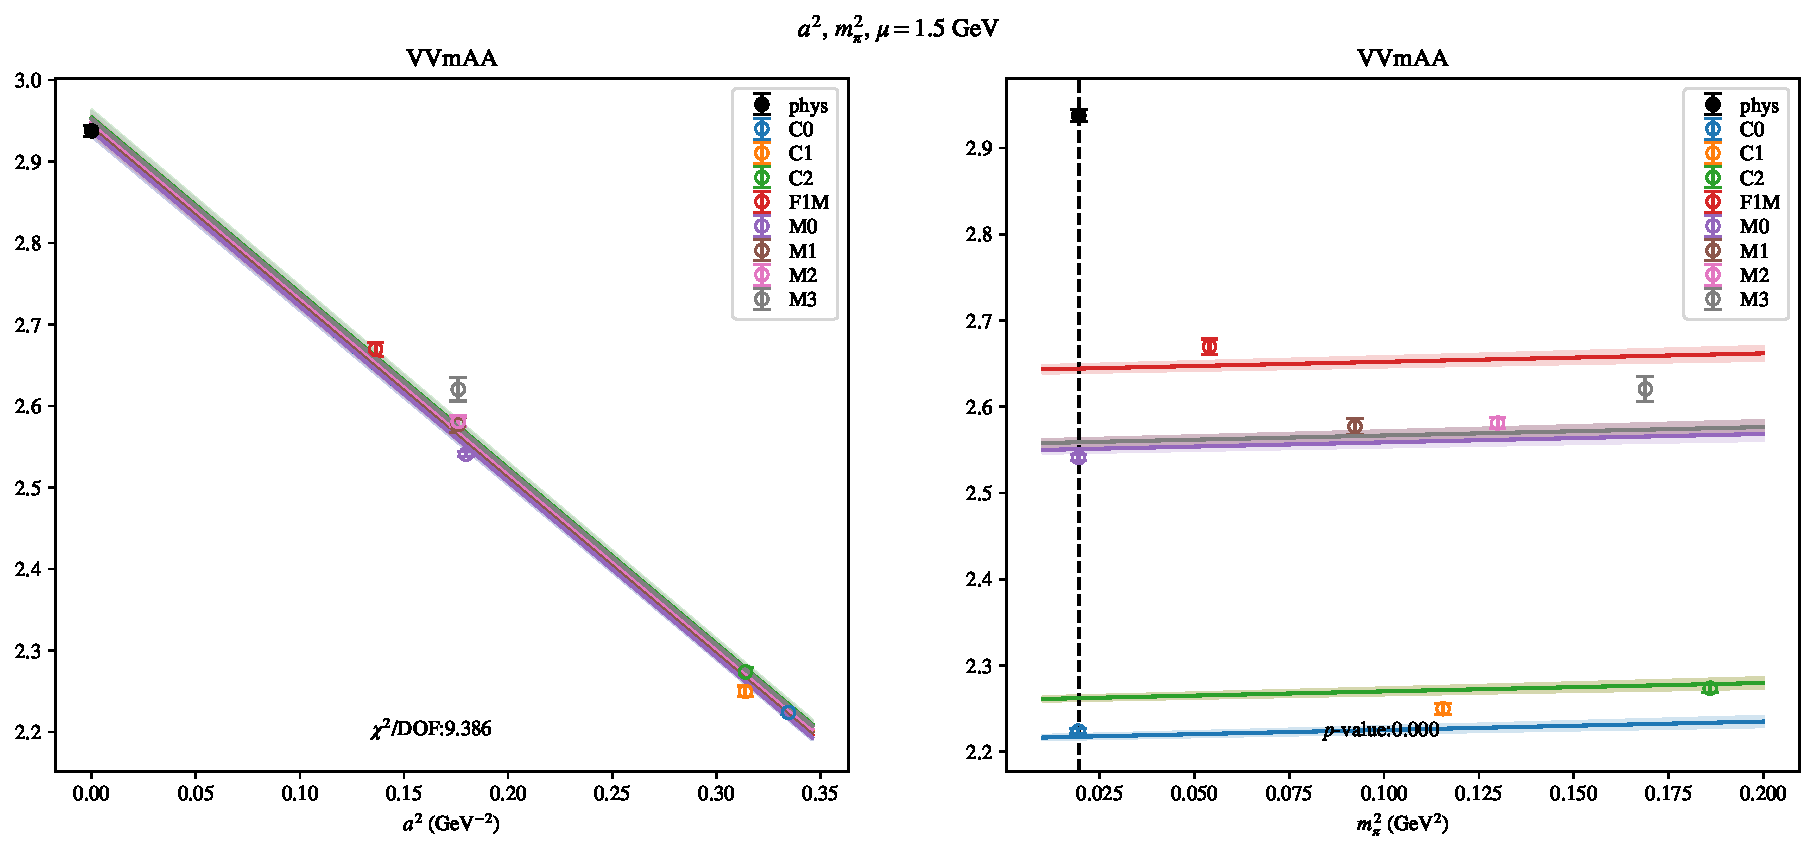
\includepdf[link, pages=-]{VVmAA/a2m2_15.pdf}
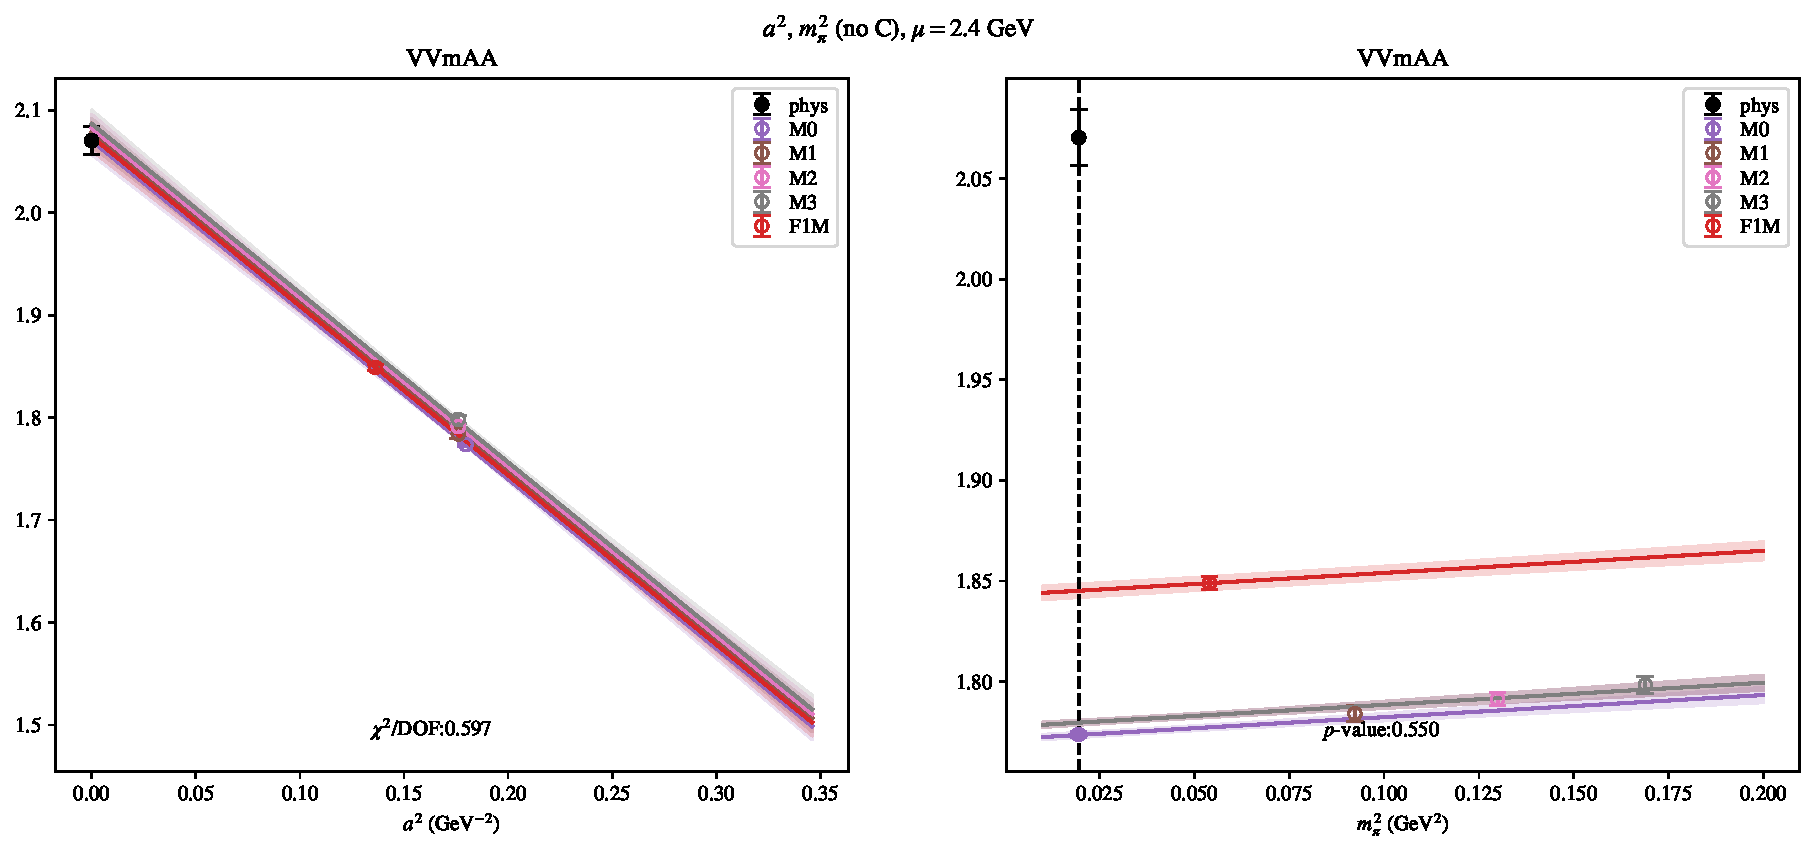
\includepdf[link, pages=-]{VVmAA/a2m2noC_24.pdf}
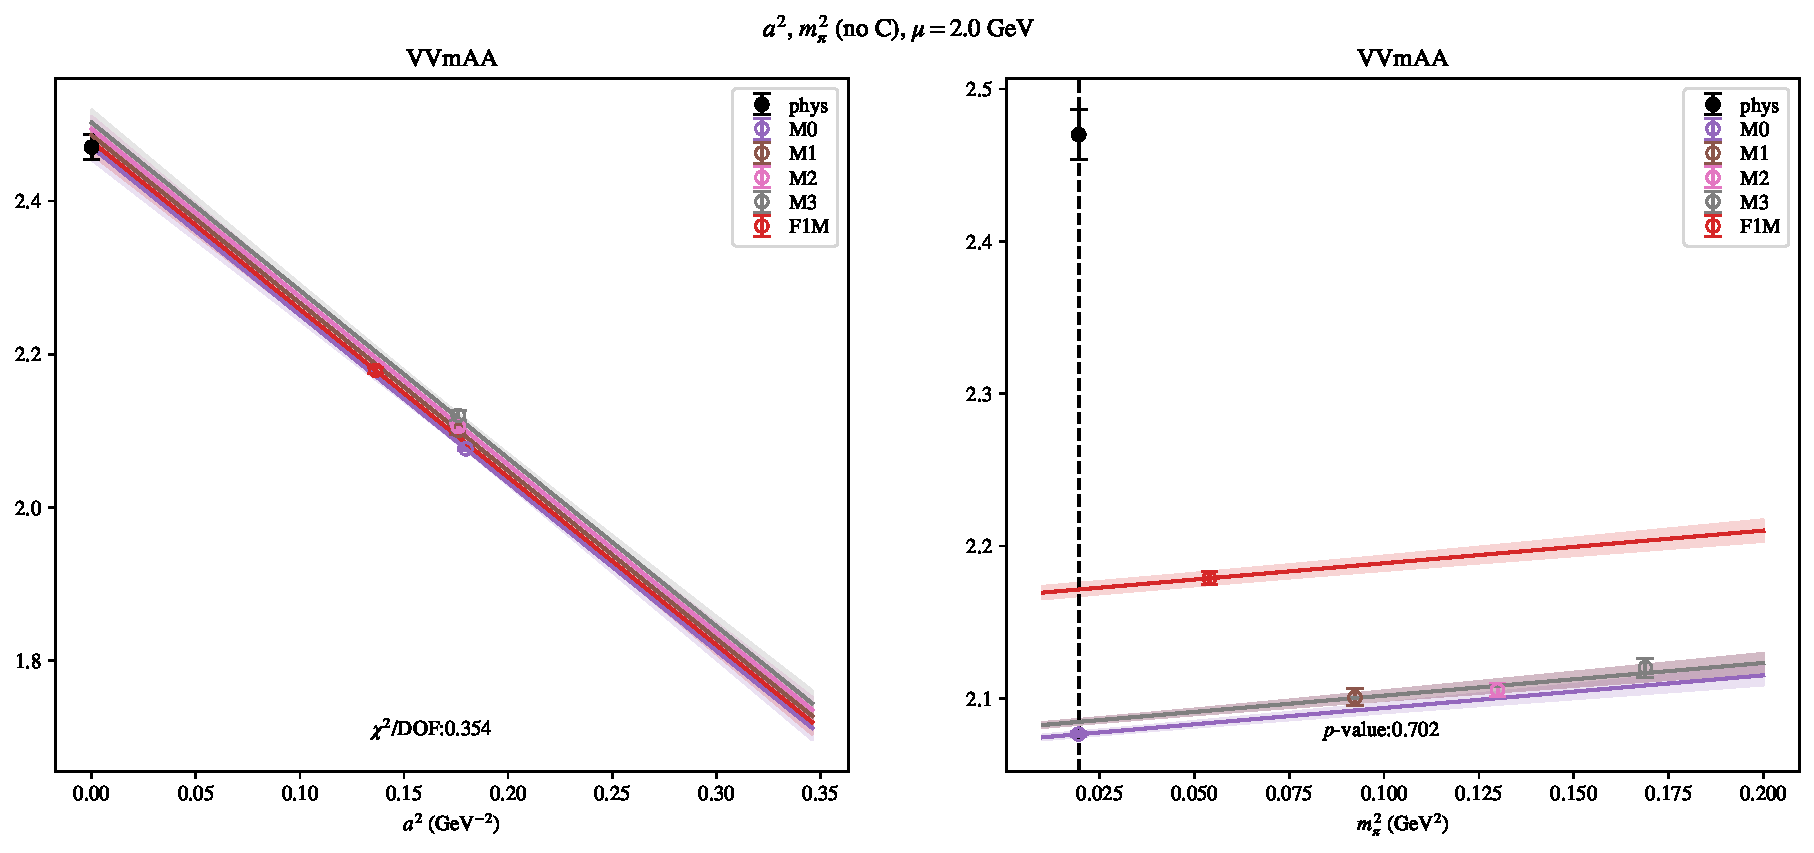
\includepdf[link, pages=-]{VVmAA/a2m2noC_20.pdf}
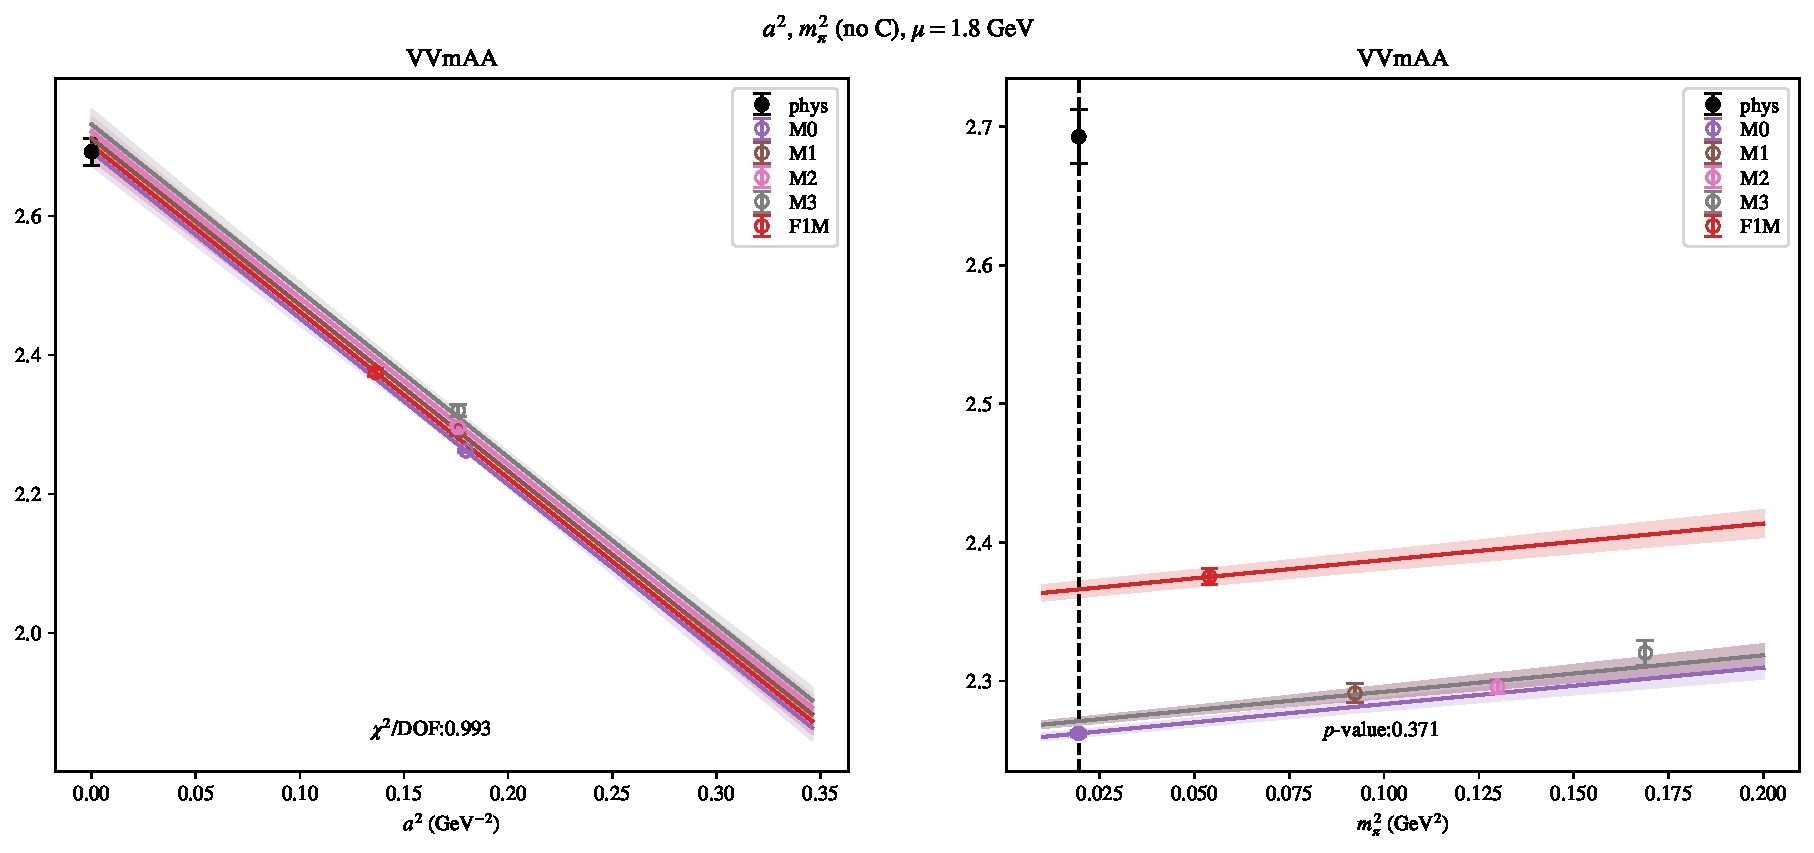
\includepdf[link, pages=-]{VVmAA/a2m2noC_18.pdf}
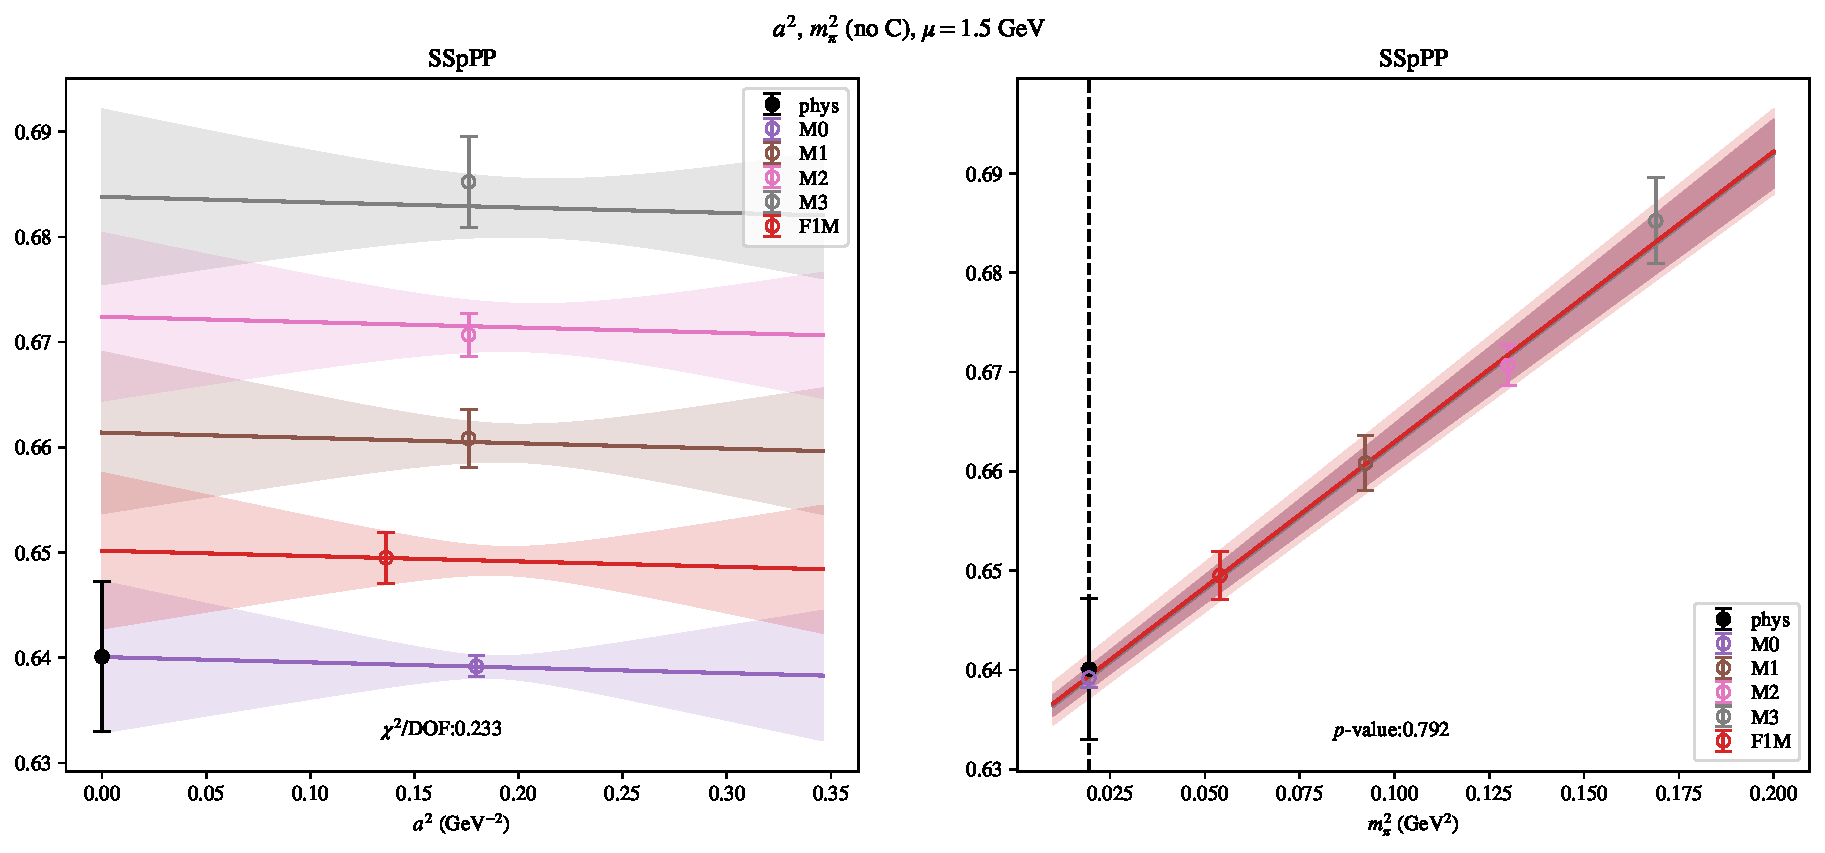
\includepdf[link, pages=-]{VVmAA/a2m2noC_15.pdf}
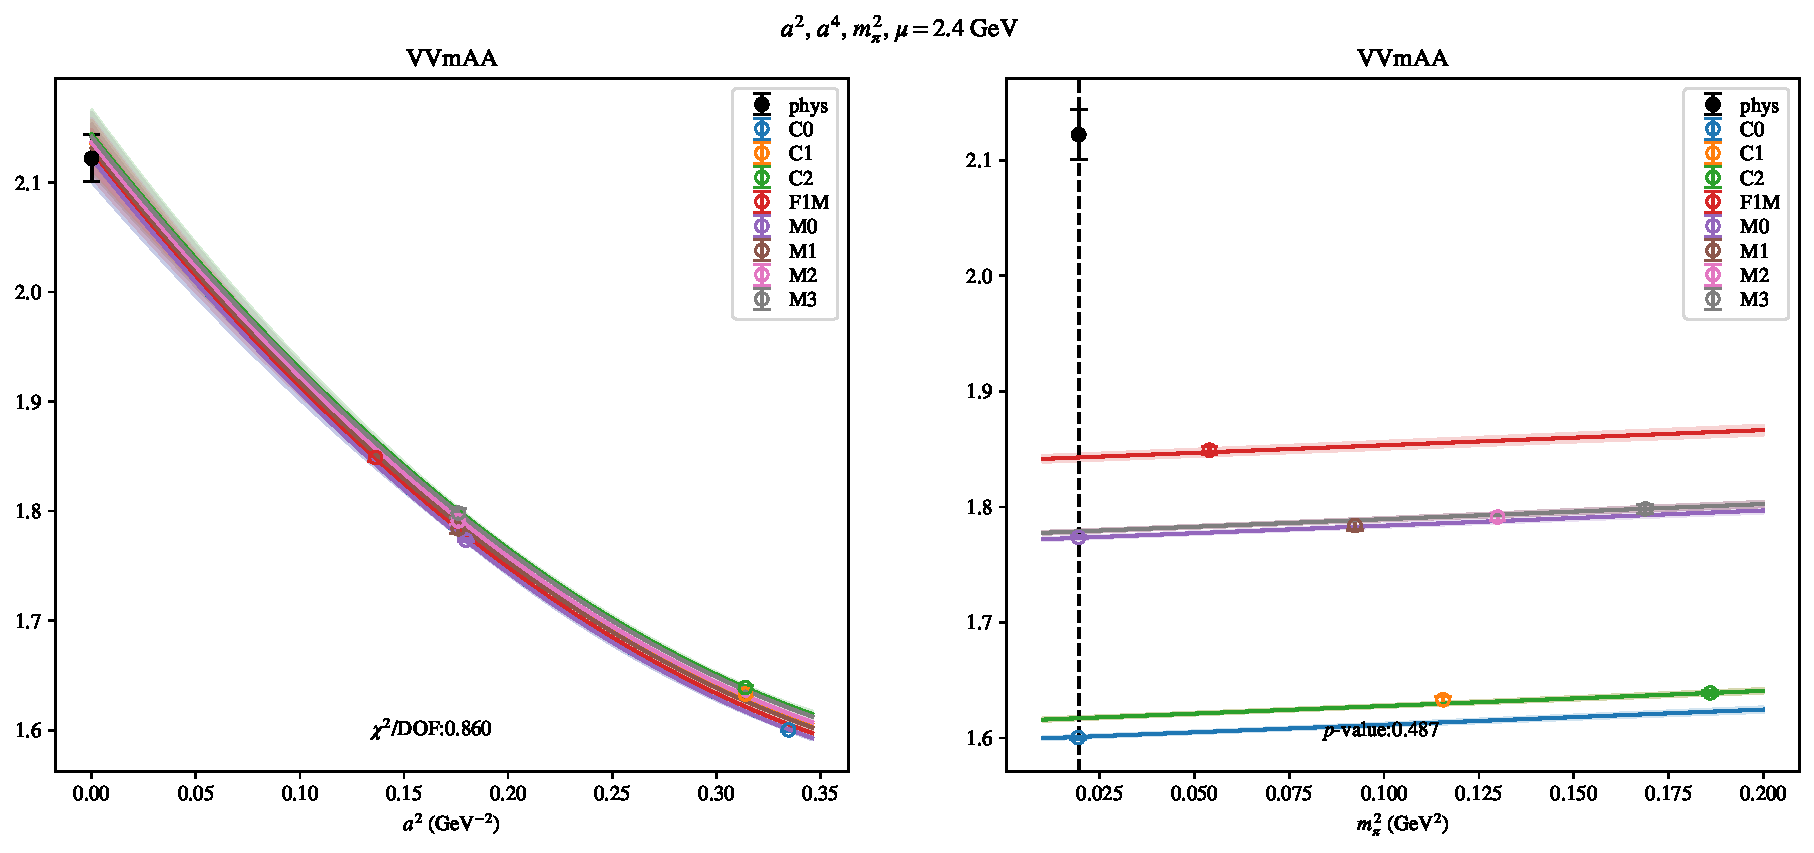
\includepdf[link, pages=-]{VVmAA/a2a4m2_24.pdf}
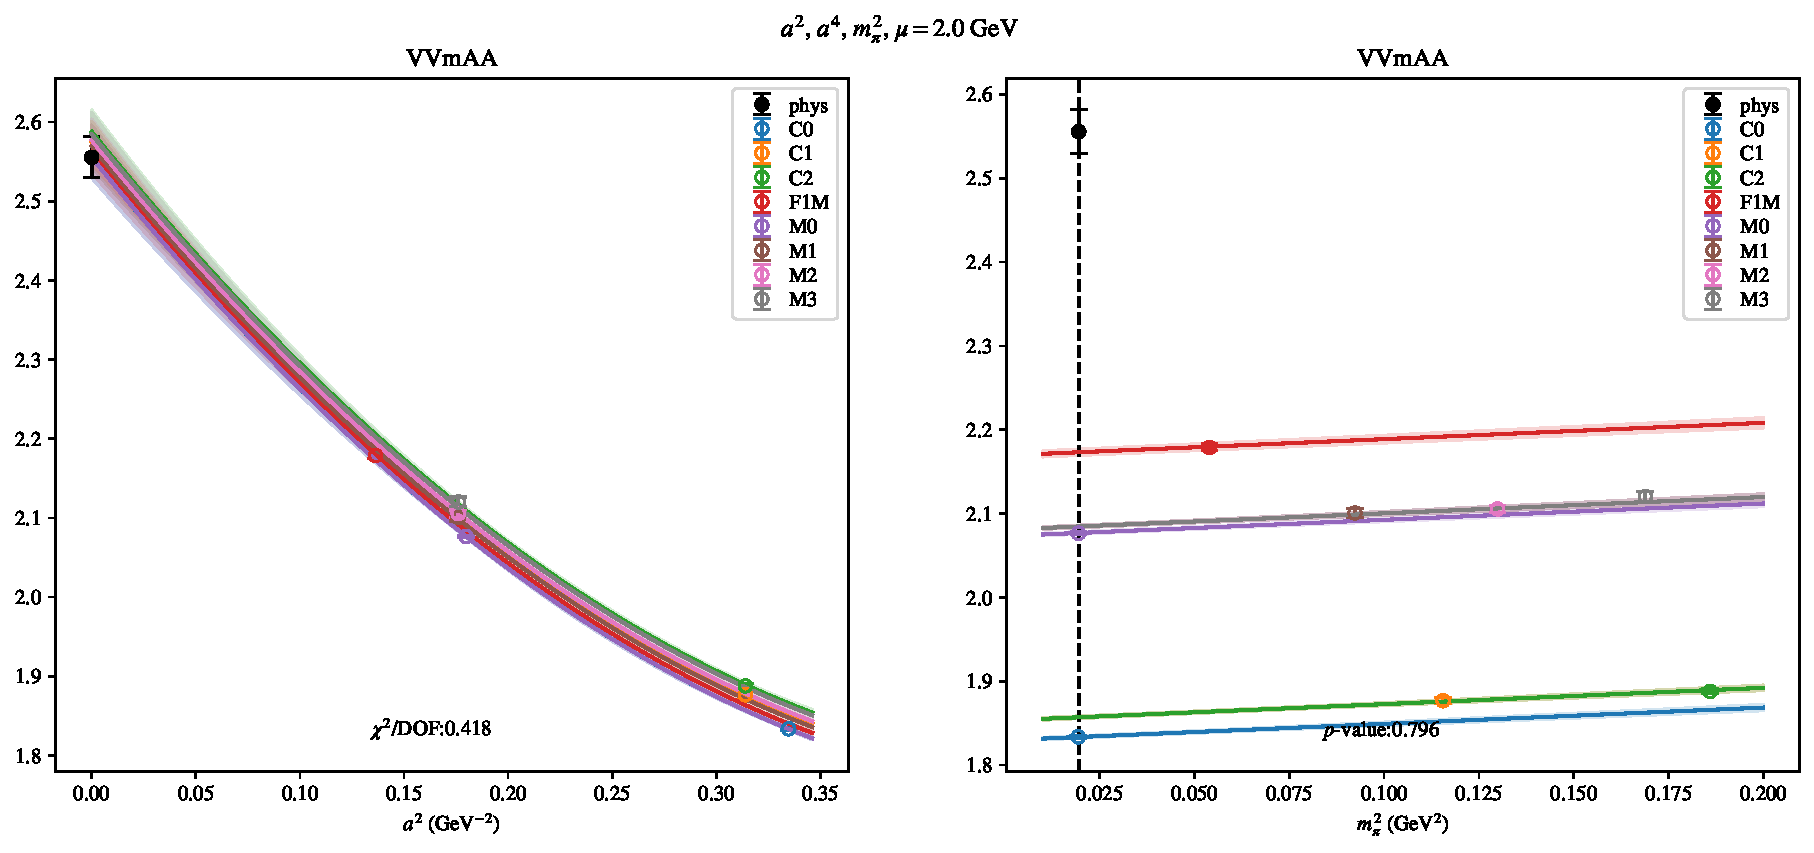
\includepdf[link, pages=-]{VVmAA/a2a4m2_20.pdf}
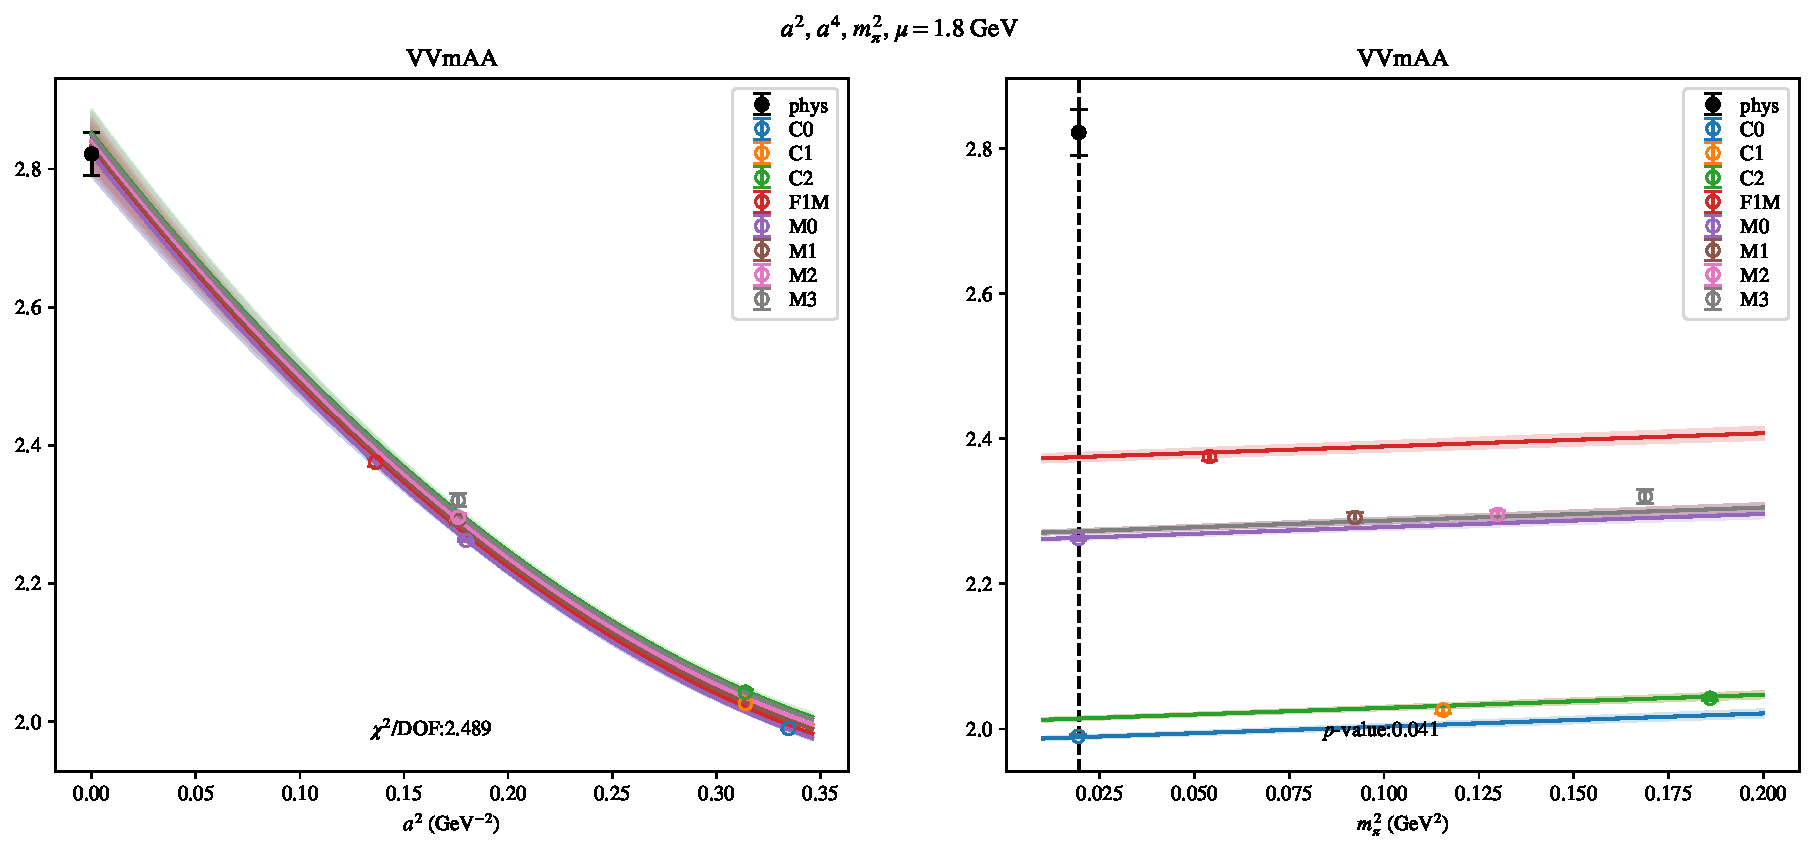
\includepdf[link, pages=-]{VVmAA/a2a4m2_18.pdf}
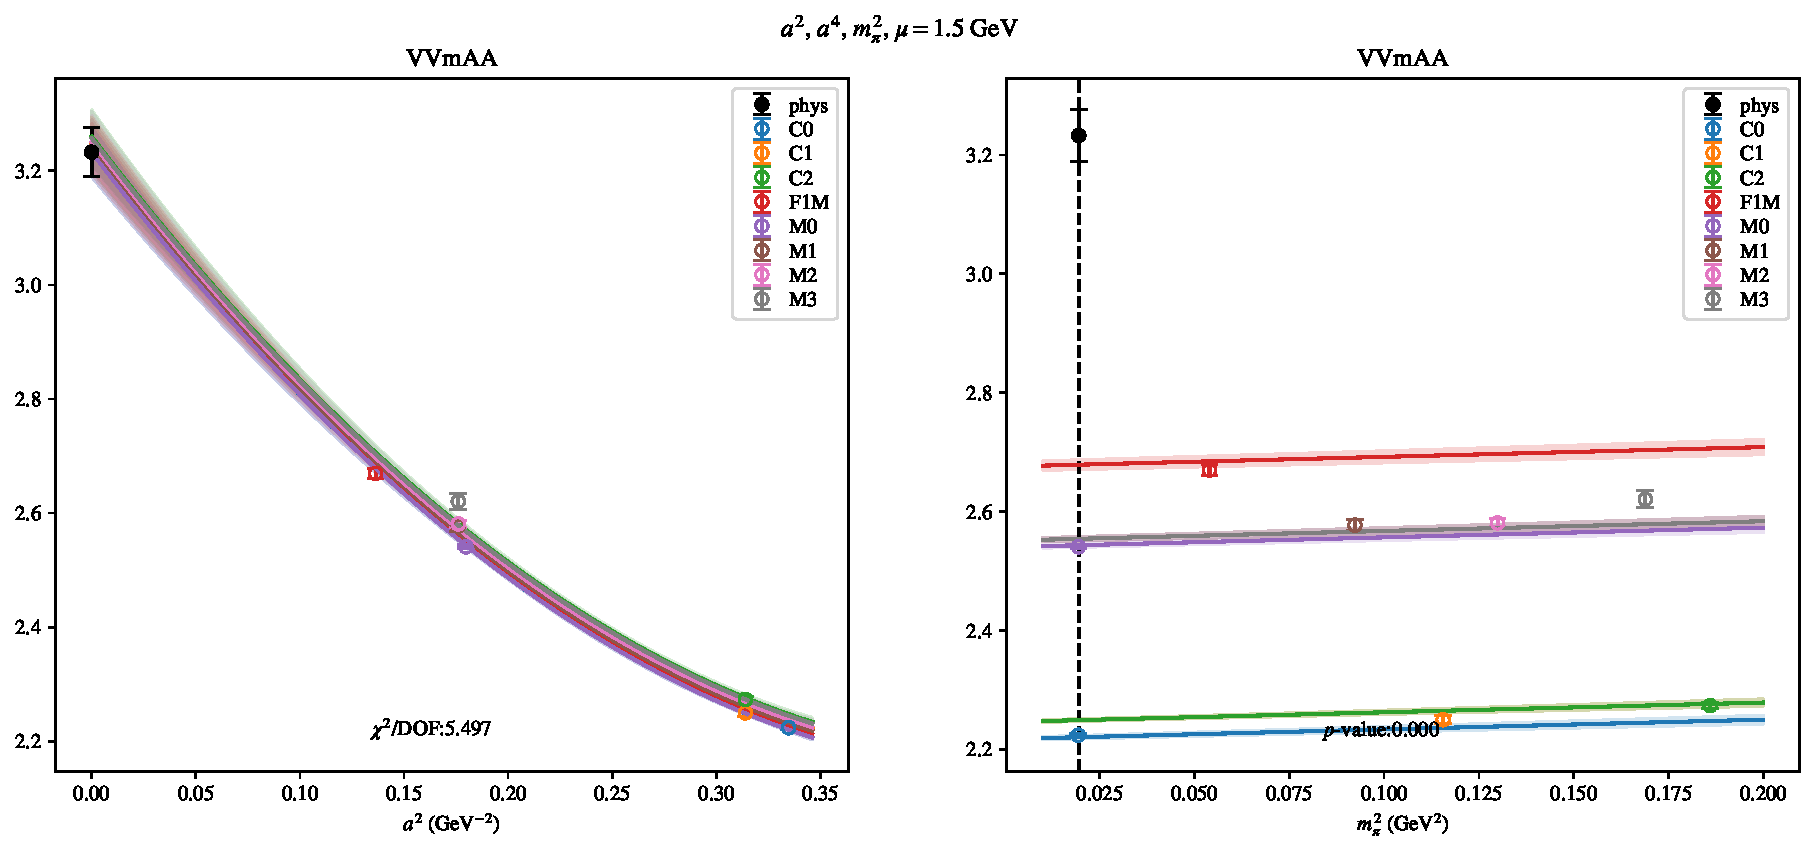
\includepdf[link, pages=-]{VVmAA/a2a4m2_15.pdf}
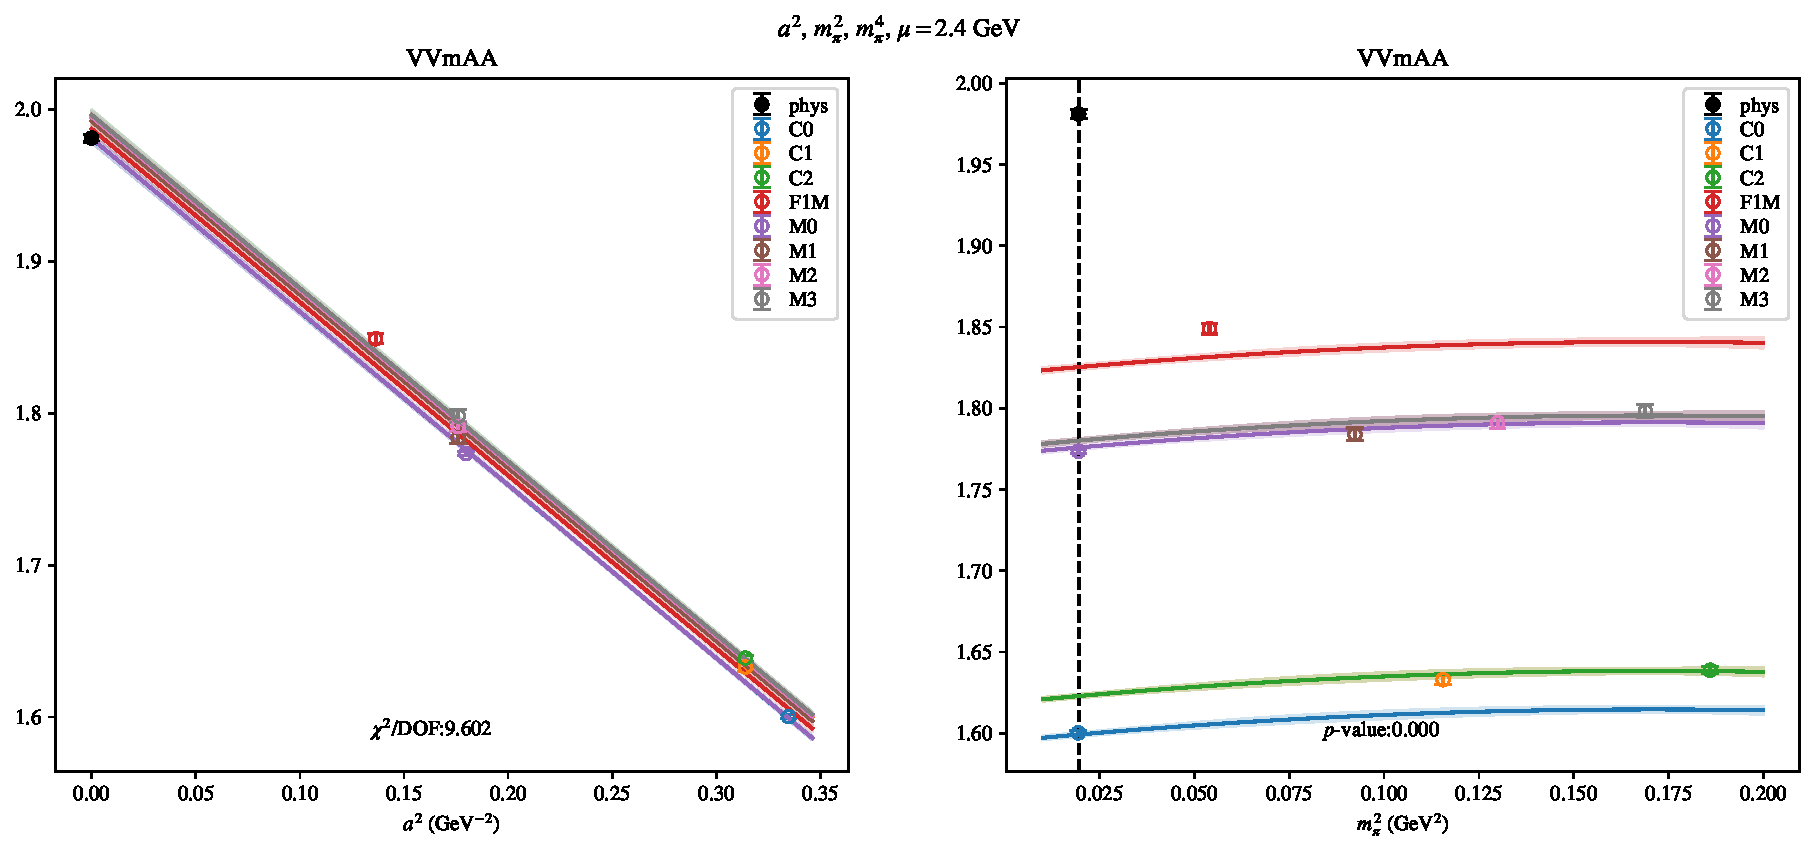
\includepdf[link, pages=-]{VVmAA/a2m2m4_24.pdf}
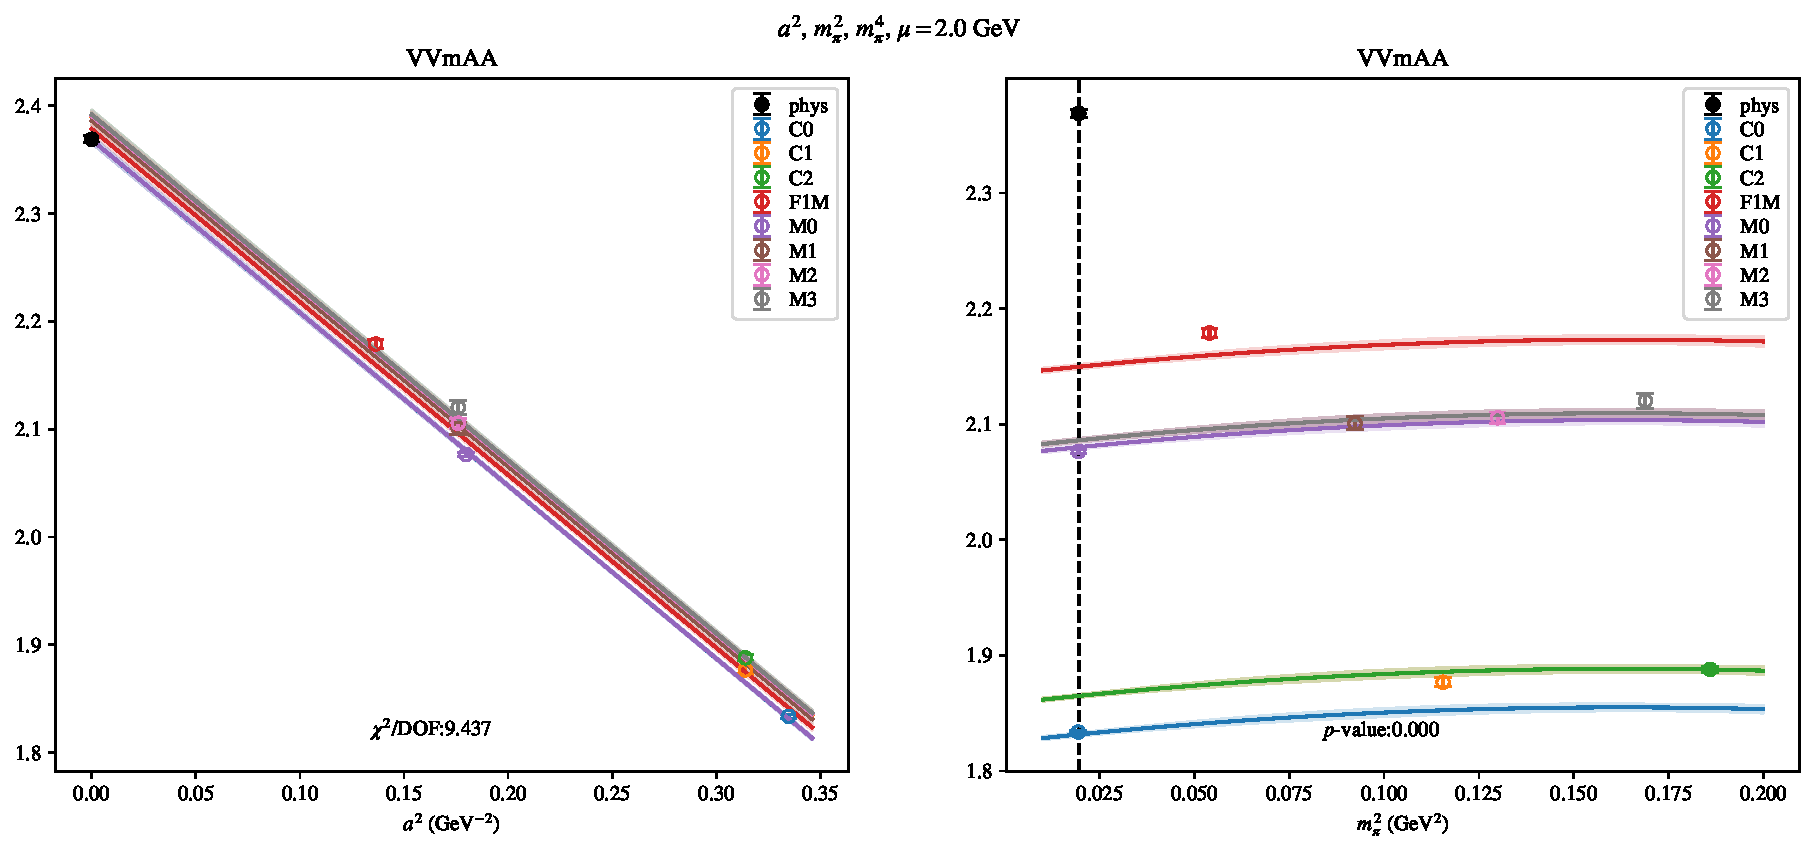
\includepdf[link, pages=-]{VVmAA/a2m2m4_20.pdf}
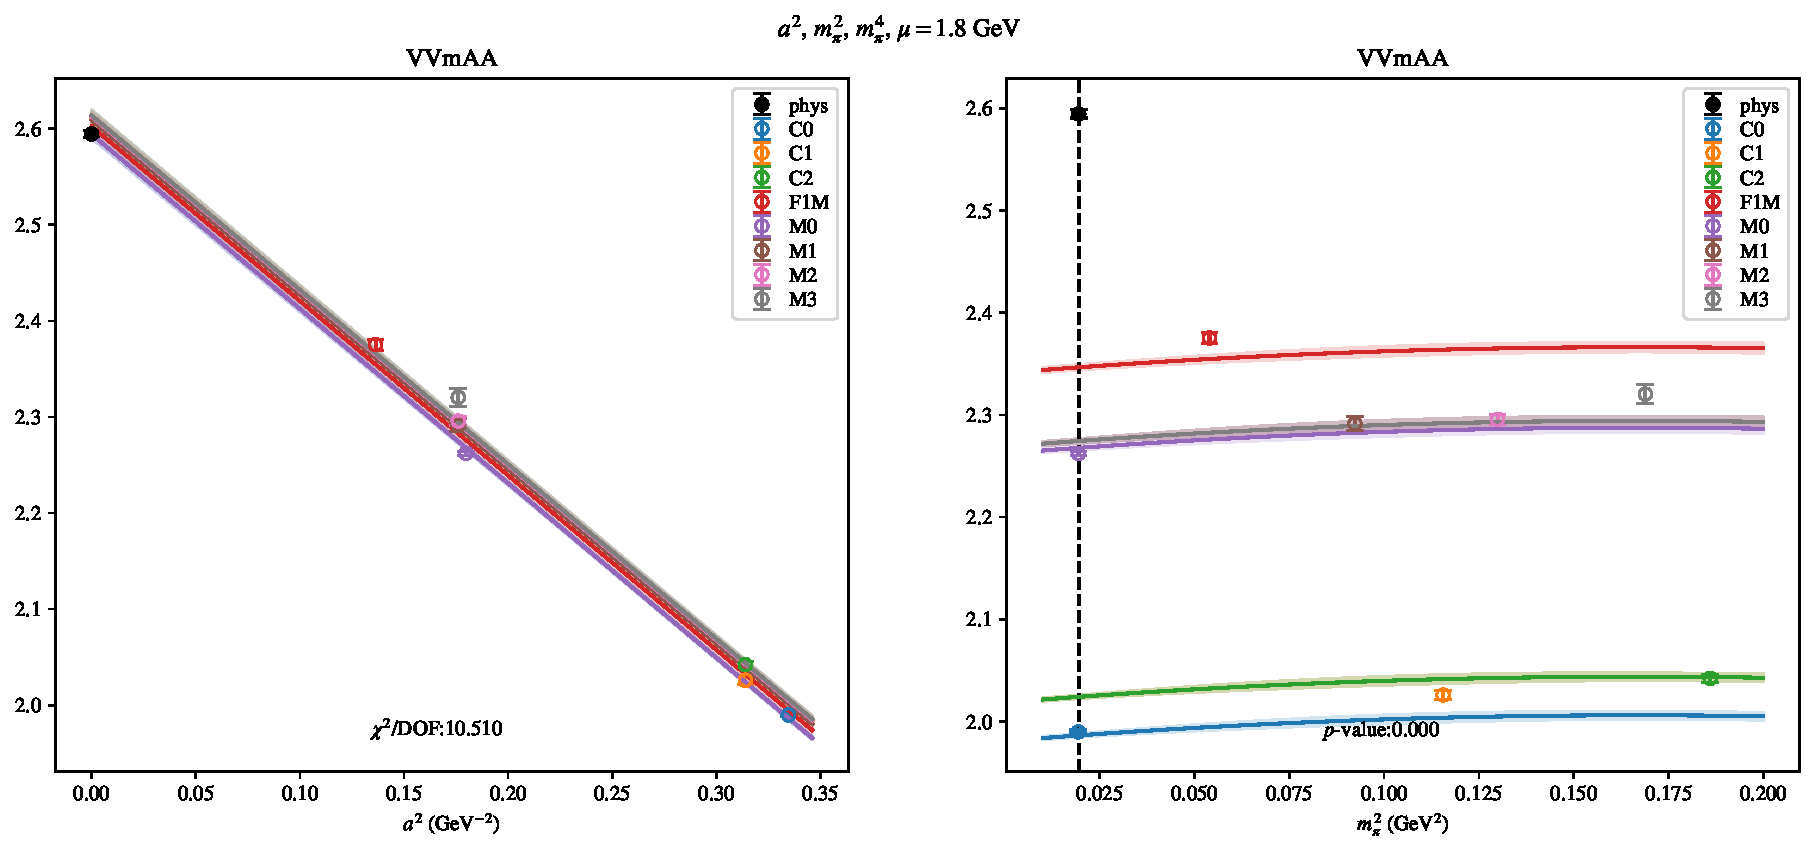
\includepdf[link, pages=-]{VVmAA/a2m2m4_18.pdf}
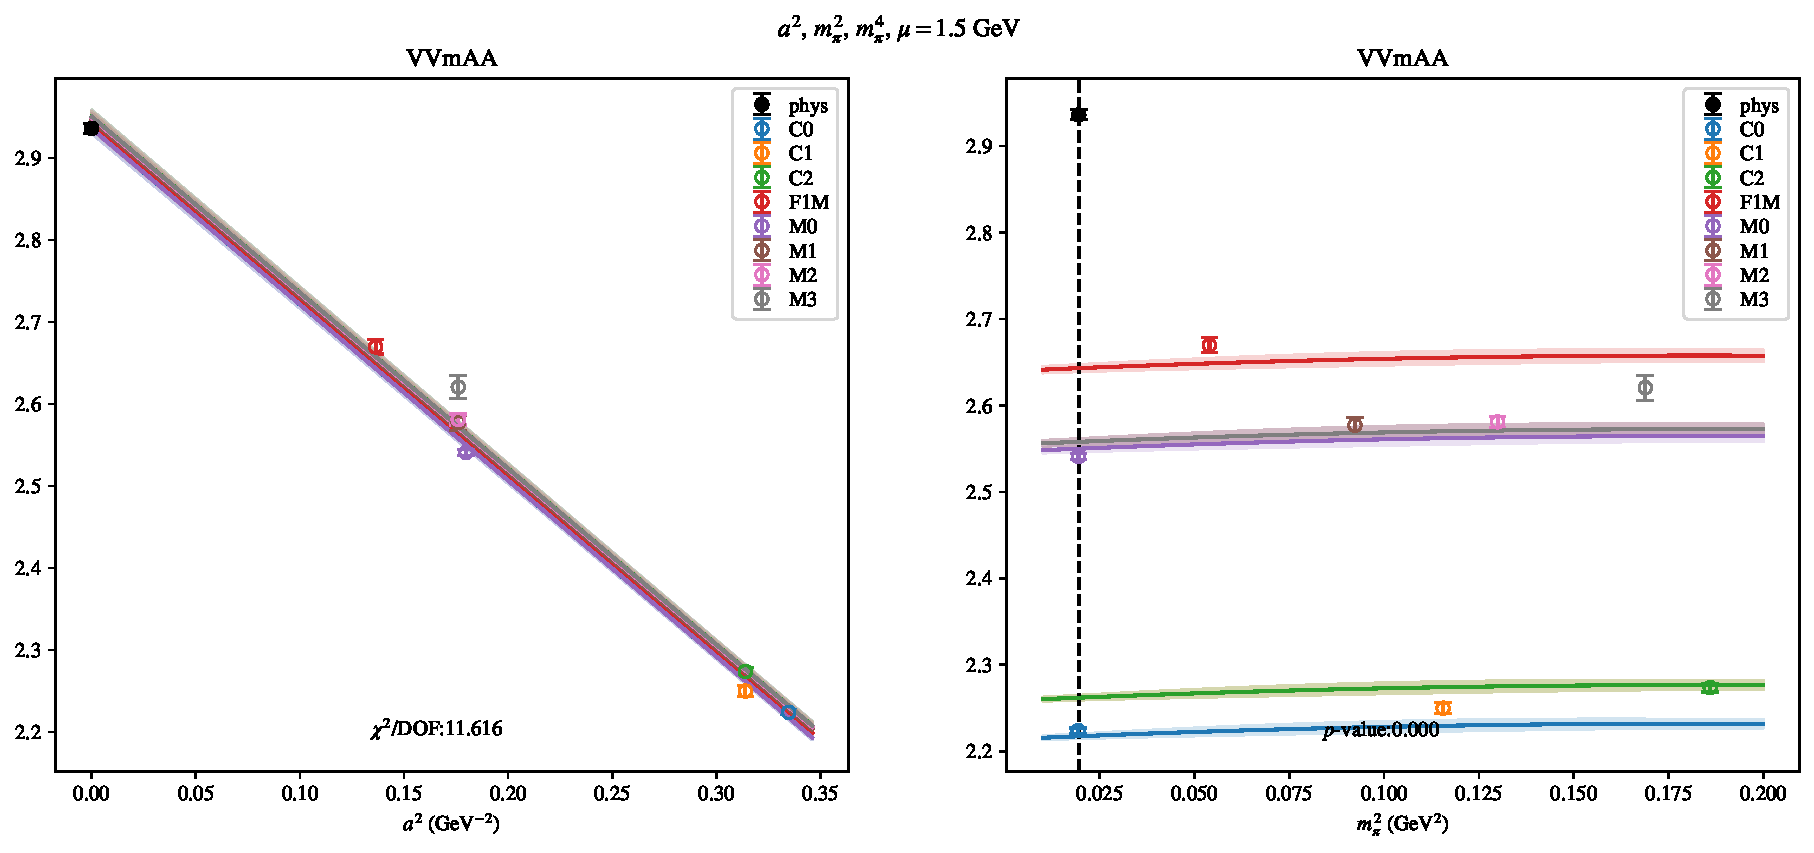
\includepdf[link, pages=-]{VVmAA/a2m2m4_15.pdf}
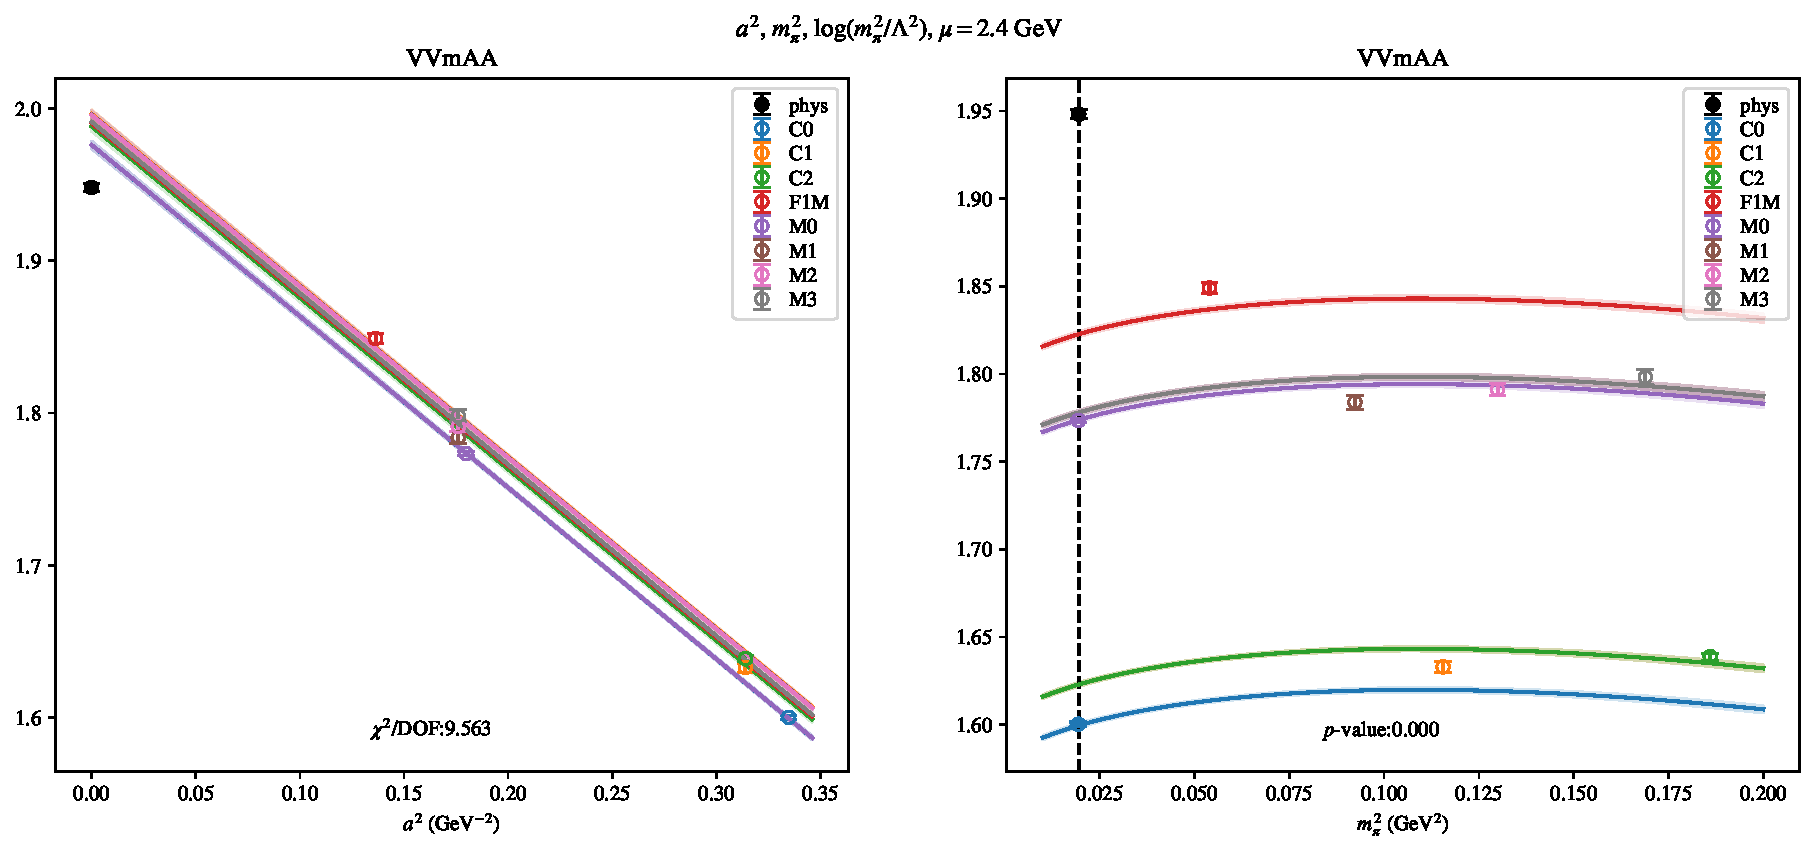
\includepdf[link, pages=-]{VVmAA/a2m2logm2_24.pdf}
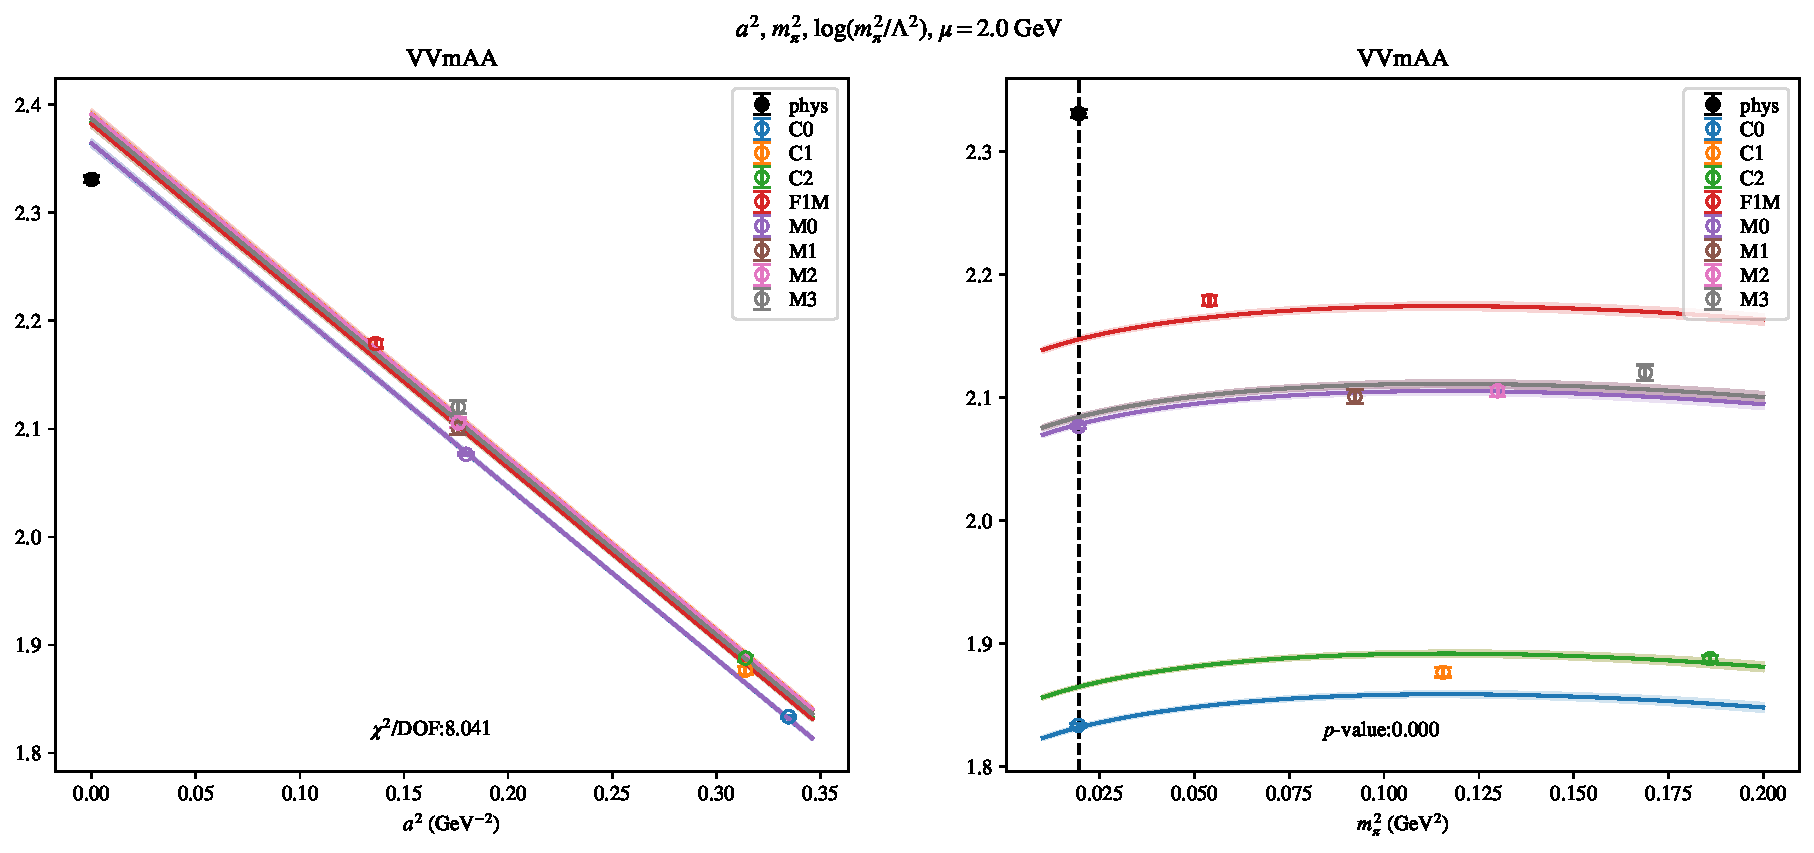
\includepdf[link, pages=-]{VVmAA/a2m2logm2_20.pdf}
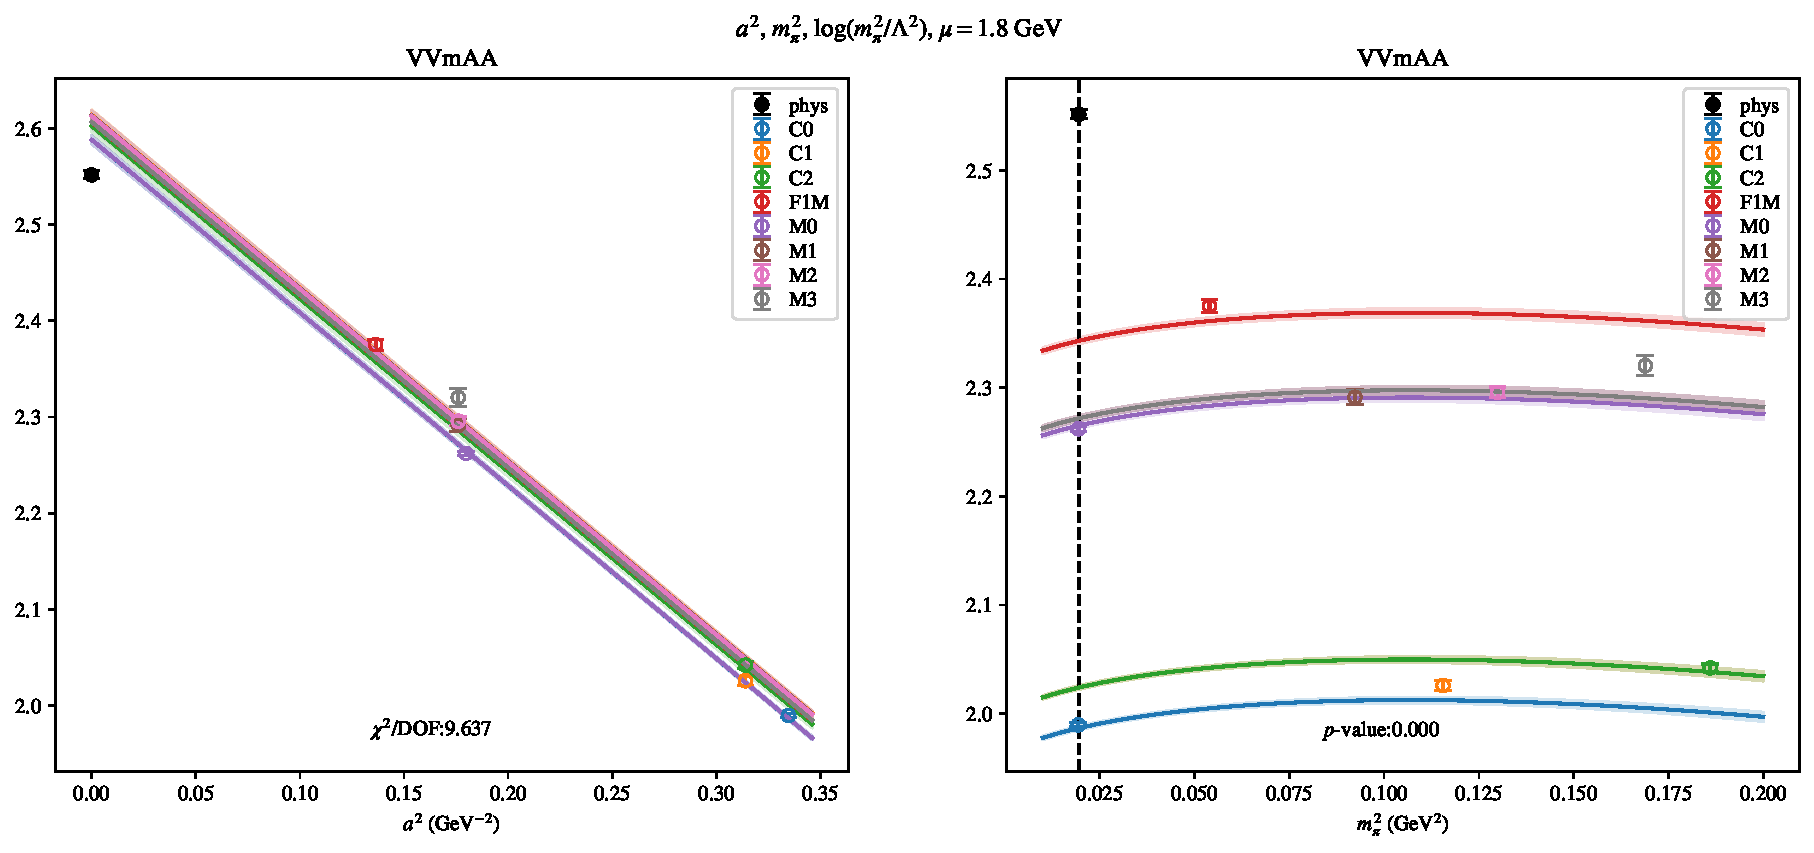
\includepdf[link, pages=-]{VVmAA/a2m2logm2_18.pdf}
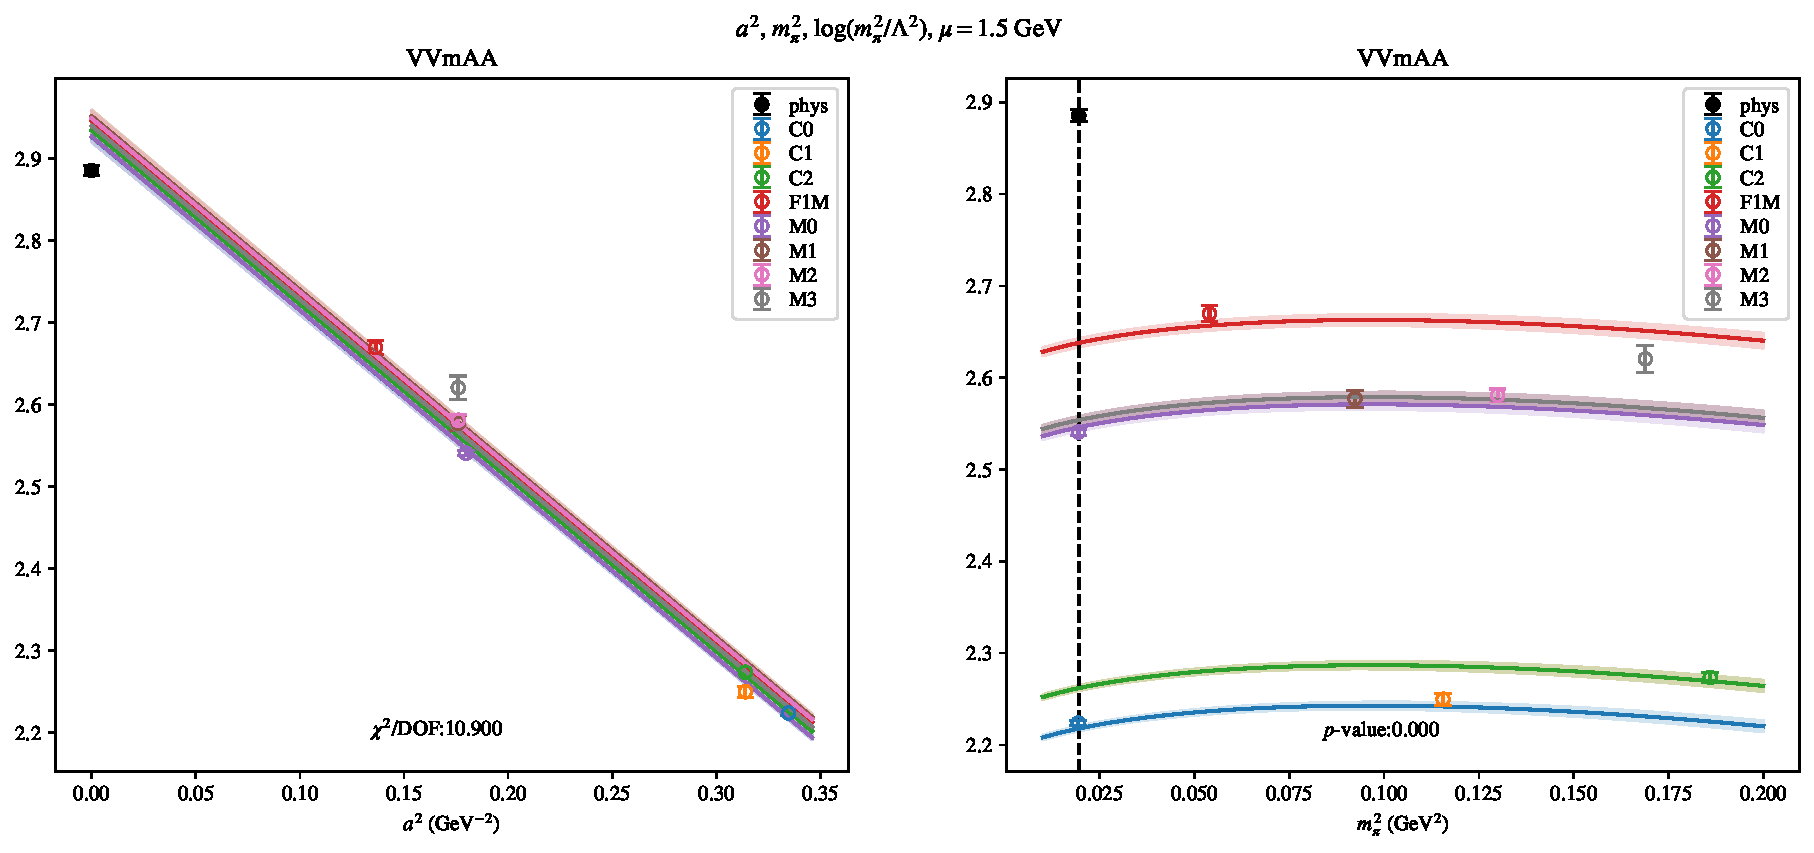
\includepdf[link, pages=-]{VVmAA/a2m2logm2_15.pdf}
\clearpage
\section{$B_3$}
\begin{table}[h!]
\begin{center}
\begin{tabular}{|c|c|c|c|c|c|}
\hline
$\mu$ (GeV) & $a^2$, $m_\pi^2$& $a^2$, $m_\pi^2$ (no C)& $a^2$, $a^4$, $m_\pi^2$& $a^2$, $m_\pi^2$, $m_\pi^4$& $a^2$, $m_\pi^2$, $\log(m_\pi^2/\Lambda^2)$\\
\hline
2.4& \hyperlink{SSmPP/a2m2_24.pdf.1}{\textbf{-0.0070(14)}: 26.004 (0.0)} & \hyperlink{SSmPP/a2m2noC_24.pdf.1}{\textbf{-0.0010(55)}: 0.351 (0.704)} & \hyperlink{SSmPP/a2a4m2_24.pdf.1}{\textbf{-0.00053(32)}: 13.485 (0.0)} & \hyperlink{SSmPP/a2m2m4_24.pdf.1}{\textbf{-0.0072(14)}: 30.014 (0.0)} & \hyperlink{SSmPP/a2m2logm2_24.pdf.1}{\textbf{-0.0069(14)}: 26.521 (0.0)}\\
2.0& \hyperlink{SSmPP/a2m2_20.pdf.1}{\textbf{3.466809(35)}: 694.143 (0.0)} & \hyperlink{SSmPP/a2m2noC_20.pdf.1}{\textbf{0.000278(77)}: 95.283 (0.0)} & \hyperlink{SSmPP/a2a4m2_20.pdf.1}{\textbf{-0.00025(37)}: 49.221 (0.0)} & \hyperlink{SSmPP/a2m2m4_20.pdf.1}{\textbf{0.00400(13)}: 503.364 (0.0)} & \hyperlink{SSmPP/a2m2logm2_20.pdf.1}{\textbf{3.480962(35)}: 694.135 (0.0)}\\
1.8& \hyperlink{SSmPP/a2m2_18.pdf.1}{\textbf{0.000319(44)}: 812.613 (0.0)} & \hyperlink{SSmPP/a2m2noC_18.pdf.1}{\textbf{0.000396(87)}: 69.934 (0.0)} & \hyperlink{SSmPP/a2a4m2_18.pdf.1}{\textbf{-0.00028(37)}: 33.553 (0.0)} & \hyperlink{SSmPP/a2m2m4_18.pdf.1}{\textbf{0.00659(20)}: 599.073 (0.0)} & \hyperlink{SSmPP/a2m2logm2_18.pdf.1}{\textbf{0.000319(44)}: 812.613 (0.0)}\\
1.5& \hyperlink{SSmPP/a2m2_15.pdf.1}{\textbf{0.000524(51)}: 764.646 (0.0)} & \hyperlink{SSmPP/a2m2noC_15.pdf.1}{\textbf{0.0525(30)}: 0.345 (0.708)} & \hyperlink{SSmPP/a2a4m2_15.pdf.1}{\textbf{-0.00031(39)}: 23.553 (0.0)} & \hyperlink{SSmPP/a2m2m4_15.pdf.1}{\textbf{0.01037(32)}: 550.908 (0.0)} & \hyperlink{SSmPP/a2m2logm2_15.pdf.1}{\textbf{0.000524(51)}: 764.646 (0.0)}\\
\hline
\end{tabular}
\caption{Physical point value from chiral and continuum extrapolation at renormalisation scale $\mu$. Entries are \textbf{value(error)}: $\chi^2/\text{DOF}$ ($p$-value).}
\end{center}
\end{table}
\begin{table}[h!]
\begin{center}
\begin{tabular}{|c c|c|c|c|c|c|}
\hline
$\mu$ (GeV) &  & $a^2$, $m_\pi^2$& $a^2$, $m_\pi^2$ (no C)& $a^2$, $a^4$, $m_\pi^2$& $a^2$, $m_\pi^2$, $m_\pi^4$& $a^2$, $m_\pi^2$, $\log(m_\pi^2/\Lambda^2)$\\
\hline
\multirow{2}{0.5in}{2.4} & $\alpha$ & 26.1(61)& 2(19)& 93(79)& 24.6(63)& 26.4(62)\\
 & $\beta$ & 0.0394(22)& 0.17(12)& 0.983(87)& 0.007& 0.0351(22)\\
\hline
\multirow{2}{0.5in}{2.0} & $\alpha$ & 3(87)& 5(46)& 10(92)& 4(47)& 3(92)\\
 & $\beta$ & -7.(75)& -13(41)& 2.67(38)& -1(38)& -8.(75)\\
\hline
\multirow{2}{0.5in}{1.8} & $\alpha$ & (14)& (38)& -1(83)& 9(78)& (11)\\
 & $\beta$ & -1(27)& -1(74)& 5.53(76)& -(16)& -1(27)\\
\hline
\multirow{2}{0.5in}{1.5} & $\alpha$ & 268390.76444720(10)& -4.55(34)& (13)& (88)& 270037.3163942583(10)\\
 & $\beta$ & -(49)& 0.0050(14)& 27.(28)& (24)& -(49)\\
\hline
\end{tabular}
\caption{Fit values of coefficients in $B = B_0(1 + \mathbf{\alpha} a^2 + \mathbf{\beta} \frac{m_\pi^2}{f_\pi^2} + \ldots)$.}
\end{center}
\end{table}
\begin{figure}
\centering
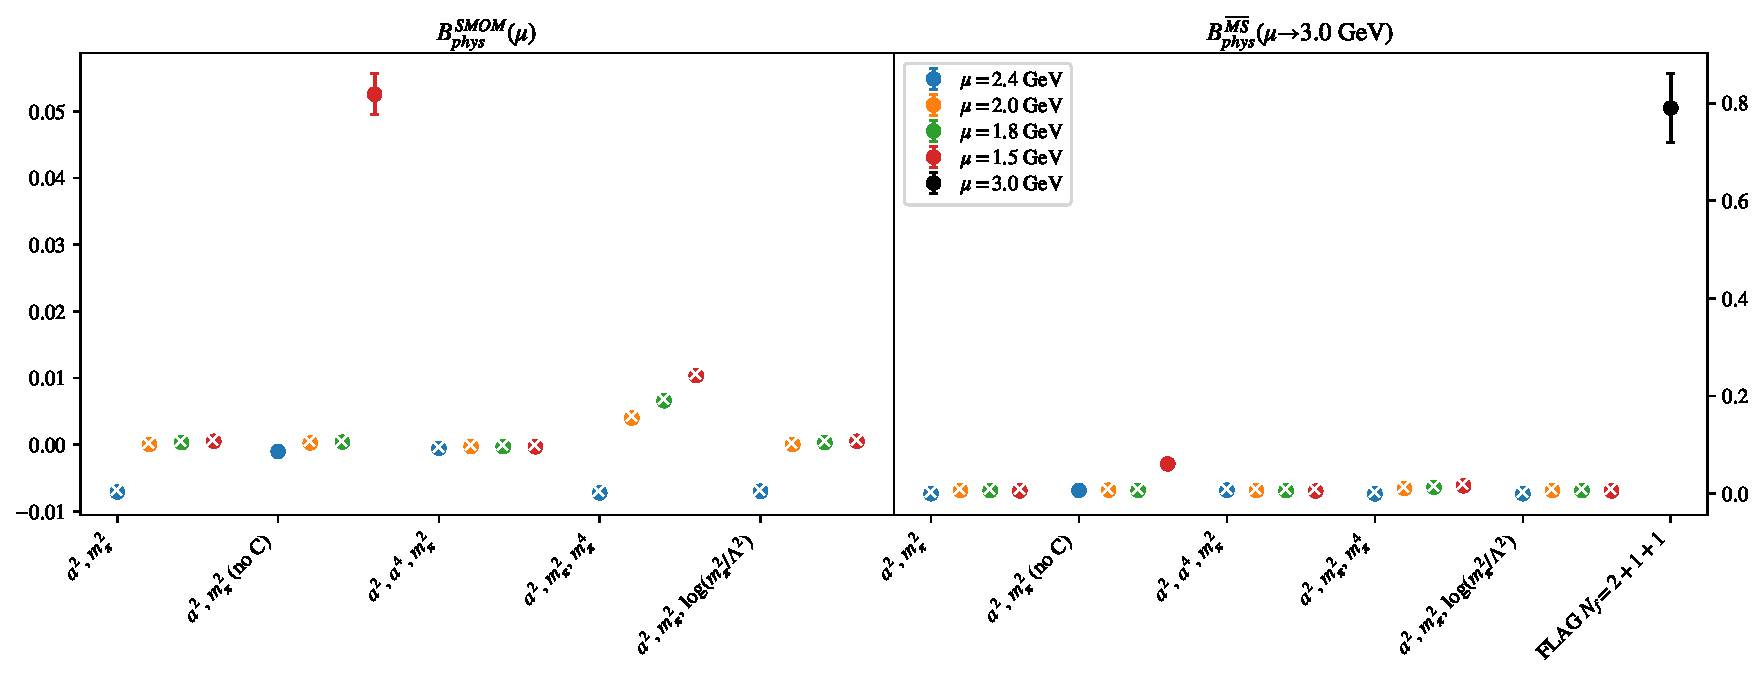
\includegraphics[page=1, width=1.1\textwidth]{plots/SSmPP_fit_summary.pdf}
\caption{\\(left) $B_{phys}$ in RI/SMOM scheme from fit variations (fits with $p$-value $<0.05$ marked with ``$\times$"). \\(right) $B_{phys}$ in $\overline{MS}$ computed using $B^{\overline{MS}} = R^{\overline{MS}\leftarrow SMOM}(3.0)\sigma_{npt}^{F1M}(3.0, 2.0) B^{SMOM}$.}
\end{figure}
\clearpage
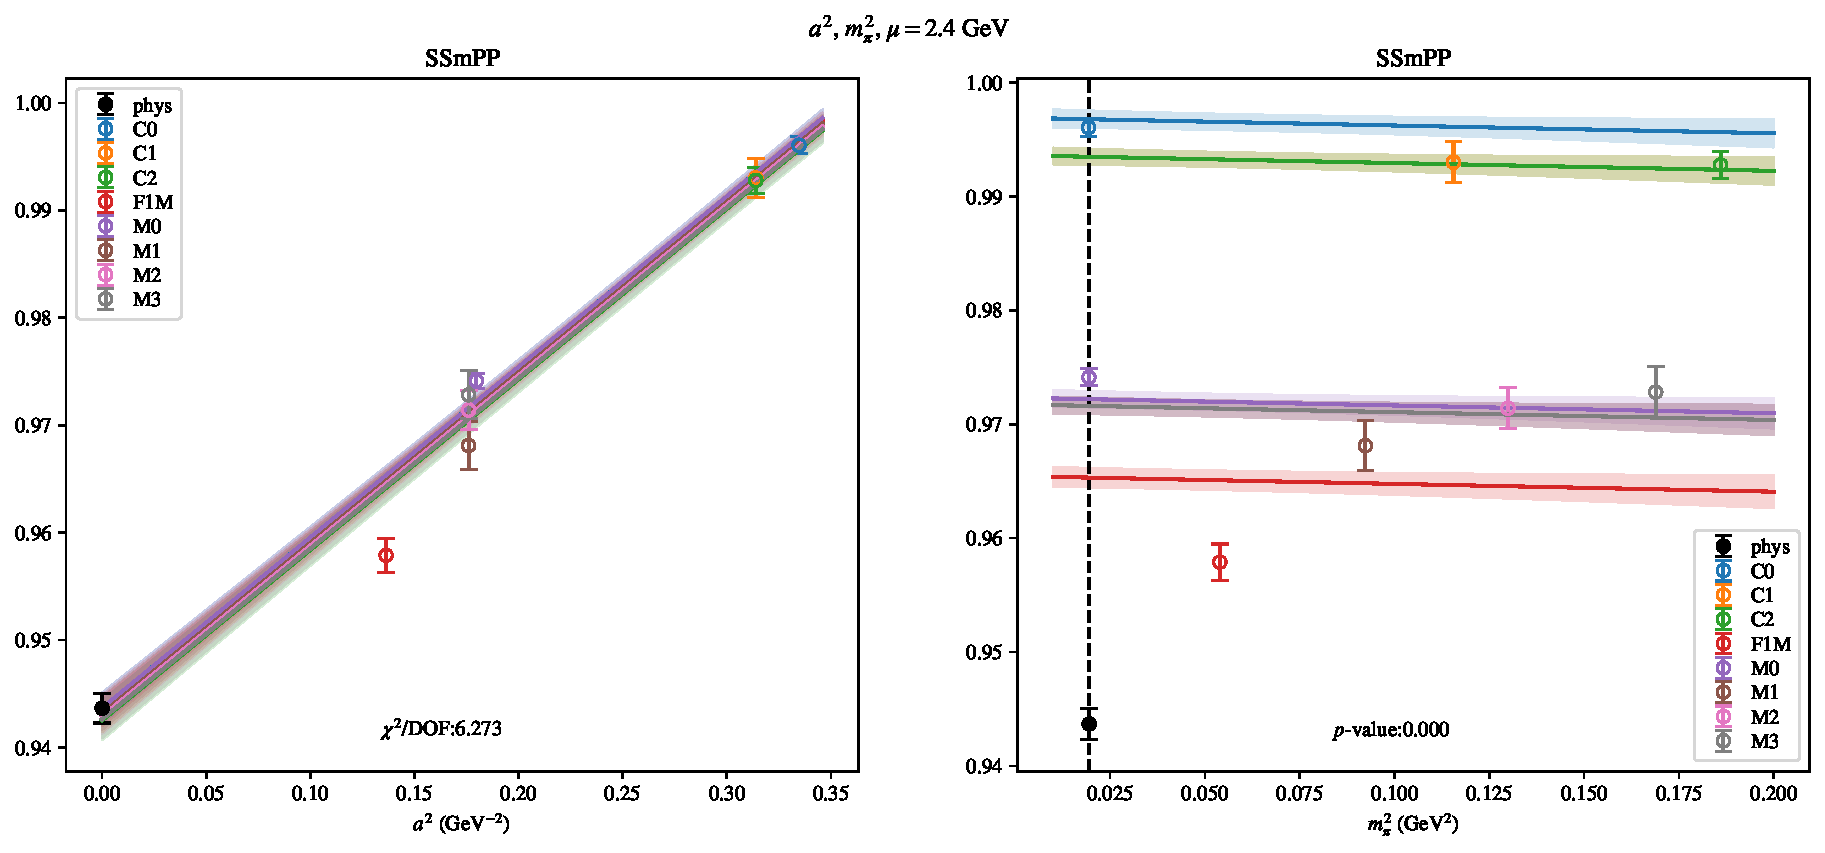
\includepdf[link, pages=-]{SSmPP/a2m2_24.pdf}
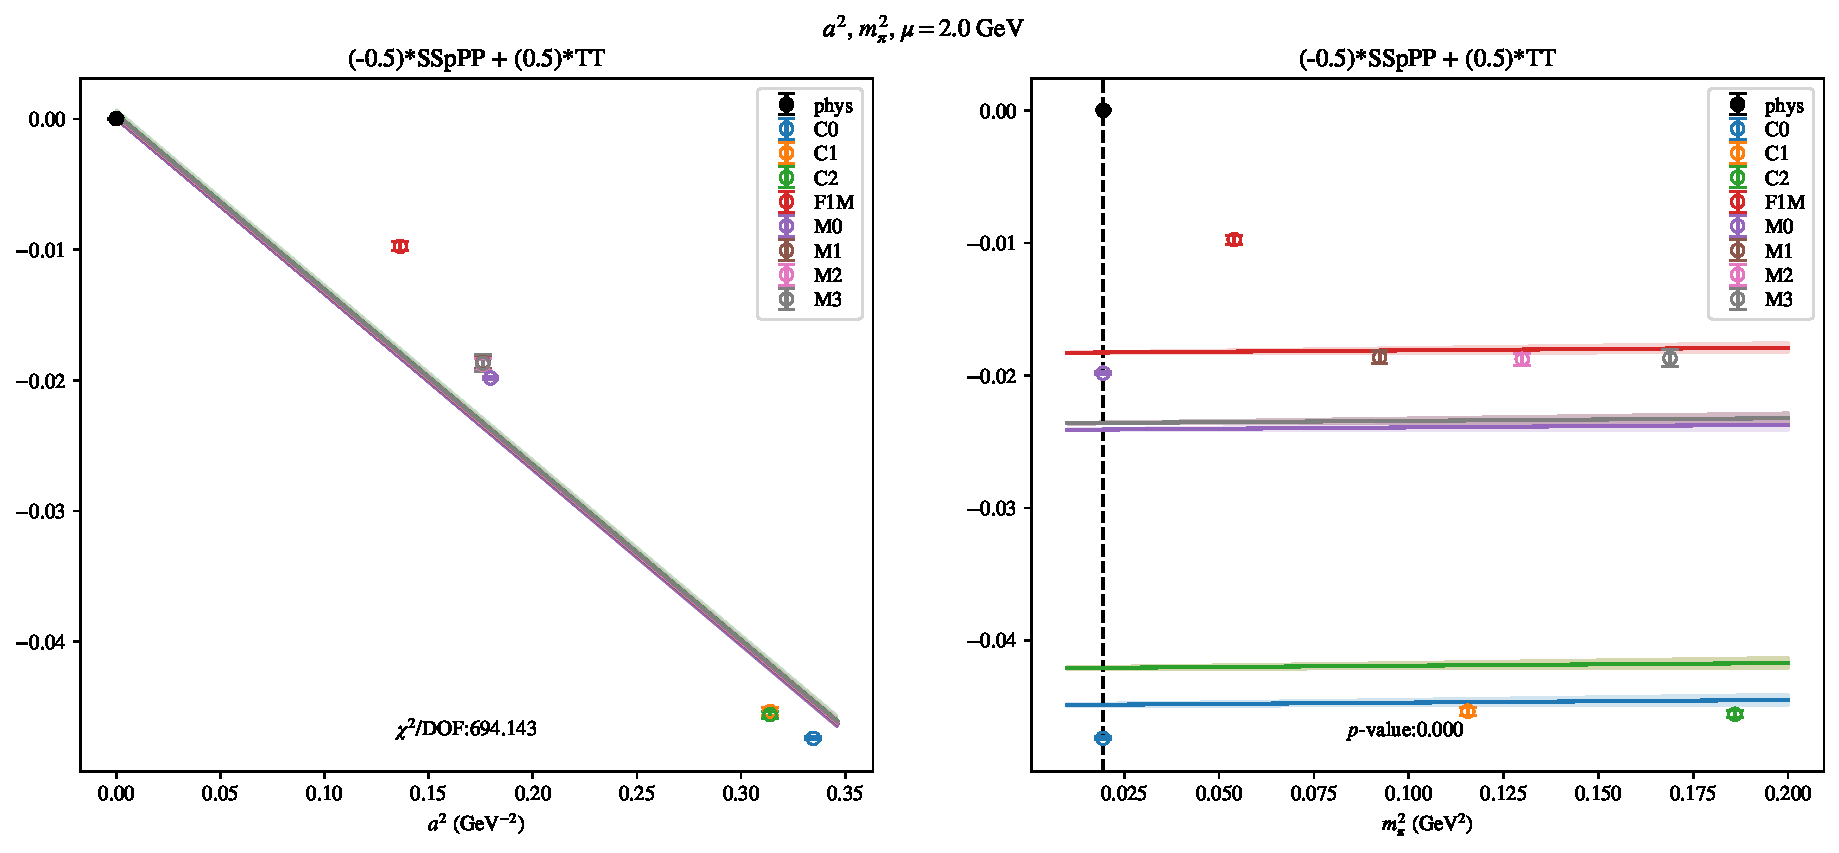
\includepdf[link, pages=-]{SSmPP/a2m2_20.pdf}
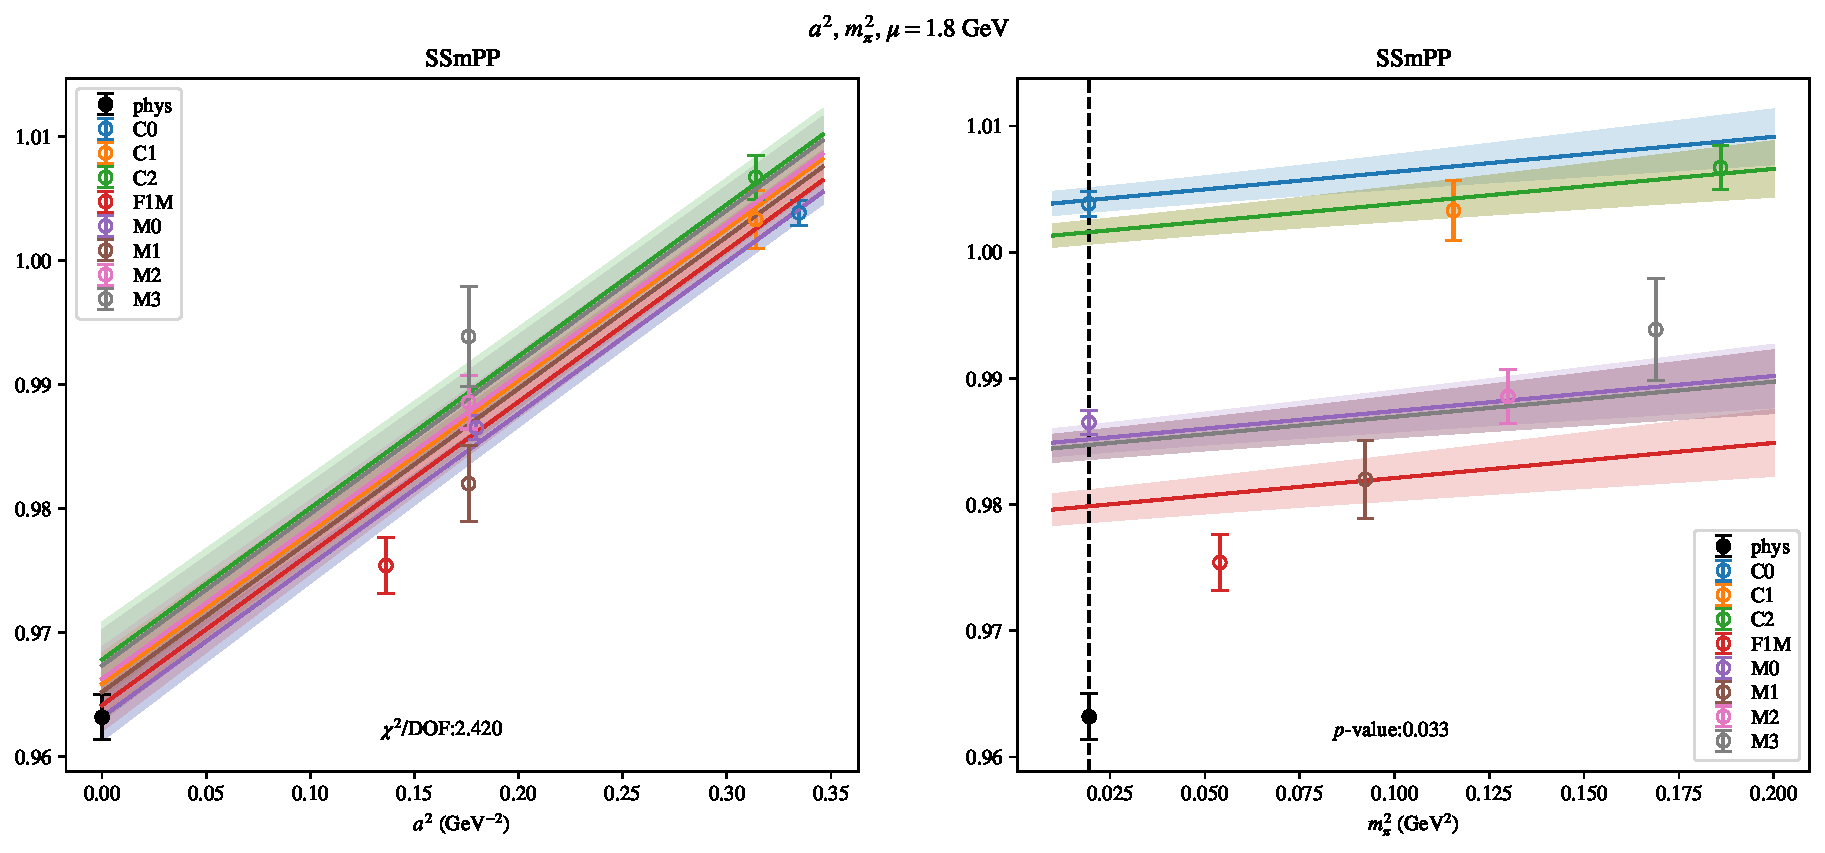
\includepdf[link, pages=-]{SSmPP/a2m2_18.pdf}
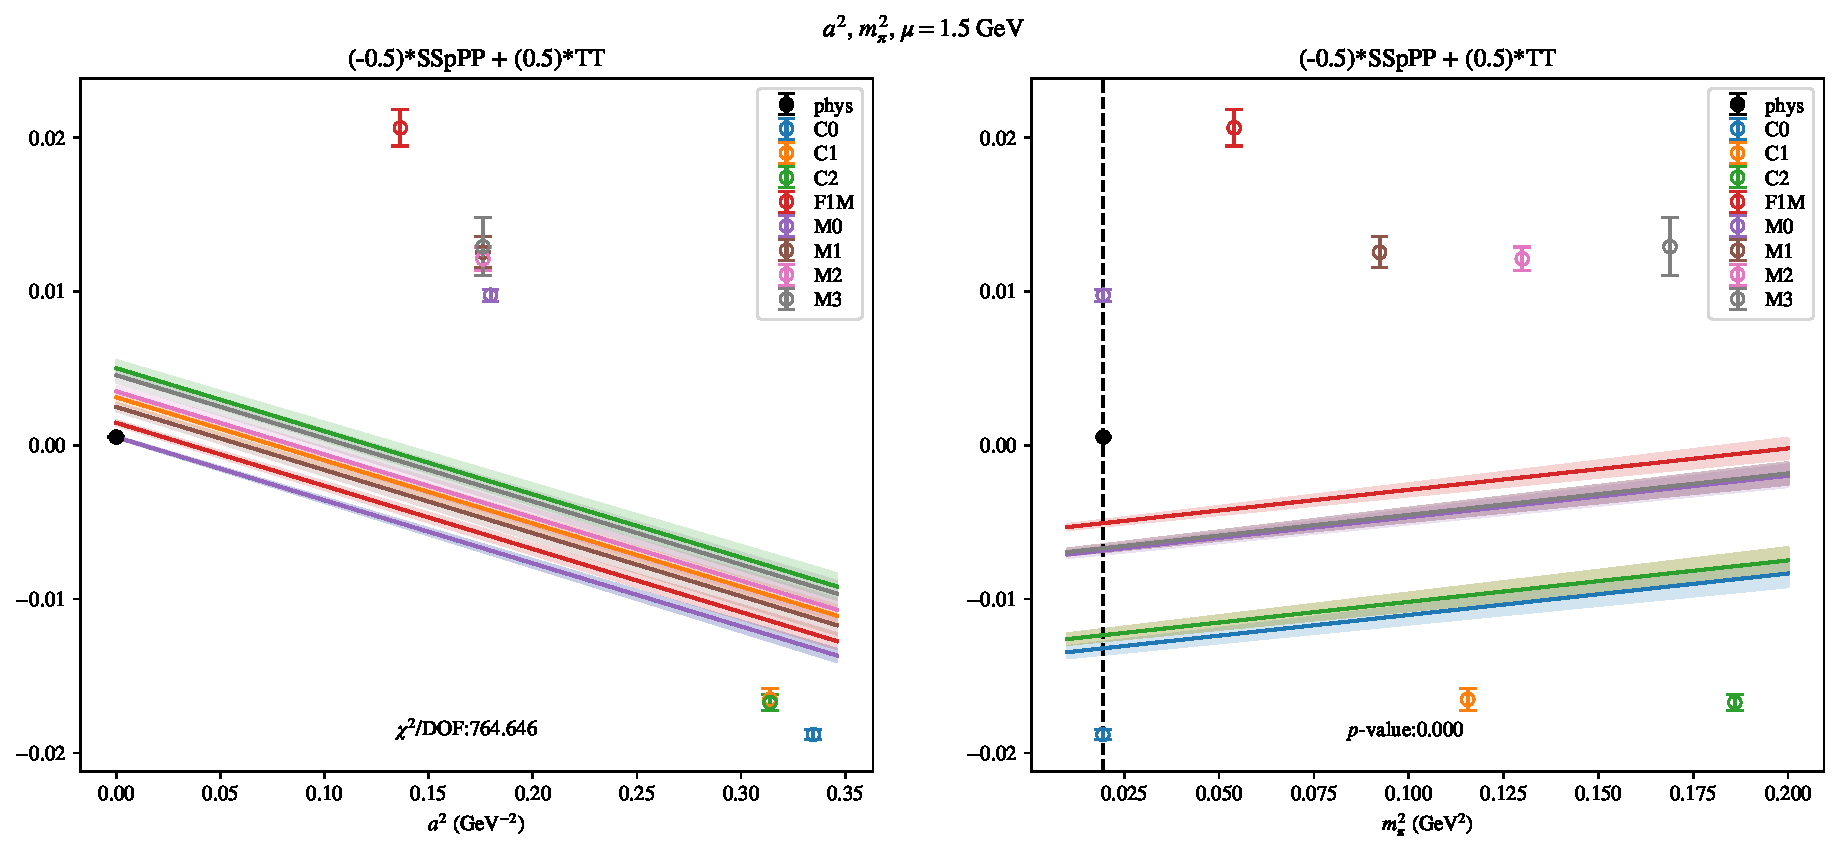
\includepdf[link, pages=-]{SSmPP/a2m2_15.pdf}
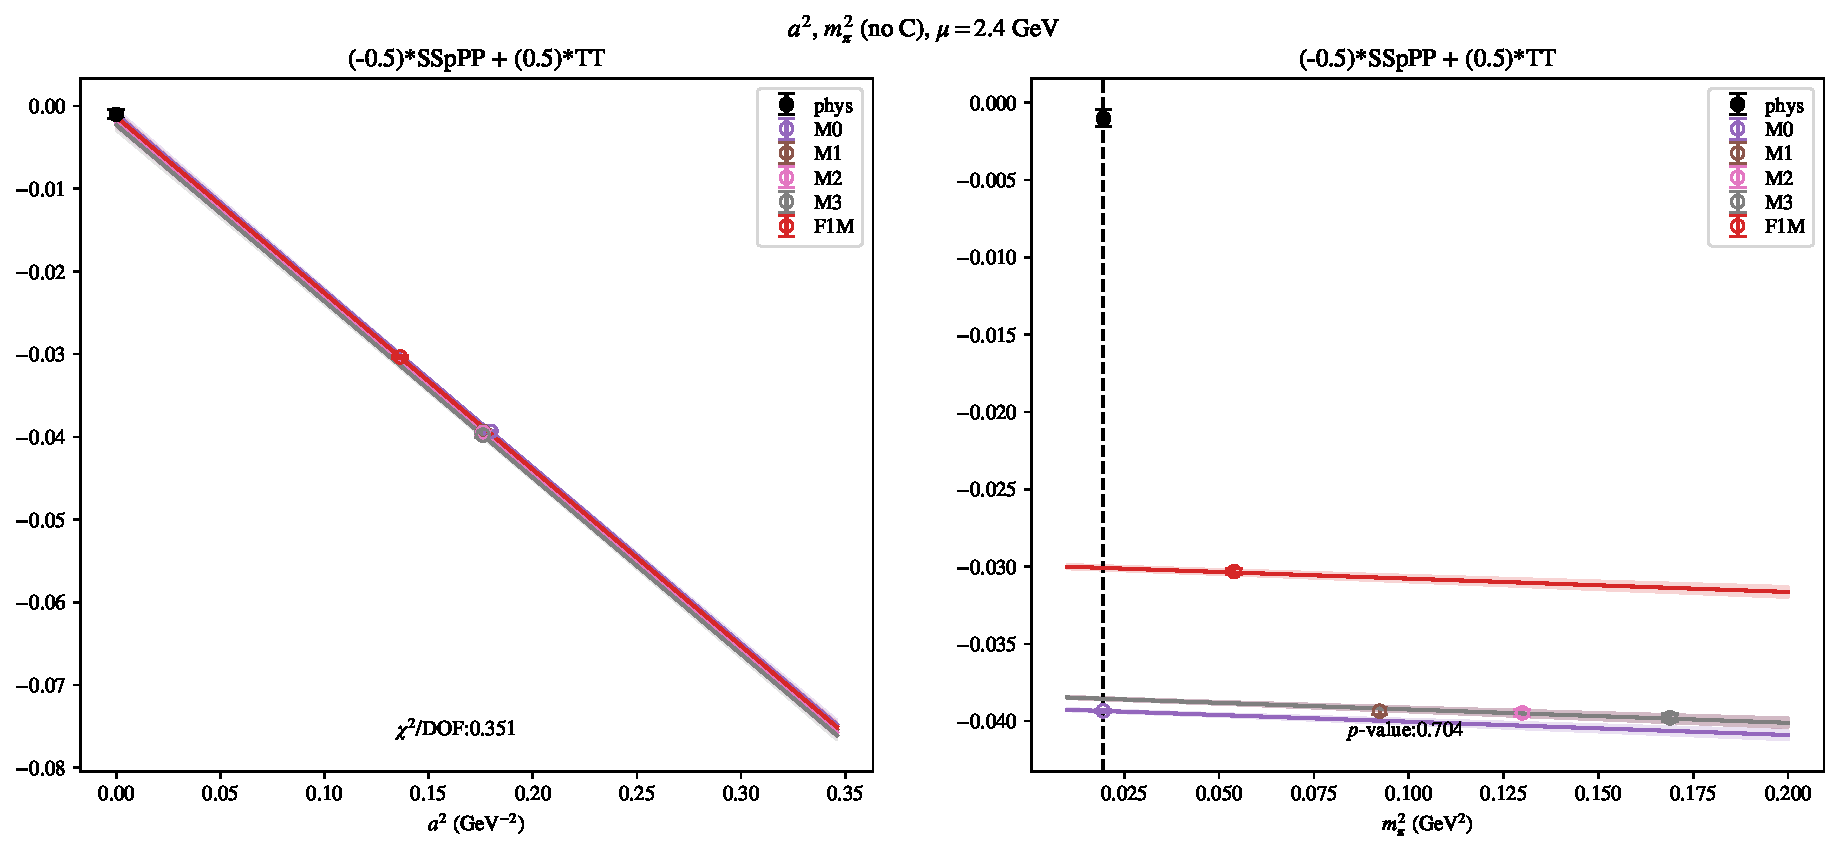
\includepdf[link, pages=-]{SSmPP/a2m2noC_24.pdf}
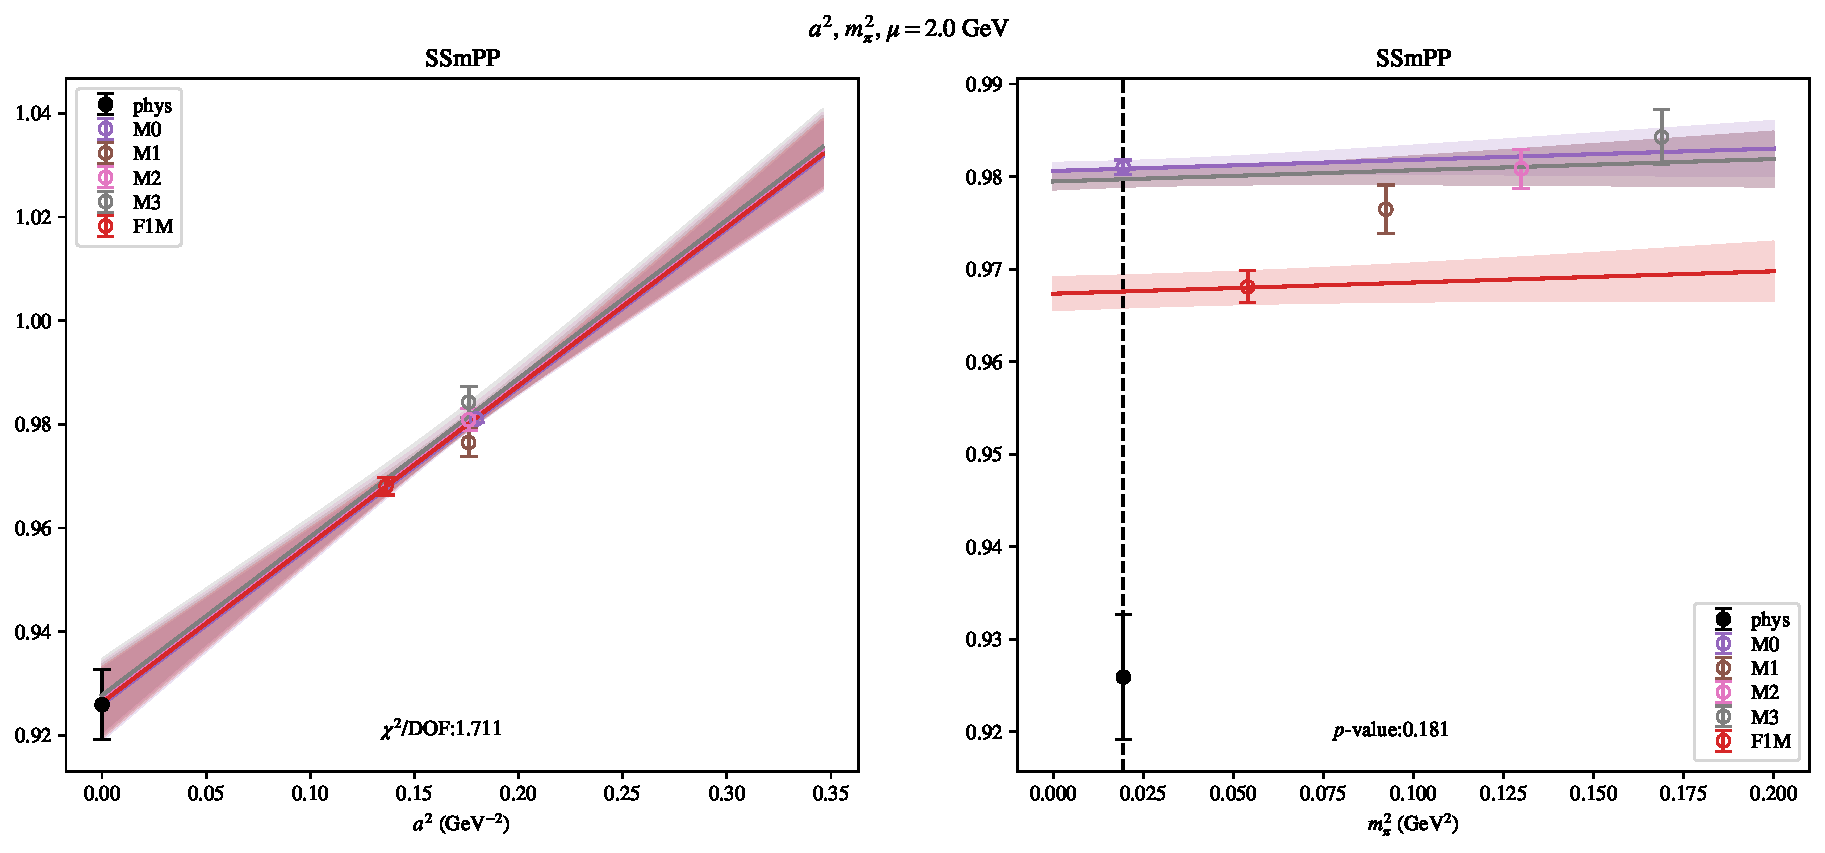
\includepdf[link, pages=-]{SSmPP/a2m2noC_20.pdf}
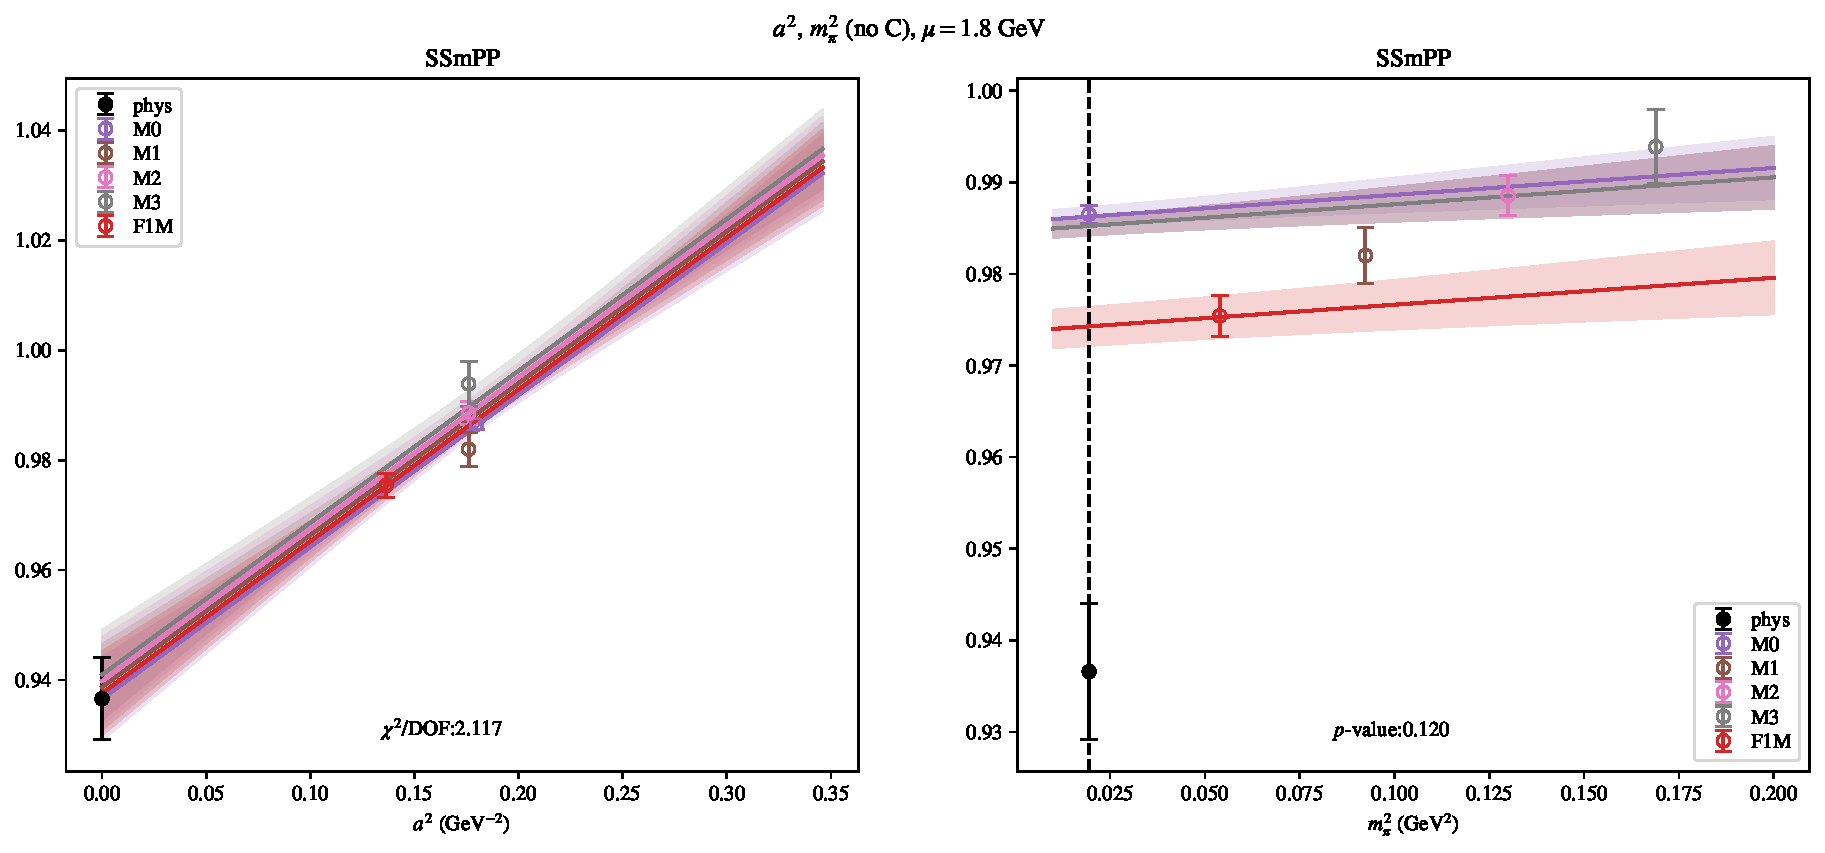
\includepdf[link, pages=-]{SSmPP/a2m2noC_18.pdf}
\includepdf[link, pages=-]{SSmPP/a2m2noC_15.pdf}
\includepdf[link, pages=-]{SSmPP/a2a4m2_24.pdf}
\includepdf[link, pages=-]{SSmPP/a2a4m2_20.pdf}
\includepdf[link, pages=-]{SSmPP/a2a4m2_18.pdf}
\includepdf[link, pages=-]{SSmPP/a2a4m2_15.pdf}
\includepdf[link, pages=-]{SSmPP/a2m2m4_24.pdf}
\includepdf[link, pages=-]{SSmPP/a2m2m4_20.pdf}
\includepdf[link, pages=-]{SSmPP/a2m2m4_18.pdf}
\includepdf[link, pages=-]{SSmPP/a2m2m4_15.pdf}
\includepdf[link, pages=-]{SSmPP/a2m2logm2_24.pdf}
\includepdf[link, pages=-]{SSmPP/a2m2logm2_20.pdf}
\includepdf[link, pages=-]{SSmPP/a2m2logm2_18.pdf}
\includepdf[link, pages=-]{SSmPP/a2m2logm2_15.pdf}
\clearpage
\section{$B_4$}
\begin{table}[h!]
\begin{center}
\begin{tabular}{|c|c|c|c|c|c|}
\hline
$\mu$ (GeV) & $a^2$, $m_\pi^2$& $a^2$, $m_\pi^2$ (no C)& $a^2$, $a^4$, $m_\pi^2$& $a^2$, $m_\pi^2$, $m_\pi^4$& $a^2$, $m_\pi^2$, $\log(m_\pi^2/\Lambda^2)$\\
\hline
2.4& \hyperlink{SSpPP/a2m2_24.pdf.1}{\textbf{0.9436(13)}: 6.273 (0.0)} & \hyperlink{SSpPP/a2m2noC_24.pdf.1}{\textbf{0.9086(66)}: 1.786 (0.168)} & \hyperlink{SSpPP/a2a4m2_24.pdf.1}{\textbf{0.885(10)}: 1.117 (0.346)} & \hyperlink{SSpPP/a2m2m4_24.pdf.1}{\textbf{0.9453(14)}: 5.797 (0.0)} & \hyperlink{SSpPP/a2m2logm2_24.pdf.1}{\textbf{0.9610(14)}: 4.427 (0.0)}\\
2.0& \hyperlink{SSpPP/a2m2_20.pdf.1}{\textbf{0.9557(14)}: 4.069 (0.001)} & \hyperlink{SSpPP/a2m2noC_20.pdf.1}{\textbf{0.9259(67)}: 1.711 (0.181)} & \hyperlink{SSpPP/a2a4m2_20.pdf.1}{\textbf{0.906(11)}: 1.012 (0.4)} & \hyperlink{SSpPP/a2m2m4_20.pdf.1}{\textbf{0.9572(15)}: 3.563 (0.007)} & \hyperlink{SSpPP/a2m2logm2_20.pdf.1}{\textbf{0.9729(15)}: 2.828 (0.015)}\\
1.8& \hyperlink{SSpPP/a2m2_18.pdf.1}{\textbf{0.9631(18)}: 2.42 (0.033)} & \hyperlink{SSpPP/a2m2noC_18.pdf.1}{\textbf{0.9365(74)}: 2.117 (0.12)} & \hyperlink{SSpPP/a2a4m2_18.pdf.1}{\textbf{0.922(12)}: 1.336 (0.254)} & \hyperlink{SSpPP/a2m2m4_18.pdf.1}{\textbf{0.9647(17)}: 1.96 (0.098)} & \hyperlink{SSpPP/a2m2logm2_18.pdf.1}{\textbf{0.9806(18)}: 1.645 (0.144)}\\
1.5& \hyperlink{SSpPP/a2m2_15.pdf.1}{\textbf{0.9741(27)}: 1.372 (0.231)} & \hyperlink{SSpPP/a2m2noC_15.pdf.1}{\textbf{0.9523(94)}: 2.007 (0.134)} & \hyperlink{SSpPP/a2a4m2_15.pdf.1}{\textbf{0.947(15)}: 1.41 (0.228)} & \hyperlink{SSpPP/a2m2m4_15.pdf.1}{\textbf{0.9759(24)}: 1.054 (0.378)} & \hyperlink{SSpPP/a2m2logm2_15.pdf.1}{\textbf{0.9919(28)}: 0.878 (0.495)}\\
\hline
\end{tabular}
\caption{Physical point value from chiral and continuum extrapolation at renormalisation scale $\mu$. Entries are \textbf{value(error)}: $\chi^2/\text{DOF}$ ($p$-value).}
\end{center}
\end{table}
\begin{table}[h!]
\begin{center}
\begin{tabular}{|c c|c|c|c|c|c|}
\hline
$\mu$ (GeV) &  & $a^2$, $m_\pi^2$& $a^2$, $m_\pi^2$ (no C)& $a^2$, $a^4$, $m_\pi^2$& $a^2$, $m_\pi^2$, $m_\pi^4$& $a^2$, $m_\pi^2$, $\log(m_\pi^2/\Lambda^2)$\\
\hline
\multirow{2}{0.5in}{2.4} & $\alpha$ & 0.1681(56)& 0.399(44)& 0.76(11)& 0.1609(60)& 0.1532(55)\\
 & $\beta$ & -0.0001(12)& -0.0001(22)& -0.0003(14)& -0.0020(64)& 0.00464(12)\\
\hline
\multirow{2}{0.5in}{2.0} & $\alpha$ & 0.1378(56)& 0.330(43)& 0.63(11)& 0.1316(60)& 0.1245(55)\\
 & $\beta$ & 0.00023(15)& 0.00022(29)& 0.0& -0.0016(71)& 0.00504(15)\\
\hline
\multirow{2}{0.5in}{1.8} & $\alpha$ & 0.1270(59)& 0.295(46)& 0.52(12)& 0.1206(60)& 0.1135(58)\\
 & $\beta$ & 0.00049(17)& 0.00053(30)& 0.00036(19)& -0.0013(74)& 0.00531(17)\\
\hline
\multirow{2}{0.5in}{1.5} & $\alpha$ & 0.1119(69)& 0.245(53)& 0.36(14)& 0.1047(64)& 0.0981(68)\\
 & $\beta$ & 0.00086(20)& 0.00102(36)& 0.00078(23)& -0.0010(90)& 0.00567(19)\\
\hline
\end{tabular}
\caption{Fit values of coefficients in $B = B_0(1 + \mathbf{\alpha} a^2 + \mathbf{\beta} \frac{m_\pi^2}{f_\pi^2} + \ldots)$.}
\end{center}
\end{table}
\begin{figure}
\centering
\includegraphics[page=1, width=1.1\textwidth]{plots/SSpPP_fit_summary.pdf}
\caption{\\(left) $B_{phys}$ in RI/SMOM scheme from fit variations (fits with $p$-value $<0.05$ marked with ``$\times$"). \\(right) $B_{phys}$ in $\overline{MS}$ computed using $B^{\overline{MS}} = R^{\overline{MS}\leftarrow SMOM}(3.0)\sigma_{npt}^{F1M}(3.0, 2.0) B^{SMOM}$.}
\end{figure}
\clearpage
\includepdf[link, pages=-]{SSpPP/a2m2_24.pdf}
\includepdf[link, pages=-]{SSpPP/a2m2_20.pdf}
\includepdf[link, pages=-]{SSpPP/a2m2_18.pdf}
\includepdf[link, pages=-]{SSpPP/a2m2_15.pdf}
\includepdf[link, pages=-]{SSpPP/a2m2noC_24.pdf}
\includepdf[link, pages=-]{SSpPP/a2m2noC_20.pdf}
\includepdf[link, pages=-]{SSpPP/a2m2noC_18.pdf}
\includepdf[link, pages=-]{SSpPP/a2m2noC_15.pdf}
\includepdf[link, pages=-]{SSpPP/a2a4m2_24.pdf}
\includepdf[link, pages=-]{SSpPP/a2a4m2_20.pdf}
\includepdf[link, pages=-]{SSpPP/a2a4m2_18.pdf}
\includepdf[link, pages=-]{SSpPP/a2a4m2_15.pdf}
\includepdf[link, pages=-]{SSpPP/a2m2m4_24.pdf}
\includepdf[link, pages=-]{SSpPP/a2m2m4_20.pdf}
\includepdf[link, pages=-]{SSpPP/a2m2m4_18.pdf}
\includepdf[link, pages=-]{SSpPP/a2m2m4_15.pdf}
\includepdf[link, pages=-]{SSpPP/a2m2logm2_24.pdf}
\includepdf[link, pages=-]{SSpPP/a2m2logm2_20.pdf}
\includepdf[link, pages=-]{SSpPP/a2m2logm2_18.pdf}
\includepdf[link, pages=-]{SSpPP/a2m2logm2_15.pdf}
\clearpage
\section{$B_5$}
\begin{table}[h!]
\begin{center}
\begin{tabular}{|c|c|c|c|c|c|}
\hline
$\mu$ (GeV) & $a^2$, $m_\pi^2$& $a^2$, $m_\pi^2$ (no C)& $a^2$, $a^4$, $m_\pi^2$& $a^2$, $m_\pi^2$, $m_\pi^4$& $a^2$, $m_\pi^2$, $\log(m_\pi^2/\Lambda^2)$\\
\hline
2.4& \hyperlink{TT/a2m2_24.pdf.1}{\textbf{-0.991(12)}: 8.464 (0.0)} & \hyperlink{TT/a2m2noC_24.pdf.1}{\textbf{-1.035(68)}: 0.597 (0.55)} & \hyperlink{TT/a2a4m2_24.pdf.1}{\textbf{-1.06(10)}: 0.86 (0.487)} & \hyperlink{TT/a2m2m4_24.pdf.1}{\textbf{-0.2526(49)}: 87881.79 (0.0)} & \hyperlink{TT/a2m2logm2_24.pdf.1}{\textbf{-1.009(12)}: 22.717 (0.0)}\\
2.0& \hyperlink{TT/a2m2_20.pdf.1}{\textbf{-1.185(15)}: 8.812 (0.0)} & \hyperlink{TT/a2m2noC_20.pdf.1}{\textbf{-1.235(81)}: 0.354 (0.702)} & \hyperlink{TT/a2a4m2_20.pdf.1}{\textbf{-1.27(13)}: 0.418 (0.796)} & \hyperlink{TT/a2m2m4_20.pdf.1}{\textbf{-0.3121(69)}: 78664.389 (0.0)} & \hyperlink{TT/a2m2logm2_20.pdf.1}{\textbf{-1.206(16)}: 22.093 (0.0)}\\
1.8& \hyperlink{TT/a2m2_18.pdf.1}{\textbf{-1.298(21)}: 8.923 (0.0)} & \hyperlink{TT/a2m2noC_18.pdf.1}{\textbf{-1.346(97)}: 0.993 (0.371)} & \hyperlink{TT/a2a4m2_18.pdf.1}{\textbf{-1.41(15)}: 2.489 (0.041)} & \hyperlink{TT/a2m2m4_18.pdf.1}{\textbf{-0.3267(89)}: 55018.954 (0.0)} & \hyperlink{TT/a2m2logm2_18.pdf.1}{\textbf{-1.321(21)}: 17.569 (0.0)}\\
1.5& \hyperlink{TT/a2m2_15.pdf.1}{\textbf{-1.468(32)}: 9.386 (0.0)} & \hyperlink{TT/a2m2noC_15.pdf.1}{\textbf{-1.51(13)}: 1.469 (0.23)} & \hyperlink{TT/a2a4m2_15.pdf.1}{\textbf{-1.61(21)}: 5.497 (0.0)} & \hyperlink{TT/a2m2m4_15.pdf.1}{\textbf{-0.342(12)}: 31220.791 (0.0)} & \hyperlink{TT/a2m2logm2_15.pdf.1}{\textbf{-1.495(33)}: 13.802 (0.0)}\\
\hline
\end{tabular}
\caption{Physical point value from chiral and continuum extrapolation at renormalisation scale $\mu$. Entries are \textbf{value(error)}: $\chi^2/\text{DOF}$ ($p$-value).}
\end{center}
\end{table}
\begin{table}[h!]
\begin{center}
\begin{tabular}{|c c|c|c|c|c|c|}
\hline
$\mu$ (GeV) &  & $a^2$, $m_\pi^2$& $a^2$, $m_\pi^2$ (no C)& $a^2$, $a^4$, $m_\pi^2$& $a^2$, $m_\pi^2$, $m_\pi^4$& $a^2$, $m_\pi^2$, $\log(m_\pi^2/\Lambda^2)$\\
\hline
\multirow{2}{0.5in}{2.4} & $\alpha$ & -0.578(37)& -0.79(32)& -1.12(78)& -(54)& -0.582(37)\\
 & $\beta$ & 0.00087(10)& 0.00090(18)& 0.001053(99)& -6(61)& 0.00561(10)\\
\hline
\multirow{2}{0.5in}{2.0} & $\alpha$ & -0.681(36)& -0.88(31)& -1.27(76)& -(15)& -0.682(35)\\
 & $\beta$ & 0.00112(12)& 0.00147(23)& 0.00129(12)& -7(27)& 0.00590(12)\\
\hline
\multirow{2}{0.5in}{1.8} & $\alpha$ & -0.703(37)& -0.89(33)& -1.35(80)& (14)& -0.705(37)\\
 & $\beta$ & 0.00087(13)& 0.00166(24)& 0.00109(13)& -(17)& 0.00566(13)\\
\hline
\multirow{2}{0.5in}{1.5} & $\alpha$ & -0.733(40)& -0.89(38)& -1.47(91)& (11)& -0.735(39)\\
 & $\beta$ & 0.00056(14)& 0.00188(26)& 0.00086(14)& -(13)& 0.00535(13)\\
\hline
\end{tabular}
\caption{Fit values of coefficients in $B = B_0(1 + \mathbf{\alpha} a^2 + \mathbf{\beta} \frac{m_\pi^2}{f_\pi^2} + \ldots)$.}
\end{center}
\end{table}
\begin{figure}
\centering
\includegraphics[page=1, width=1.1\textwidth]{plots/TT_fit_summary.pdf}
\caption{\\(left) $B_{phys}$ in RI/SMOM scheme from fit variations (fits with $p$-value $<0.05$ marked with ``$\times$"). \\(right) $B_{phys}$ in $\overline{MS}$ computed using $B^{\overline{MS}} = R^{\overline{MS}\leftarrow SMOM}(3.0)\sigma_{npt}^{F1M}(3.0, 2.0) B^{SMOM}$.}
\end{figure}
\clearpage
\includepdf[link, pages=-]{TT/a2m2_24.pdf}
\includepdf[link, pages=-]{TT/a2m2_20.pdf}
\includepdf[link, pages=-]{TT/a2m2_18.pdf}
\includepdf[link, pages=-]{TT/a2m2_15.pdf}
\includepdf[link, pages=-]{TT/a2m2noC_24.pdf}
\includepdf[link, pages=-]{TT/a2m2noC_20.pdf}
\includepdf[link, pages=-]{TT/a2m2noC_18.pdf}
\includepdf[link, pages=-]{TT/a2m2noC_15.pdf}
\includepdf[link, pages=-]{TT/a2a4m2_24.pdf}
\includepdf[link, pages=-]{TT/a2a4m2_20.pdf}
\includepdf[link, pages=-]{TT/a2a4m2_18.pdf}
\includepdf[link, pages=-]{TT/a2a4m2_15.pdf}
\includepdf[link, pages=-]{TT/a2m2m4_24.pdf}
\includepdf[link, pages=-]{TT/a2m2m4_20.pdf}
\includepdf[link, pages=-]{TT/a2m2m4_18.pdf}
\includepdf[link, pages=-]{TT/a2m2m4_15.pdf}
\includepdf[link, pages=-]{TT/a2m2logm2_24.pdf}
\includepdf[link, pages=-]{TT/a2m2logm2_20.pdf}
\includepdf[link, pages=-]{TT/a2m2logm2_18.pdf}
\includepdf[link, pages=-]{TT/a2m2logm2_15.pdf}
\end{document}